\documentclass{ZJUthesis}
\hypersetup{colorlinks=true}
\begin{document}
%%%%%%%%%%%%%%%%%%%%%%%%%%%%%
%% 正文字体设定
%%%%%%%%%%%%%%%%%%%%%%%%%%%%%
\fangsong

%%%%%%%%%%%%%%%%%%%%%%%%%%%%%
%% 论文封面部分
%%%%%%%%%%%%%%%%%%%%%%%%%%%%%
\classification{TN292.11}
\serialnumber{10335}
\SecretLevel{无}
\PersonalID{10930020}

\title{基于量子阱混杂技术的快速波长}
\titletl{可切换V型耦合腔半导体激光器研究}

\Etitle{Fast Wavelength Switchable V-Coupled}
\Etitletl{Cavity Semiconductor Laser based on}
\Etitletll{Quantum Well Intermixing Technology}

\author{张欣}
\degree{博士}

\supervisor{何建军}
\major{光学工程}
\researchdm{集成光电子}
\institute{光电科学与工程学院}

\submitdate{2015年10月20日}

\makeCoverPage

%%%%%%%%%%%%%%%%%%%%%%%%%%%%%%
%% 中文题名页内容
%%%%%%%%%%%%%%%%%%%%%%%%%%%%%%
\reviewersA{匿名1}
\reviewersB{匿名2}
\reviewersC{匿名3}
\reviewersD{匿名4}
\reviewersE{匿名5}

\chairman{陆璇辉\hspace{1.5em}教授\hspace{1.5em}浙江大学}
\commissionerA{庄飞\hspace{1.5em}教授\hspace{1.5em}杭州师范大学}
\commissionerB{乐孜纯\hspace{1.5em}教授\hspace{1.5em}浙江工业大学}
\commissionerC{章坚武\hspace{1.5em}教授\hspace{1.5em}杭州电子科技大学}
\commissionerD{董新永\hspace{1.5em}教授\hspace{1.5em}中国计量大学}

\defenddate{2015年12月14日}

\maketitle
%%%%%%%%%%%%%%%%%%%%%%%%%%%%%%
%% 英文封面内容,硕士论文可不要此页
%%%%%%%%%%%%%%%%%%%%%%%%%%%%%%
% \englishtitle{Fast Wavelength Switchable V-Coupled Cavity Semiconductor}
% \englishtitletl{Laser based on Quantum Well Intermixing Technology}

\EreviewersA{Anonymous One}
\EreviewersB{Anonymous Two}
\EreviewersC{Anonymous Three}
\EreviewersD{Anonymous Four}
\EreviewersE{Anonymous Five}

\Echairman{Xuanhui Lu\hspace{1em}Prof.\hspace{1em}Zhejiang Univ.}
\EcommissionerA{Fei Zhuang\hspace{1em}Prof.\hspace{1em}Hangzhou Normal Univ.}
\EcommissionerB{Zichun Le\hspace{1em}Prof.\hspace{1em}Zhejiang Univ. of Tech.}
\EcommissionerC{Jianwu Zhuang\hspace{1em}Prof.\hspace{1em}Hangzhou Dianzi Univ.}
\EcommissionerD{Xinyong Dong\hspace{1em}Prof.\hspace{1em}China Jiliang Univ.}

\Edefenddate{December 14, 2015}

\makeenglishtitle
%%%%%%%%%%%%%%%%%%%%%%%%%%%%%%
%% 原创声明与版权协议页
%%%%%%%%%%%%%%%%%%%%%%%%%%%%%%
\makeOSandCPRTpage

%%%%%%%%%%%%%%%%%%%%%%%%%%%%%%
%% 论文部分开始
%%%%%%%%%%%%%%%%%%%%%%%%%%%%%%
\ZJUfrontmatter

%%%%%%%%%%%%%%%%%%%%%%%%%%%%%%
%% 致谢页
%%%%%%%%%%%%%%%%%%%%%%%%%%%%%%
\begin{thanks}

在即将完成学业的时候,想起自己在求是园度过的十年半的时光,我百感交集。人的一生说来很短暂,而青春的岁月更是屈指可数。我将生命中最美好的时光献给这里,我无怨无悔。同时,我也心存感激,感谢身边所有的人,陪我度过这人生中最美好的时光。

首先,我要感谢我的父母。看着身边的孩子早早的工作、成家,甚至有了自己的孩子,我想你们的等待似乎太漫长了一些。爸爸妈妈,你们为我骄傲,我为你们骄傲。

然后,我要感谢我的导师何建军教授。何老师渊博的学识、严谨的态度让我终生难忘,他精益求精、一丝不苟的工作作风让我敬佩不已。非常感谢何老师科研上的精心栽培和生活上的热心关怀。

接着,我要感谢加拿大Sherbrooke大学的Jan~J.~Dubowski教授和刘能师姐。在我的量子阱混杂实验陷入苦战的时候,他们的指导给了我很大的帮助。没有他们的帮助,我很难完成后面的实验。

同时,我要感谢实验室所有成员对我工作的大力支持和帮助。感谢彭盛华师兄带领我进入课题,给予我学术上的启蒙性的指导和建议。感谢Kaleem陪伴我做了两年的量子阱混杂实验。感谢李明宇博士、王磊博士、刘德坤、金嘉亮、金磊、马骁、朱洪力、邹立等师兄对我的关怀和照顾。感谢庄园、孟剑俊、邓浩瑜等同学在学术上的大力支持。感谢紫金港东五的时尧成博士、胡师傅、陈辉对我实验的大力帮助。感谢光电系设备管理员陈莉英老师、孙玉霞老师对KrF准分子激光器使用的大力支持。这一切都会成为我一生美好而难忘的回忆。

最后,我要感谢为我辛苦服务了六年半的超净室和教三的实验设备,特别是牛津ICP、快速退火炉、有源和无源测试台、PL测试系统和KrF准分子激光器。在我的眼里,你们一直是有生命的存在。

\end{thanks}
%%%%%%%%%%%%%%%%%%%%%%%%%%%%%%
%% 摘要
%%%%%%%%%%%%%%%%%%%%%%%%%%%%%%
\begin{abstract}

电信业进入二十一世纪之后,对网络带宽的需求还在持续增加。波分复用技术(WDM)、大范围可调谐激光器和单片集成技术的出现,极大地增加了每个光纤内传送的数据量,同时降低了光通信器件的制作成本。在过去的几十年中,量子阱混杂技术(QWI)被证明为一种简单有效的实现单片集成的方法。而其中的KrF准分子激光器量子阱混杂技术由于效果好、稳定性好,逐渐成为了最有希望的方法之一。

在本文中,利用实验室现有的KrF准分子激光器开发了基于紫外激光照射的量子阱混杂技术。首次应用这项技术成功制作了FP激光器和无源波导。测试得到的FP激光器和无源波导的性能甚至比量子阱混杂之前的性能更好。随后,我们将该技术应用到V型腔激光器中,首次实现了基于载流子注入的波长调谐功能。其中腔长差5\%的器件可以实现1550~nm波段100~GHz间隔的32个通道的单电极调谐,同时边模抑制比(SMSR)可以达到35~dB,与热调谐的V型腔激光器可以媲美。此外,调谐电流仅0$\sim$40~mA,比热调谐的电流(>100~mA)小得多。最后,我们分析了该激光器的波长切换性能。相邻通道的切换时间仅1~ns左右,比热调谐的时间快了4个数量级。我们还研究了间隔通道数对切换时间的影响,发现随着间隔通道数增加,波长切换时间也随之增加,最后在10~ns左右趋于饱和。这种单电极控制的快速波长可切换半导体激光器在未来的波长路由光网络中有广阔的应用前景。

\keywords{集成光路,量子阱,量子阱混杂,可调谐激光器}
\end{abstract}
%%%%%%%%%%%%%%%%%%%%%%%%%%%%%%
%% 英文摘要
%%%%%%%%%%%%%%%%%%%%%%%%%%%%%%
\begin{englishabstract}

As the telecommunications industry enters the twenty-first century, the demand for network bandwidth continues to increase. The emergence of wavelength division multiplexing (WDM), widely tunable semiconductor lasers and monolithic integration technique have greatly increased the amount of data transmitted within each fiber, while reducing the manufacturing cost of optical components. In the past few decades, quantum well intermixing (QWI) technique was proved to be a simple and effective way to achieve monolithic integration. The KrF excimer laser based QWI technology has been demonstrated to be one of the most promising methods because of the large bandgap shift and good stability.

In this thesis, we developed the UV laser based QWI technology with the KrF excimer laser in the lab and successfully produced FP lasers and passive waveguides using this technology. The tested performances of FP lasers and passive waveguides are even better than the performances before quantum well intermixing. Then, we apply this technique to the V-coupled cavity laser, realizing the carrier injection-based wavelength tuning effect for the first time. The laser wavelength can be switched between 32~channels at 100~GHz spacing using a single electrode control, while side-mode suppression ratio (SMSR) reaches 35~dB, comparable with heat-tuning V-cavity lasers. In addition, the tuning current is 0 $\sim$ 40~mA, much smaller than the current (> 100~mA) of heat-tuning laser. Finally, we analyzed the performance of the laser wavelength switching. Switching time for adjacent channels is only about 1~ns, four orders of magnitude faster than the time of heat tuning. We also studied the influence of the intermediate numbers of channels for the switching time, and found that as the intermediate numbers of channels increase, the wavelength switching time also increases, and finally saturate at around 10~ns. The single-electrode controlled fast wavelength switching is very promising for future wavelength routed optical networks.

\englishkeywords{photonic integrated circuit, quantum well, quantum well intermixing, tunable semiconductor laser}
\end{englishabstract}
%%%%%%%%%%%%%%%%%%%%%%%%%%%%%%
%% 目录页
%%%%%%%%%%%%%%%%%%%%%%%%%%%%%%
\ZJUcontents
%%%%%%%%%%%%%%%%%%%%%%%%%%%%%%
%% 正文内容部分开始
%%%%%%%%%%%%%%%%%%%%%%%%%%%%%%
\ZJUmainmatter



%%%%%%%%%%%%%%%%%%%%
\chapter{绪论}
%%%%%%%%%%%%%%%%%%%%

随着时代的进步,光通信技术作为引领人类信息革命的关键技术,正在蓬勃和飞速的发展。而光通信的芯片制造技术,又是光通信技术中门槛最高,附加值最大的技术,也是整个光通信领域最核心的技术。可以说,谁掌握了芯片制造的前沿技术,谁就站在了光通信技术的制高点上。近年来,集成光路技术正在逐渐被人们所重视,并成为了芯片制造的前沿技术。在接下来的内容中,集成光路技术将被详细讨论。

%%%%%%%%%%%%%%%%%%%%
\section{光通信技术的未来发展趋势}
%%%%%%%%%%%%%%%%%%%%

1966年,英籍华裔学着高锟博士开创性地提出了利用光纤进行通信的基本原理,并预言了制造用于通信的超低损耗的光纤的可能性\cite{kao1966dielectric}。从那以后,全世界掀起了一场光纤通信的革命,人类进入了光通信的时代。如今,人们的对光通信网络的带宽需求仍然在不断上升。图~\ref{fig_akamai}~是Akamai公司统计的2009年以来全世界和中国大陆的平均网速的变化趋势。从图中可以看出,这两个地区的平均网速在最近的六年内依然保持指数型增长,说明光通信产业还有很大的发展潜力。类似于集成电路领域的摩尔定律,光通信领域也遵循同样的规律。另外,中国作为世界第二大经济体,平均网速还不到全世界的平均水平,这也说明了中国光通信产业还有很大的发展空间。另一方面,光通信器件的价格也在指数型下降。对于市场上比较成熟的光通信器件来说,各个公司竞争的根本就是价格的竞争。除了研究最前沿的技术之外,研究用更简单的方法、更低的成本制作出性能可以相媲美的器件,也是一个突破口。

\begin{figure}[htbp]
  \centering
  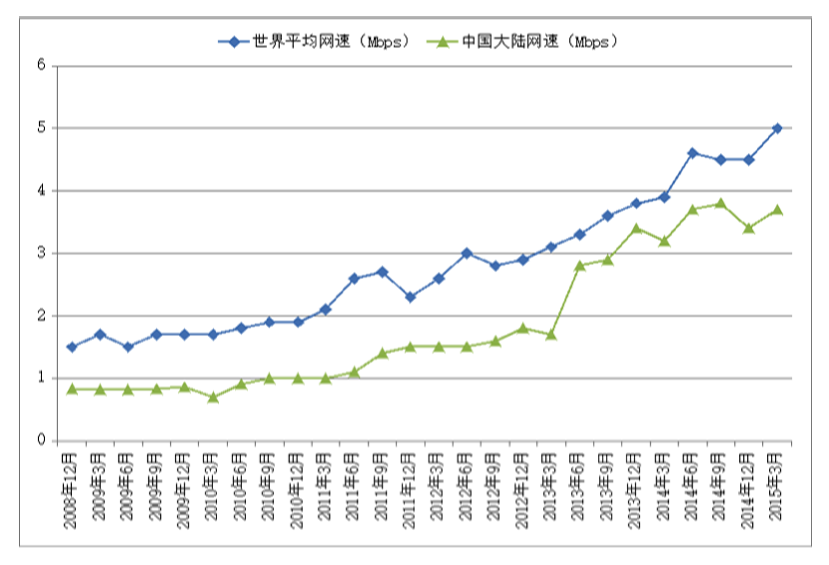
\includegraphics[width=0.7\textwidth]{./Pictures/akamai.eps}\\
  \caption{Akamai公司统计的六年来全世界和中国大陆的平均网速}
  \label{fig_akamai}
\end{figure}

一个最基本的光通信系统如图~\ref{fig_system}所示。这个系统通常包含光发射机、光纤和光接收机三个部分。其中的发射机是由电路驱动的半导体激光器组成,其中的信号由高频电信号直接加到激光器或调制器上,变成光信号。光信号由光纤经过一定距离的传输到达接收机,由接收机的光探测器转换为电信号。如今的光纤,例如1550~nm单模光纤的损耗可以做到0.2~dB/km以内,再加上掺铒光纤放大器(EDFA)\cite{Tachibana1991Erbium}\cite{Laming1992Erbium}、拉曼放大器\cite{Bromage2004Raman}等技术的发明,光通信技术在光的传输上已经比较成熟。理论上光纤传输光的带宽极限是100~Tb/s,所以限制光通信系统带宽的瓶颈往往在于光发射机上。对于由单个固定波长的激光器构成的光发射机来说,调制方式决定了带宽。最早的直接调制的速度最快在1~GHz量级\cite{Utaka1981Single}\cite{Saito2001Low},这已经不能满足需要。电吸收调制的速度在10~GHz量级\cite{Ido1996Ultra},目前的商业系统主要就是采用了这种方法,可以达到40~GHz的标准。行波电极调制还处在实验室研究阶段,速度在50~GHz$\sim$100~GHz量级\cite{Kawano1997Polarisation}\cite{Li1999Ultrahigh}\cite{Irmscher2002InP}~,距离商业应用还有一段距离。如果要再往上提高速度,就可能遇到很大的难度。

\begin{figure}[htbp]
  \centering
  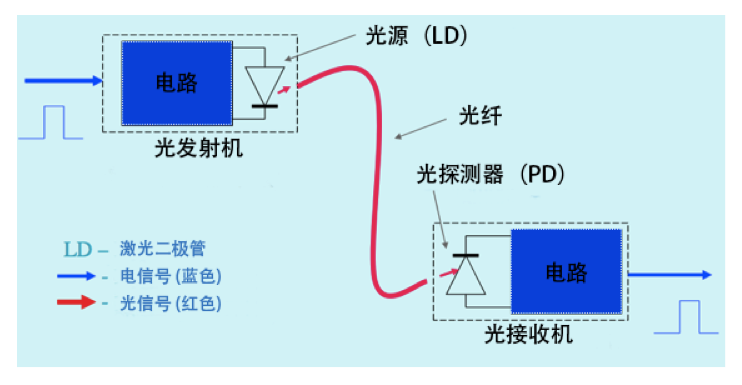
\includegraphics[width=0.7\textwidth]{./Pictures/system.eps}\\
  \caption{光通信系统示意图}
  \label{fig_system}
\end{figure}

为了更好的利用光纤传输的波长窗口和100~T的带宽上限,人们采用了波分复用(WDM)的技术。由于不同波长的光在光纤中传输是基本不会互相干扰的,所以可以将许多不同波长的光同时由发射机发射到光纤内,每一种波长携带不同的信号,这样就大大增加了光纤的利用率,也就是增加了整个光通信系统的带宽。图~\ref{fig_wdm}~展示了波分复用技术的光谱。人们把光纤的1310~nm和1550~nm波段连接起来,划分成六个连续的波段,用来传输不同波长的光信号。其中光纤损耗最低的1530~nm$\sim$1610~nm范围被定义为密集波分复用(DWDM)波段,他包含了整个C波段和L波段。每个通道的波长间隔是由国际电信联盟(ITU)决定的,频率间隔在通常在12.5~GHz(0.1nm)到100~GHz(0.8nm)范围内。由于每个信道的频率间隔比较小,所以被称为密集波分复用。密集的频率间隔意味着更高的带宽和更高的成本,所以适用于长距离传输的光通信系统。此外,人们还将1271~nm到1611~nm、间隔20~nm的这些信道定义为稀疏波分复用(CWDM)信道。由于稀疏波分复用的频率间隔很大,意味着更低的带宽和更低的成本,所以适用于城际网等短距离的光通信系统。密集波分复用和稀疏波分复用作为不同的WDM标准,会同时出现在未来的光通信系统中。

\begin{figure}[htbp]
  \centering
  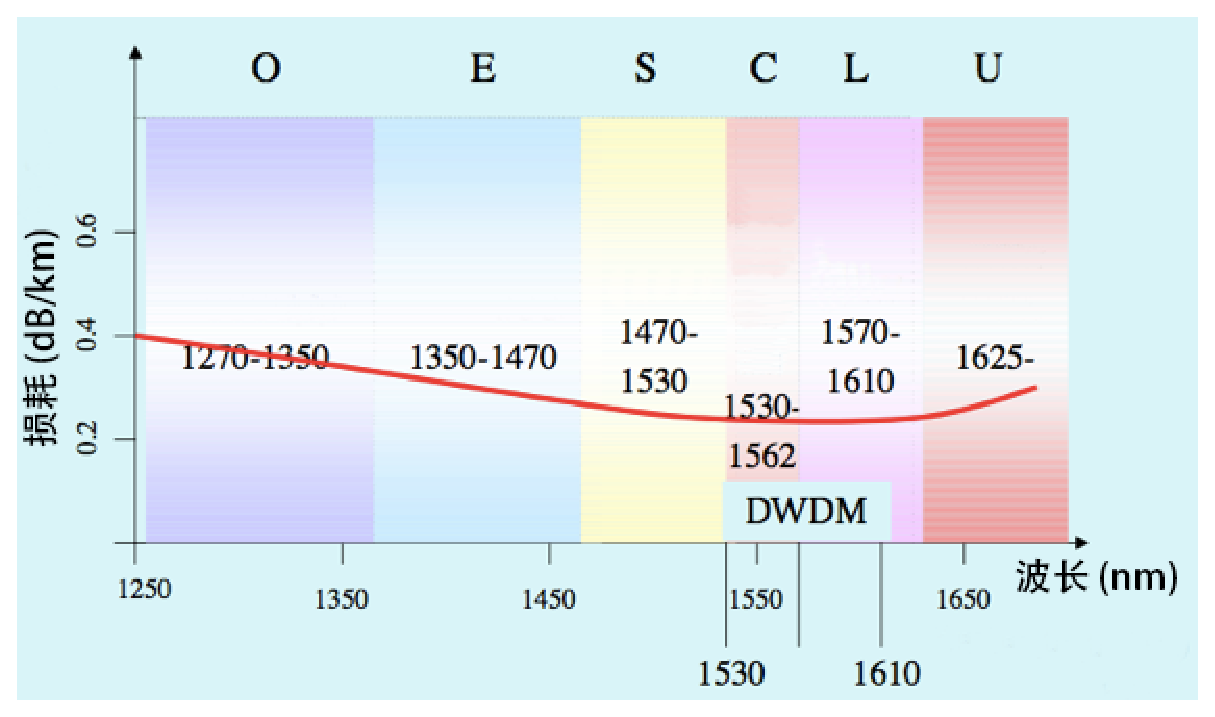
\includegraphics[width=0.7\textwidth]{./Pictures/wdm.eps}\\
  \caption{波分复用技术光谱}
  \label{fig_wdm}
\end{figure}

这里举个例子,对于密集波分复用间隔100~GHz的情况,总共有80~nm/0.8~nm=100个通道可以利用。假设每个通道传输速率是40~GHz,那么总的带宽是100×40~GHz=4~THz。一方面,采用密集波分复用技术大大增加了光通信系统的带宽,另一方面,距离光纤100~THz的极限仍然有很大的距离。即便如此,想要实现密集波分复用的方案也并非易事。想象一下,要制作200个波长完全不同的激光器、200个与激光器对应的调制器、200通道的阵列波导光栅(AWG)或刻蚀衍射光栅(EDG),并且用光纤或波导连接起来,将会是一个非常复杂和昂贵的光发射机。

为了适应波分复用技术对光发射机的复杂度要求,人们提出了集成光路的概念。集成光路的想法源于集成电路。在集成电路中,成千上万的电阻、电容、电感、晶体管等等器件可以被集成到一块芯片中。例如,Intel公司可以在一块Si晶片上集成20亿个晶体管。与分立器件相比,集成电路有很多优势,比如说重量小,体积小,发热小,价格低。参考集成电路的现状,人们提出了集成光路的概念,也就是将成千上万个光器件,例如激光器、调制器、放大器、波导、阵列波导光栅等等器件集成到一块芯片上,这样同样会拥有重量小,体积小,发热小,价格低等等优点。更重要的是,在光器件领域,芯片的封装占整个器件的成本的比重非常高,有时候甚至超过90\%。当所有的器件集成到一块芯片上之后,原来的多次封装变成了一次封装,这样就可以大大减少成本。另一个问题是分立器件之间存在很大的耦合损耗。在器件之间使用模式转换器等组件,是半导体芯片减少耦合损耗的有效方法,但它仍然是光损耗的一个主要来源。而所有器件集成在一块芯片上之后,这个问题就迎刃而解了。自从集成光路的想法被提出以来,人们已经可以在实验室制作一些不太复杂的集成器件,而在实际的商业应用中还不多,或者集成的程度还很低。光通信器件未来的发展中,集成化将会是一条必由之路。

以上介绍了光通信领域的一些比较接近商用的技术。实际上,人们将现代光电子学运用到光通信领域时,开辟了很多全新的研究方向,例如等离子体激元学、纳米光子学、硅光子学、光子晶体、超材料、慢光和快光、单光子操纵等等。比如说,等离子体激元学就是其中一个比较热门的方向。他的原理就是光在介质和金属的界面传播时,会引发金属内的电子与光的互相作用,形成电子和光波的混合波。这种混合波可以超越光的衍射极限,将光传输的尺寸进一步缩小。利用相关的性质,人们已经在实验室制作出新型的激光器\cite{Jones2009Photonic}、LED、THz调制器\cite{Fattal2008Design}、探测器\cite{Palmer2009Surface}等等,这让人们看到了光通信技术的未来发展方向。
%%%%%%%%%%%%%%%%%%%%
\section{集成光路技术}
%%%%%%%%%%%%%%%%%%%%

集成光路技术发展到今天,出现了混合集成和单片集成两种方式。他们与分立器件的关系如图~\ref{fig_integrations}~所示。单片集成是将所有器件集成在同一块芯片中,而混合集成是集成在两块或几块芯片中,然后再将他们用某种方式固定起来。所以,从分立器件到混合集成,再到单片集成,整个芯片所包含的器件逐渐增加,成熟度逐渐提高,同时复杂度逐渐下降,成本也随之下降。下面我们详细讨论这两种技术。

\begin{figure}[htbp]
  \centering
  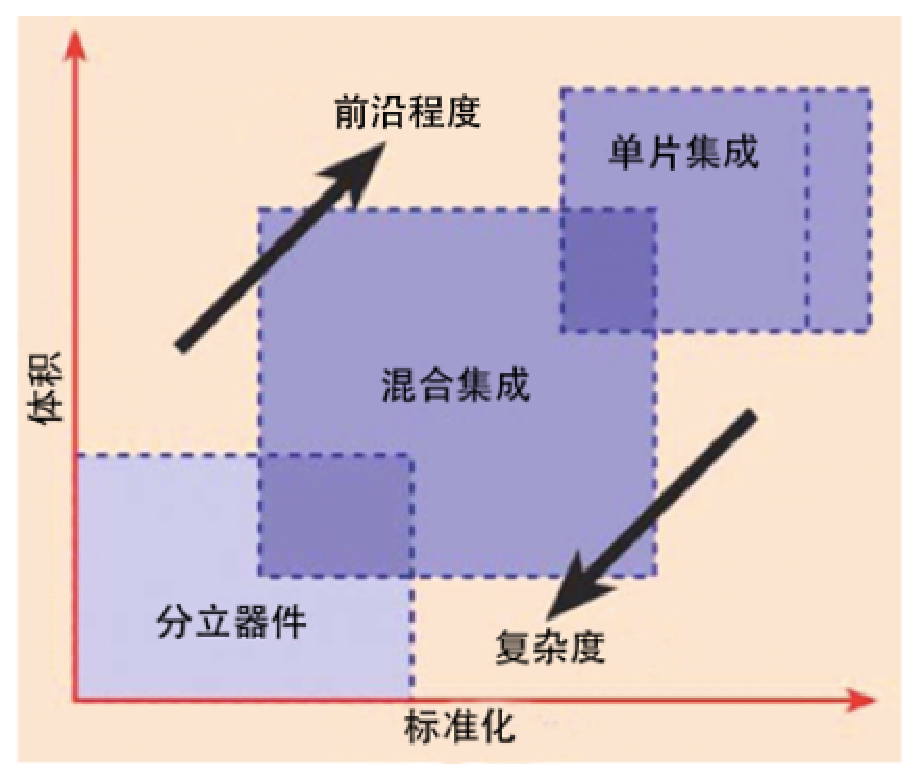
\includegraphics[width=0.5\textwidth]{./Pictures/integrations.eps}\\
  \caption{分立器件、混合集成和单片集成的关系}
  \label{fig_integrations}
\end{figure}

\subsection{混合集成}

2002年,瑞典乌普萨拉大学的Donato Pasquariello和Klas Hjort提出了一种将InP和Si芯片绑定在一起的方法\cite{Pasquariello2002Plasma}。这种方法的关键在于,使用氧气等离子体轰击要绑定的表面,然后进行低温退火。这项技术的发明为InP和Si混合集成的出现铺平了道路。2005年,美国加州大学圣芭芭拉分校的John Bowers教授在其基础上提出了将InP激光器集成在Si波导上的方案\cite{Park2005Hybrid}。最早的混合集成激光器如图~\ref{fig_hybrid}所示。本质上来说,他们采用了InP量子阱和SOI两个芯层,然后进行上下耦合,其原理类似于偏执量子阱结构。那时候的混合集成激光器还是一些简单的FP激光器,而且没有制作电极,需要用光泵浦。随后,他们又成功制作了一系列连续FP激光器\cite{Fang2006A}、电泵浦FP激光器\cite{Fang2006Electrically}、DFB激光器\cite{Srinivasan2011Design}、DBR激光器\cite{Fang2008A}、SGDBR激光器\cite{Sysak2008Integration}、放大器\cite{Sysak2008Integration}、调制器\cite{Kuo2008High}、探测器\cite{Park2007A}~等分立器件。混合集成的一个优点在于,他可以直接利用Si/SOI上面的无源器件,并且可以继承集成电路中的Si工艺为集成光路所用。所以,混合集成可以很容易地将SOI波导和SOI上面的刻蚀衍射光栅、阵列波导光栅等器件集成在光芯片中。

\begin{figure}[htbp]
  \centering
  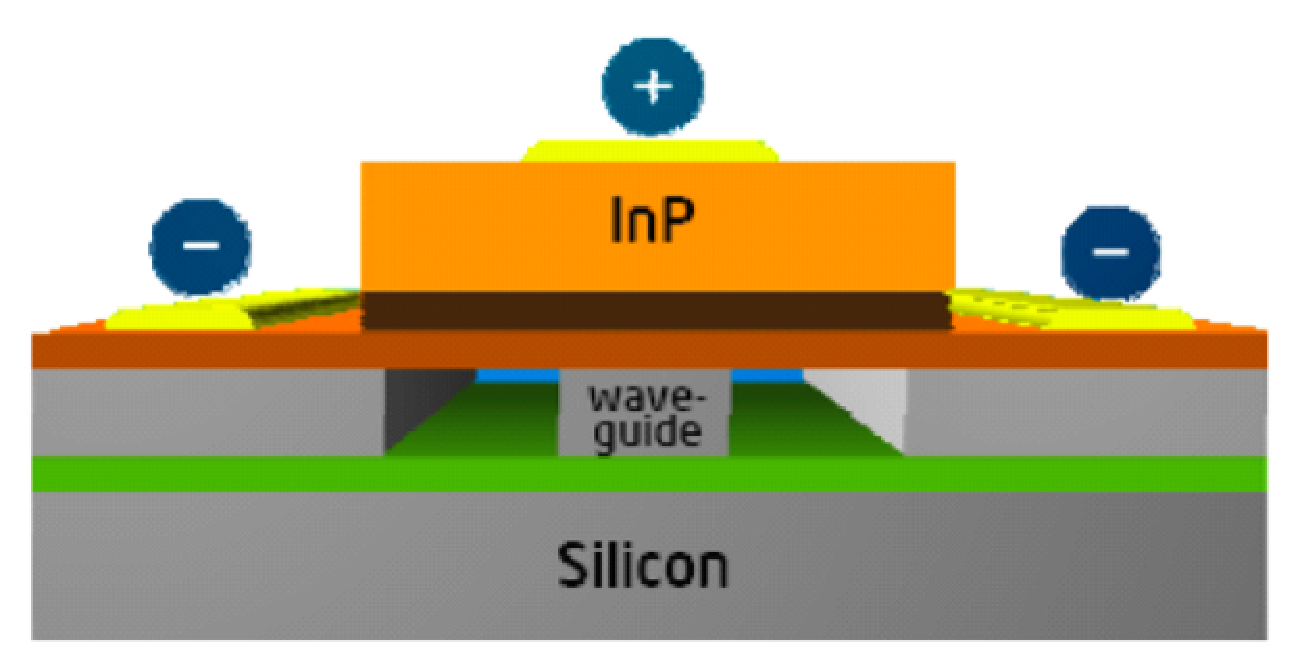
\includegraphics[width=0.7\textwidth]{./Pictures/hybrid.eps}\\
  \caption{SOI脊型波导与III-V有源外延结构绑定的横截面示意图\cite{Park2005Hybrid}}
  \label{fig_hybrid}
\end{figure}

图~\ref{fig_hybrid2}~展示了他们利用现有技术制作的一个四通道稀疏波分复用混合集成的光通信系统\cite{Alduino2010Demonstration}。系统的光发射机由四个DBR激光器、四个行波电极调制器和一个刻蚀衍射光栅组成。其中DBR部分采用了III-V和Si绑定的技术,其他两种器件都是Si上的无源器件。系统的光接收机由一个刻蚀衍射光栅和四个SiGe光探测器构成。激光器的波长被选择为国际电信联盟确定的1291~nm、1311~nm、1331~nm和1351~nm四个标准波长。对于每一个DBR激光器和调制器来说,他们的调制速度可以达到10~Gbps。

\begin{figure}[htbp]
  \centering
  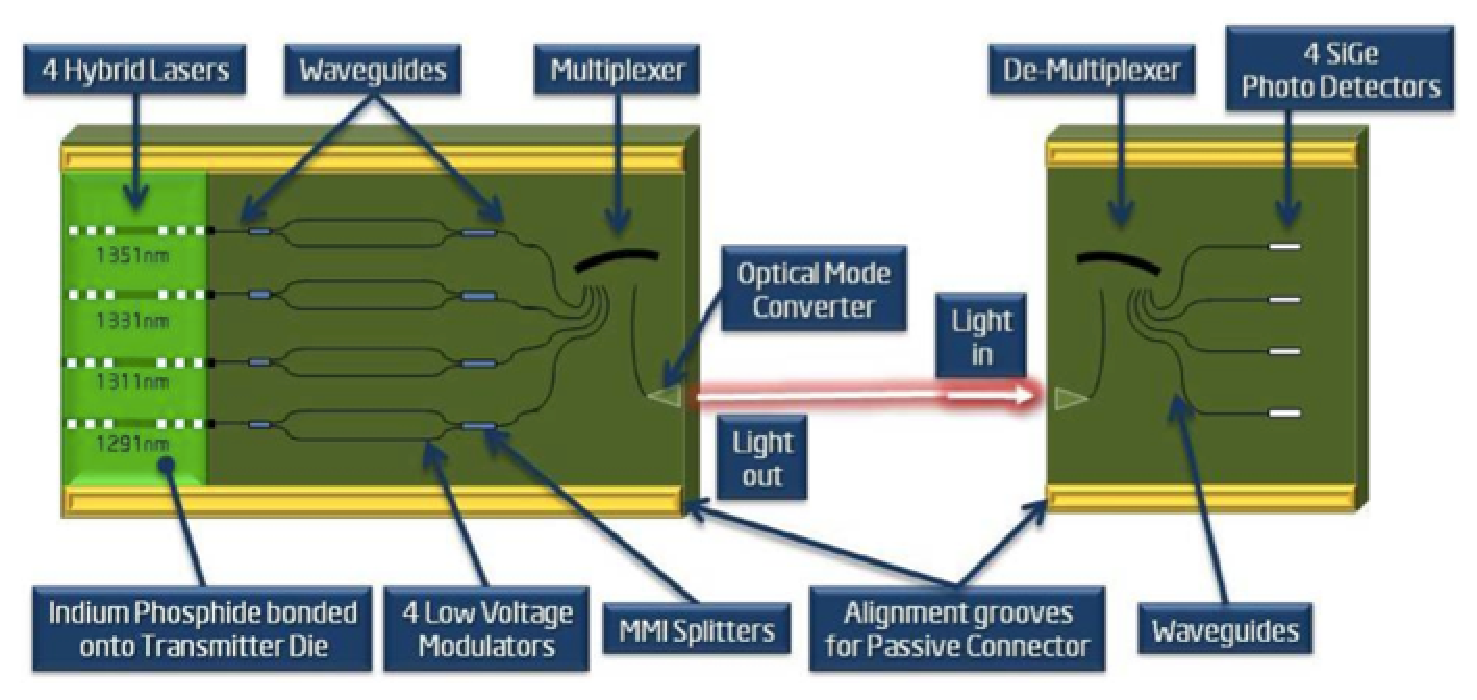
\includegraphics[width=0.7\textwidth]{./Pictures/hybrid2.eps}\\
  \caption{四通道稀疏波分复用混合集成光发射机和光接收机示意图\cite{Alduino2010Demonstration}}
  \label{fig_hybrid2}
\end{figure}

\subsection{单片集成}

单片集成顾名思义,就是将所有的光器件,制作在同一块InP量子阱芯片上。将光通信器件单片集成在同一块芯片上,不仅可以彻底解决耦合的问题,还可以减少封装成本。然而,其缺点是,每个器件必须制作在同一块芯片上,这样做在技术上是很困难的。

在单片集成光通信元器件时,有一些必须满足的要求。首先,每一个集成组件必须实现预期的功能。每一个组件也许不需要像分立器件那样性能好,但是至少也需要达到集成在一起实现整体功能的基本要求。第二个要求是一个组件的操作不会产生不利于另一个器件的影响。每一个组件在一个集成回路中,应当与其他的部件在功能上分离,就好像它是一个分立器件。

已经有一些很好的方法用来生产简单的光子集成回路了。这样的方法包括对接再生长(BJR)\cite{Binsma1997Characterization},选择性区域外延(SAG)\cite{Aoki1993InGaAs},和使用偏置量子阱\cite{Mason1999Widely}等等。首先,对接再生长就是把一部分的波导芯层去掉,再用另一种材料再生长。这个过程中,要精确地刻蚀原来的波导的芯层,然后重新生长的波导材料又要在成分和厚度上与原来的匹配,这是非常困难的。另一种选择性区域外延方法的关键是掩模的选择性生长。在这个过程中,在外延之前需要先在表面生长一层掩模。掩模的形状可以决定外延生长的组分和厚度。在晶片的某些能带,这种方法是有用的,但是在这些区域内由于厚度的变化,光学限制因子就不能被单独优化了。最后,偏置量子阱就是在波导之上的一层量子阱被选择性地除去。这种方法已经成功地被用来制造各种集成芯片\cite{Mason2000Design}\cite{Mason1998Tunable}\cite{Fish1998Compact}。然而,使用偏置量子阱时,整块芯片一般只能制作出两个能带,对于制造复杂的集成光路就束手无策了。量子阱混杂(QWI)\cite{Marsh1993Quantum}方法是一种新型的制作集成光路的方法。他的原理是首先在量子阱片表面产生缺陷,然后在快速热退火的作用下,这层缺陷会往下扩散到量子阱层,促进阱和垒的混杂,达到禁带宽度蓝移的目的。这种方法既不需要对接再生长方法的多次外延,也不需要选择性区域外延的选择性掩膜,所以工艺更加简单,成本更低。

下面介绍两个单片集成光发射机的例子。图~\ref{fig_infinera}~展示了一个100~Gb/s密集波分复用单片集成光发射机,他由美国Infinera公司在2005年提出\cite{Nagarajan2005Large}。整个光发射机由10个DFB、EAM、VOA、OPM和一个阵列波导光栅组成。其中每个激光器可以达到10~Gb/s的调制速率,这样整个发射机的带宽就可以达到100~Gb/s。他们采用了对接再生长这种最可靠的集成方案,将DFB、EAM、VOA和OPM经过多次刻蚀和外延的方法制作出来。

\begin{figure}[htbp]
  \centering
  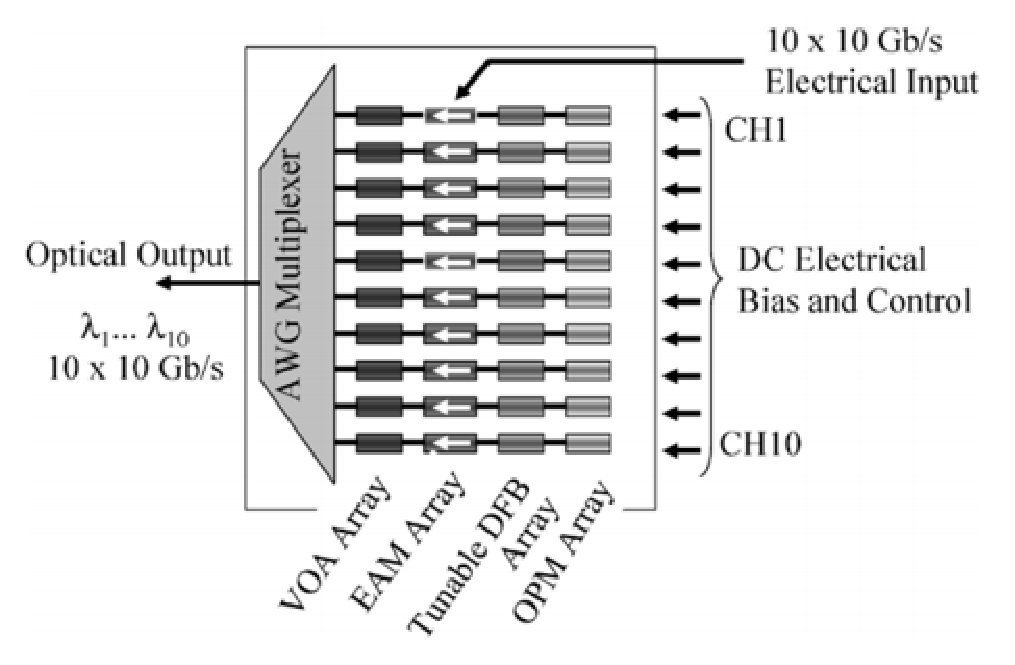
\includegraphics[width=0.7\textwidth]{./Pictures/infinera.eps}\\
  \caption{100Gb/s 密集波分复用大范围集成光路发射机\cite{Nagarajan2005Large}}
  \label{fig_infinera}
\end{figure}

更新一点的方案是一个单片集成可调谐光路由器。美国UCSB大学的Larry Coldren教授团队报道了一个8×8 InP单片集成波长可调路由器\cite{Nicholes2010An},也是当时世界上最复杂的单片集成光器件,如图~\ref{fig_motor}~所示。该器件需要集成8个取样光栅分布式布拉格反射激光器(SGDBR),8个SOA、8个MZI调制器以及1个阵列波导光栅等器件。他们采用了量子阱混杂的方案,将SGDBR的部分区域和MZI等区域进行量子阱混杂处理。在每个器件制作之前,这部分芯片的材料的禁带宽度从原先的1545~nm蓝移到了1420~nm。对于每一个激光器来说,他可以达到40~Gb/s的调制速度。这里使用了可以大范围调谐的SGDBR,并且可以覆盖整个C波段(1530~nm~1562~nm)。所以他可以调谐到C波段的任意波长,并且每个波长的带宽都是40~Gb/s。和Infinera的方案相比,这个芯片的功能更加强大,并且不需要很多次外延来生长有源器件,所以在技术上更胜一筹。但是,由于SGDRB本身比较复杂,无论是制作还是电极控制,都大大增加了复杂度。所以他还处在实验室完善阶段,距离商业化生长还有很长的路要走。但是笔者相信,经过一段时间的完善之后,后者取代前者将是历史的必然选择。

\begin{figure}[htbp]
  \centering
  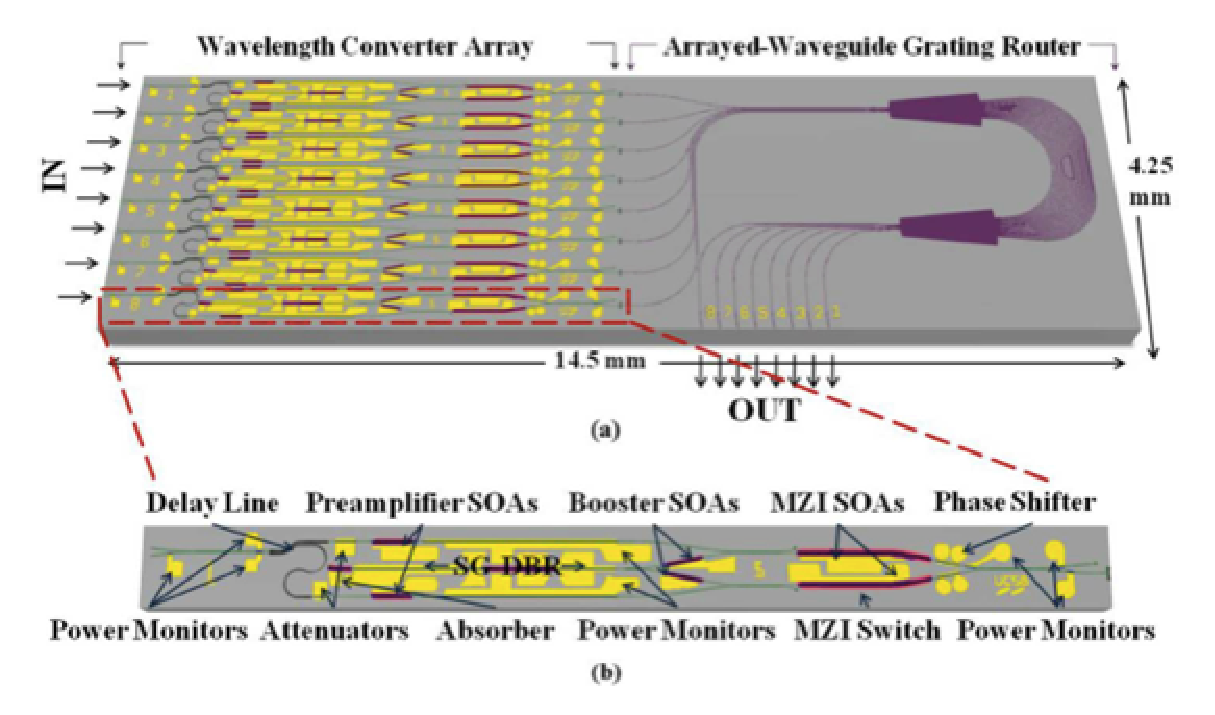
\includegraphics[width=0.7\textwidth]{./Pictures/motor.eps}\\
  \caption{(a)单片集成可调谐光路由器示意图(b)每一个激光器各个部分的细节\cite{Nicholes2010An}}
  \label{fig_motor}
\end{figure}

%%%%%%%%%%%%%%%%%%%%
\section{本文概述}
%%%%%%%%%%%%%%%%%%%%

\subsection{章节安排}
本文的主要工作就是总结InP量子阱混杂的各个方案,详细研究和优化了KrF准分子激光器量子阱混杂技术。基于该技术建立了一个InP单片集成工艺解决方案。并且应用到V型腔激光器中,实现基于载流子注入的波长调谐技术。本文的章节安排如下:

在第二章中,总结了单片集成技术的各个方法以及量子阱混杂技术的各个方案。最后比较了各个方案的优缺点。

在第三章中,介绍了量子阱混杂技术的理论模拟方法,详细阐述了扩散长度和k值对能带蓝移的影响。

在第四章中,介绍了KrF准分子激光器实现量子阱混杂的原理,分析了各个实验参数对实验结果的影响,并制作了激光器、无源波导等分立器件验证该技术的可用性。

在第五章中,介绍了KrF准分子激光器量子阱混杂方法应用到V型腔可调谐激光器中,实现基于载流子注入的波长调谐技术。

最后一章是全文的总结和展望。

\subsection{主要创新点}

(1)在InP量子阱材料上,利用实验室现有的KrF准分子激光器开发了基于紫外激光照射的量子阱混杂技术。利用该技术首次制作了量子阱混杂之后的激光器、无源波导。结果表明,量子阱混杂之后的激光器和波导的性能比混杂之前的还略微提升了。

(2)将KrF准分子激光器量子阱混杂技术应用到V型腔半导体激光器中,首次实现基于载流子注入的波长调谐功能。该激光器可以利用单个电极控制得到1550~nm波段的32个通道100~GHz间隔的连续波长调谐。同时调谐的电流范围是0$\sim$40~mA,和之前的热调谐V型腔激光器相比大大减小了。

(3)进一步发掘了使用KrF准分子激光器量子阱混杂技术之后的V型腔激光器的波长调谐性能。利用长腔和短腔两个电极同时调谐的方法,实现了64个通道100~GHz间隔的波长调谐。

(4)分析了使用KrF准分子激光器量子阱混杂技术之后的V型腔激光器的快速波长切换性能。测试得到相邻通道的波长切换时间可以达到1~ns左右,比热调谐快4个数量级。同时测试了波长切换时间和波长间隔的关系。发现间隔0~10个通道间隔条件下,波长切换时间从1~ns上升到10~ns左右。在11个通道间隔以上的条件下,波长切换时间在稳定10~ns左右,趋于饱和。

%%%%%%%%%%%%%%%%%%%%
\chapter{单片集成技术以及量子阱混杂技术概述}
%%%%%%%%%%%%%%%%%%%%

%%%%%%%%%%%%%%%%%%%%
\section{单片集成技术的要求}
%%%%%%%%%%%%%%%%%%%%

为了实现单片集成的效果,仅仅将各个分立器件制作在同一块芯片上是远远不够的,因为我们需要考虑各个器件的禁带宽度的兼容性。如图~\ref{fig_pic}~所示,当激光器、调制器和无源波导集成在一块芯片上时,我们希望激光器发出的光在调制器中是透明传输的,而当调制器加上合适的电压时又可以吸收激光器的光。同时,无源波导的材料对于激光器的光又是完全透明的。而探测器又可以完全吸收激光器发出的光。由此我们可以推断,为了实现单片集成的效果,我们希望调制器材料的禁带宽度略大于激光器的禁带宽度(差距通常是60~nm左右),同时无源波导的禁带宽度远大于激光器的禁带宽度(差距通常在100~nm以上),最后探测器的禁带宽度小于激光器的禁带宽度。从制作工艺的角度来说,我们需要将半导体芯片在水平方向分成不同的区域,并且非常精确地将每个区域的材料的禁带宽度控制在特定波长上,然后在各个区域制作不同的器件。举例来说,对于图~\ref{fig_pic}~的器件,如果把他看做一个用于光通信的光发射机芯片,那么我们需要将整块芯片分成激光器,调制器、无源波导和探测器四个区域。激光器的波长应该准确的位于1550~nm,那么调制器的禁带宽度对应的波长应该在1490~nm左右,无源波导的禁带宽度对应的波长应该小于1450~nm,探测器的禁带宽度对应的波长应该大于或等于1550~nm。

\begin{figure}[htbp]
  \centering
  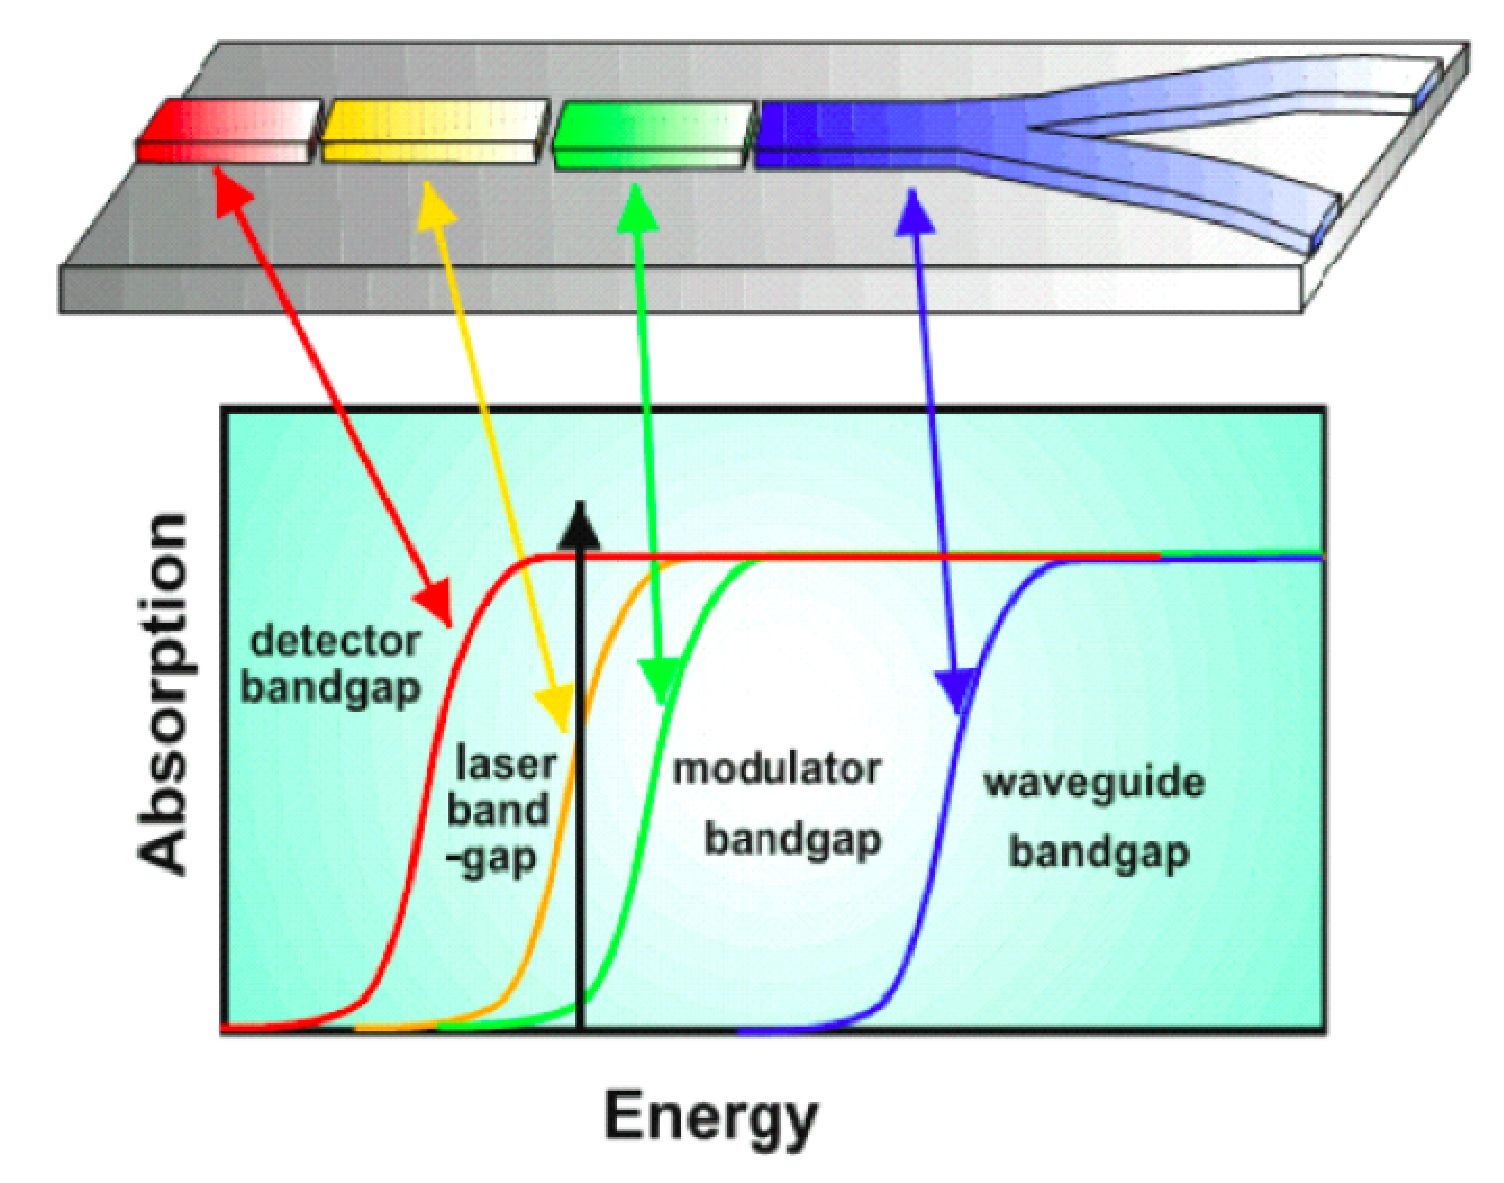
\includegraphics[width=0.5\textwidth]{./Pictures/pic.eps}\\
  \caption{光子集成回路示意图}
  \label{fig_pic}
\end{figure}

总的来说,任何一种单片集成的方法至少需要达到以下几条要求:

\begin{enumerate}
\item{精确的改变每个分立器件的材料的禁带宽度}
\item{空间分辨率应该远小于器件的尺寸}
\item{材料的其他特性不能变差太多,比如折射率、损耗、电特性等}
\end{enumerate}

%%%%%%%%%%%%%%%%%%%%
\section{单片集成技术的方法}
%%%%%%%%%%%%%%%%%%%%

为了在一块芯片上做出不同的禁带宽度,在过去的几十年中,已经有很多种方法实现这样的效果。然而,每一种方法都有他的优点和缺点,所以在实际生产中,还没有形成一种通常的解决方案,这也是该领域值得研究的一个问题。图~\ref{fig_pic_methods}~例举了几十年来人们所研究的各种单片集成方法。

\begin{figure}[htbp]
  \centering
  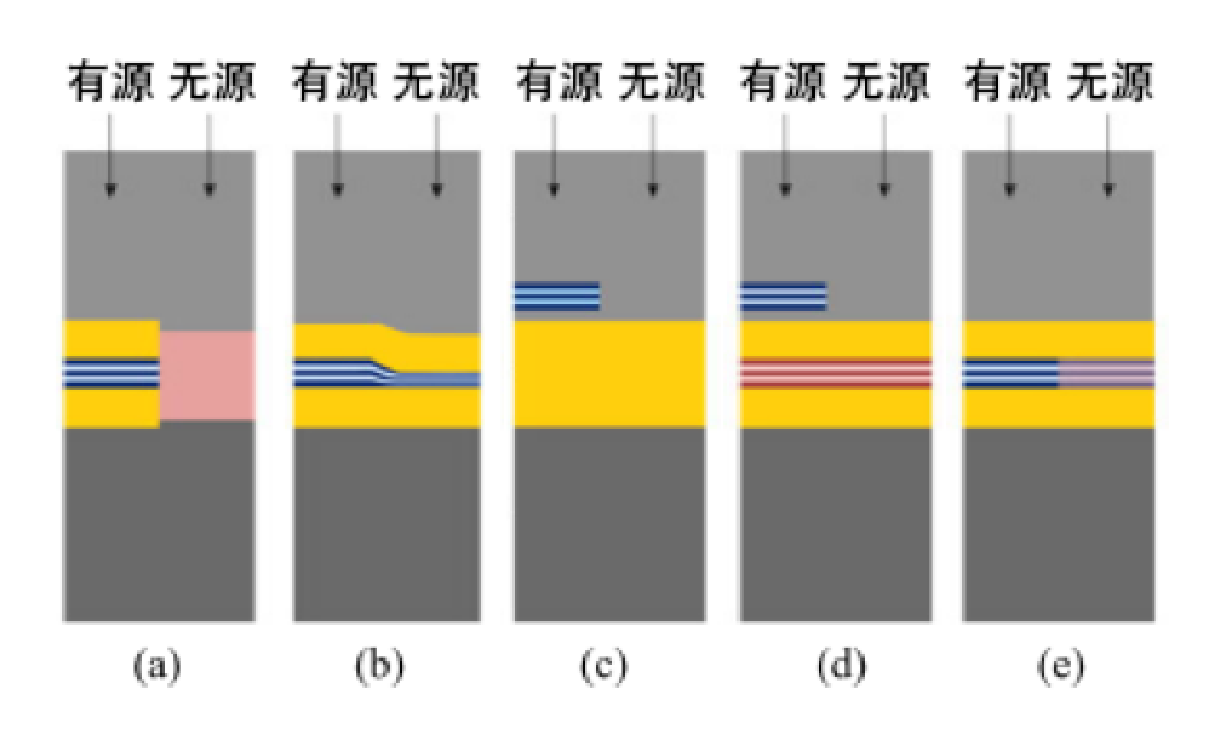
\includegraphics[width=0.7\textwidth]{./Pictures/pic_methods.eps}\\
  \caption{有源和无源器件单片集成的各种方法}
  \label{fig_pic_methods}
\end{figure}

%%%%%%%%%%%%%%%%%%%%
\subsection{对接再生长}
%%%%%%%%%%%%%%%%%%%%

对接再生长的方法如图~\ref{fig_pic_methods}~(a)所示。这种方法的原理是,首先生长一片全部包含有源层的芯片,然后将无源部分的芯层刻蚀掉,最后在这些地方重新生长无源的芯层和包层。这种方法的优点是,每个部分的材料禁带宽度都可以非常准确的控制。同时,它的缺点也是显而易见的。由于有源的芯层和无源的芯层必须对准,而通常的量子阱片芯层仅有几十纳米,所以这给工艺带来了不小的难度。此外,如果需要制作多种不同禁带宽度的材料,就需要进行多次的刻蚀和再生长,大大增加了工艺的复杂度。最后,由于之后生长上去的材料和原先的材料完全不同,所以很可能存在较大的折射率差,这样会导致界面上的光被反射,增加了额外的损耗。近年来,很多人通过改进工艺,大大减小了界面的反射率,但是界面的质量依然是工艺上的难点。总而言之,这种方法最直接、最有效,同时在工艺上的难度和复杂度限制了它的发展。

%%%%%%%%%%%%%%%%%%%%
\subsection{选择性区域生长}
%%%%%%%%%%%%%%%%%%%%

选择性区域生长的方法如图~\ref{fig_pic_methods}~(b)所示。这种方法只需要一步生长就可以完成,所以是对对接再生长的改进。这种方法的原理是,在芯片生长芯层之前,先在芯片上生长一层介质膜。然后,在用金属氧化物化学气相沉积(MOCVD)生长芯层的过程中,由于介质膜的影响,材料的厚度和组分会发生变化,导致禁带宽度的改变。只要介质膜生长得当,这种方法可以一次性生长出多个需要的禁带宽度的材料。不过,这种方法对MOCVD生长条件的控制非常苛刻,所以工艺难度非常高,同时器件的性能很容易受到表面状态的影响。

%%%%%%%%%%%%%%%%%%%%
\subsection{偏置量子阱}
%%%%%%%%%%%%%%%%%%%%

图~\ref{fig_pic_methods}~(c)是偏置量子阱方法。这种方法的原理是,有源层的芯层被生长在无源层的芯层之上,最后在无源区域刻蚀掉有源层的芯层。这种方法比较简单直接,但是缺点似乎更多。首先,它只能将两种禁带宽度的器件集成在一起。然后,由于有源芯层不在最中间,激光器的限制因子会大大下降,这样会大大减小激光器的增益。最后,无源部分不包含量子阱层,所以在制作调制器时,性能会有所折扣。

%%%%%%%%%%%%%%%%%%%%
\subsection{双量子阱}
%%%%%%%%%%%%%%%%%%%%

图~\ref{fig_pic_methods}~(d)是双量子阱方法。显然,该方法是偏置量子阱方法的改进。它在偏置量子阱的基础上,在无源芯层也生长了量子阱。这样可以解决调制器的性能问题。可是这种方法并不能解决偏置量子阱方法的其他问题,例如激光器限制因子仍然比较低等等。同时,由于无源区域包含量子阱层,损耗也要比偏置量子阱大很多。

%%%%%%%%%%%%%%%%%%%%
\subsection{量子阱混杂技术}
%%%%%%%%%%%%%%%%%%%%

从制作工艺的角度来说,图~\ref{fig_pic_methods}(e)所示的量子阱混杂技术可能是最简单的单片集成方法。如图~\ref{fig_qwi}~所示,对于普通的量子阱材料来说,沿着材料的生长方向看过去,每一层材料的禁带宽度是一种矩形的结构。整个量子阱的禁带宽度是由阱的材料和厚度,以及垒的材料决定的。然后,当我们通过某种方法,将阱和垒的材料进行融合,使量子阱的每一层的禁带宽度变成一个渐变的结构之后,整个材料的禁带宽度就会发生变化(通常是禁带宽度增加)。所以,我们只需要在芯片生长完之后,制作各个部分的器件之前,对调制器和无源波导等区域进行量子阱混杂,其中禁带宽度的变化量由混杂的工艺参数决定,这样就可以实现单片集成的效果。

\begin{figure}[htbp]
  \centering
  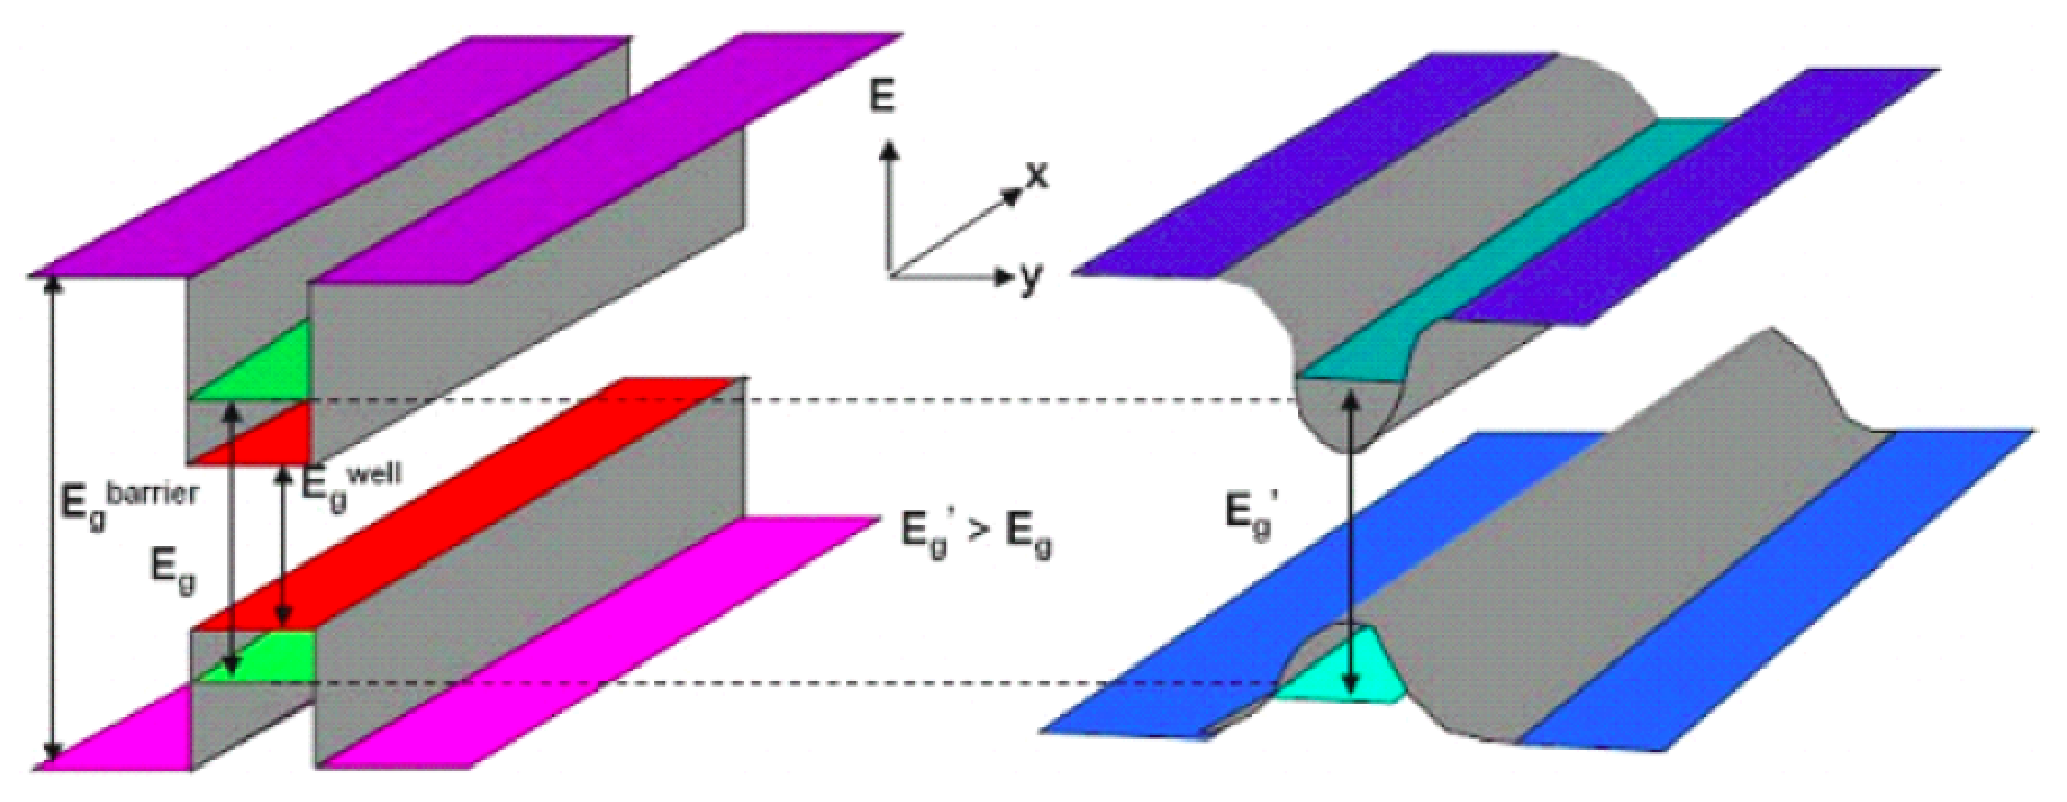
\includegraphics[width=0.7\textwidth]{./Pictures/qwi.eps}\\
  \caption{量子阱混杂技术示意图}
  \label{fig_qwi}
\end{figure}

为了让阱和垒互相融合,高温退火是最直接的方法。然而,只做退火的方法会引起一整片材料的禁带宽度变化,我们需要的是在特定的区域内改变材料的禁带宽度。所以通常会在芯片特定区域的表面或者内部产生一些缺陷。这些缺陷在快速退火的条件下,可以快速扩散到量子阱层,引起阱和垒互相扩散,达到量子阱混杂的目的。这些缺陷同时还能起到促进阱和垒互相扩散的目的,和单纯使用退火的方法相比,退火温度要低得多,退火时间要短得多。

除了快速热退火和引入的缺陷会影响量子阱混杂的效果之外,量子阱本身的结构也起到很大的作用。2009年,墨西哥INAOE研究院、瓜纳华托大学和美国佛罗里达大学共同发表了一篇关于InP量子阱结构对混杂的影响的文章\cite{May2009Intermixing}。文章中采用了InGaAsP/InGaAsP、InGaAs/InGaAsP和InGaAs/InP三种不用的量子阱结构,在相同的实验条件下比较他们的混杂效果,如图~\ref{fig_layers}~所示。结果显示,量子阱的材料对蓝移的大小起了非常大的作用。InGaAs/InP量子阱因为阱和垒只有In原子是相同的,所以两种材料的差异最大,最容易达到量子阱混杂的效果。InGaAs/InGaAsP量子阱有In、Ga和As三种元素是共有的,所以混杂效果比前者差很多。而InGaAsP/InGaAsP的元素完全相同,只有组分不同,所以总体来说比InGaAs/InGaAsP量子阱的效果更差一些。

\begin{figure}[htbp]
  \centering
  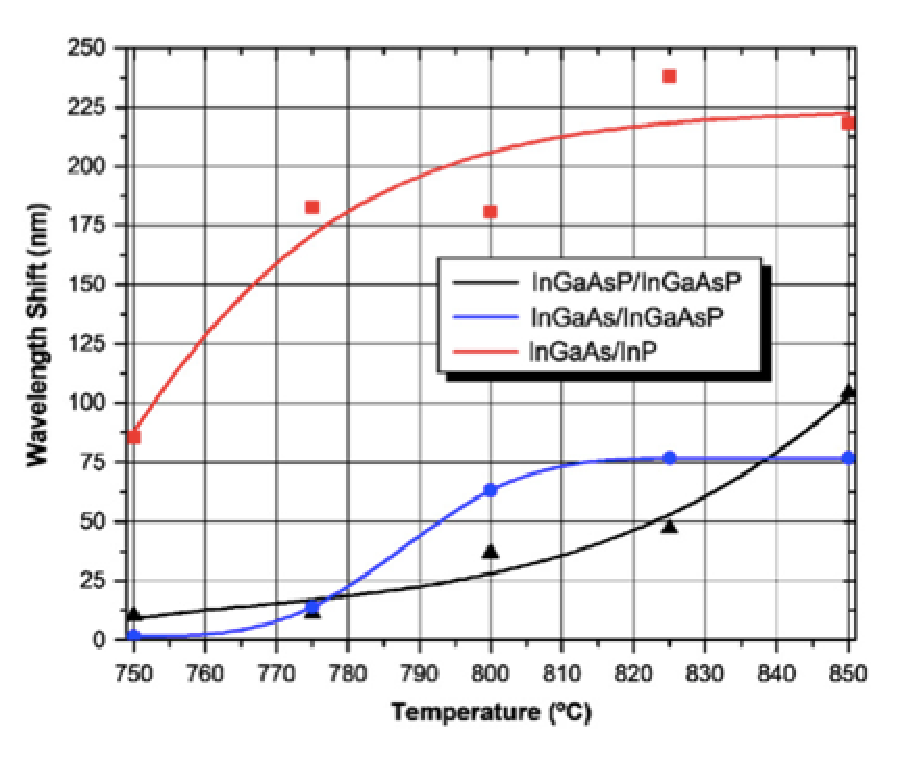
\includegraphics[width=0.7\textwidth]{./Pictures/layers.eps}\\
  \caption{InGaAs/InGaAsP、InGaAs/InGaAsP和InGaAs/InP量子阱混杂后的蓝移随温度的变化曲线}
  \label{fig_layers}
\end{figure}

由于条件有限,我们在实验中采用的量子阱结构都是同一种,即InGaAsP/InGaAsP量子阱。 这是一个1.2\%压应变的应变五量子阱结构,激射波长在1550~nm左右。从上到下,依次包含0.5~μm厚的InP牺牲层,0.2~μm厚的InGaAs盖层,1.5~μm厚的InP上包层,0.004~μm厚的InGaAsP阻刻层,渐变折射率层,五量子阱层,渐变折射率层,最下面是InP基片。在本文的后面篇章中,我们不会通过改进量子阱结构来提升量子阱混杂的效果。参考前面的讨论,InGaAsP/InGaAsP量子阱是相对来说效果最差的一个组合,这里还有很大的提升空间。

量子阱混杂的一个优点在于,该方法是在芯片外延之后进行的,所以只需要进行一次外延生长。该技术的具体实现方案通常是比较容易实现的,所以工艺复杂度比较低。此外,该方法制作的器件的性能也比较好。由于量子阱混杂之后,材料性能的变化很小,例如折射率基本不变,这样就不会在有源和无源区域的边界引入额外的损耗。该技术的缺点在于,具体的实现方案往往缺乏稳定性,在工艺参数发生微小变化的情况下,量子阱混杂的效果可能会发生较大变化。为了能得到稳定可靠的量子阱混杂技术,人们还在不断的创造和完善之中。

%%%%%%%%%%%%%%%%%%%%
\subsection{各种单片集成技术的比较}
%%%%%%%%%%%%%%%%%%%%

表~\ref{integration_compare}~比较了各种单片集成方法的优缺点,仅供参考。
\begin{table}[htbp]
    \zihao{5}
    \caption{各种单片集成方法的优缺点}
    \centering
    \label{integration_compare}
    \begin{tabular}{cccccc}
        \hline
        \hline
                   & 对接再生长 & 选择性区域生长 & 偏置量子阱 & 双量子阱 & 量子阱混杂\\
        \hline
        单次外延    &  否       & 是           & 否        & 否      &是\\
        工艺复杂度   &高        &高             &高        &高       &低\\
        能带数量    &多个       &多个           &2个       &2个       &多个\\
        稳定性      &好        &好             &好        &好        &中\\
        \hline
        \hline
    \end{tabular}
\end{table}

%%%%%%%%%%%%%%%%%%%%
\section{量子阱混杂技术回顾}
%%%%%%%%%%%%%%%%%%%%

量子阱混杂是一个量子阱的阱和垒相互扩散的过程。在这个过程中,随着扩散的不断增强,量子阱的形状和厚度也随之不断变化,从而导致能带的变化。变化之后的能带对应的能量一般来说都是增加的,也就是波长发生蓝移。在一般情况下,量子阱的阱和势垒之间的界面是亚稳态的,在一定的条件下,例如高温下,量子阱的阱和势垒的原子会相互扩散。量子阱混杂的目标不是简单地使阱和势垒相互扩散,而是在整个区域中做选择性的扩散。

已经有很多种方法可以实现量子阱混杂的效果,例如杂质诱导无序(IID) \cite{holonyak1998impurity} ,无杂质空位增强无序(IFVD) \cite{si1998area},光吸收诱导无序(PAID) \cite{mckee1997monolithic},离子注入增强扩散\cite{charbonneau1998photonic}等等。本节将介绍最近几十年中研究过的绝大部分方法,并进行比较。

%%%%%%%%%%%%%%%%%%%%
\subsection{杂质诱导方法}
%%%%%%%%%%%%%%%%%%%%

19世纪80年代,人们开始研究量子阱混杂技术,第一个被想到和实现的是杂质诱导方法。1981年,美国伊利诺斯大学的W.~D.~Laidig等人提出了使用Zn扩散到AlAs-GaAs超晶格中引起混杂的方法\cite{laidig1981disorder},这也是第一次报道的杂质诱导方法(更详细的介绍可以参考一份相关的专利\cite{holonyak1983method})。如图~\ref{fig_iid}~所示,在AlAs-GaAs超晶格的中间10~um区域,已经有Zn原子扩散到里面,扩散的温度仅仅需要575摄氏度,大大低于GaAs材料本身发生混杂的温度。在Zn扩散进去之后,AlAs-GaAs超晶格的组分发生了变化,变成了AlGaAs的三元合金,材料的禁带宽度也随之增加了。在这个实验中,为了达到Zn原子选择性扩散的目的,芯片表面利用光刻技术覆盖了一层Si$_3$N$_4$掩膜,然后和ZnAs$_2$一起放入专门的扩散炉中,在500$^{\circ}$C$\sim$600$^{\circ}$C的条件下等待10分钟$\sim$60分钟,就可以在没有覆盖Si$_3$N$_4$的地方达到混杂的效果。

\begin{figure}[htbp]
  \centering
  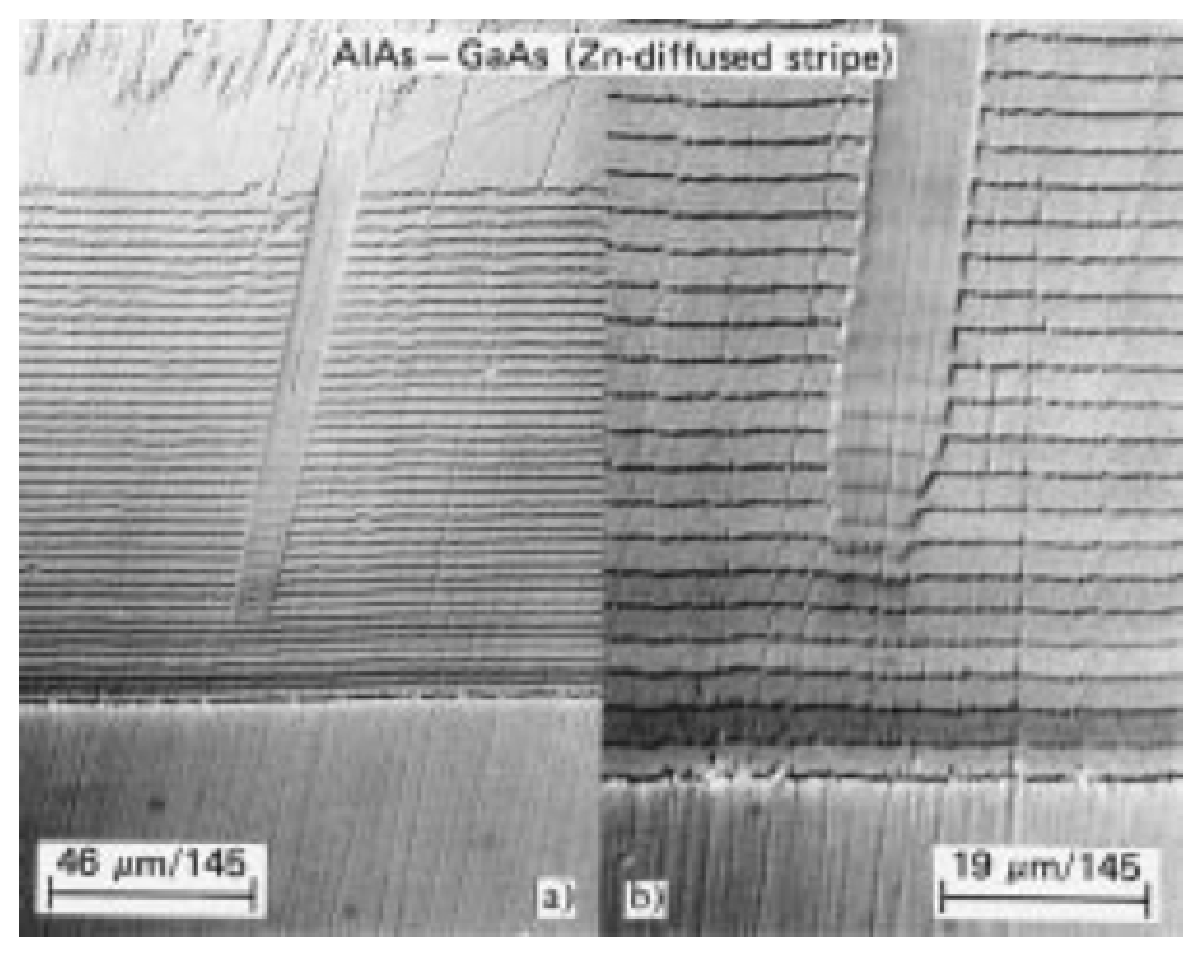
\includegraphics[width=0.7\textwidth]{./Pictures/iid.eps}\\
  \caption{Zn扩散到AlAs-GaAs超晶格中引起混杂的电镜图片}
  \label{fig_iid}
\end{figure}

此后,人们在这篇文章的基础上,对杂质诱导方法进行了大量研究和改进。例如,美国罗克韦尔国际微电子研究发展中心的J.~J.~Coleman等人提出了用低能的Si离子注入实现AlAs-GaAs超晶格混杂的方法\cite{Coleman1982Disorder}。他们使用375keV能量的Si离子,注入到AlAs-GaAs超晶格芯片的表面,然后在退火的作用下,达到了混杂的目的。此后,人们发现了Ge,S,Sn,Se,Be,Mg等原子也可以达到杂质诱导混杂的目的。1984年,美国麻省理工学院在InGaAsP量子阱材料上也实现了杂质诱导混杂的效果。他们用这种方法制作了10GHz的激光器和调制器集成的器件\cite{Tsang1981Intracavity}。然而,这种方法也有一些缺陷,比如电特性并不理想。由于量子阱混杂的过程中需要引入额外的杂质,这些杂质运动到芯片的接触层和上包层之后会使得电特性变差。所以这种方法并不是很适合制作一些复杂的有源器件。因此,人们探索了不使用额外杂质达到量子阱混杂目的的方法,后面介绍的方法都是属于不引入额外杂质的方法。

%%%%%%%%%%%%%%%%%%%%
\subsection{无杂质空位诱导方法}
%%%%%%%%%%%%%%%%%%%%

1986年,美国伊利诺斯大学的L.~J.~Guido等人发现了在GaAs量子阱材料表面的生长介质层会引起光谱蓝移的效果。他们是最早一批发现这种方法实现量子阱混杂的人。他们的实验过程是如图~\ref{fig_ifvd}~所示,首先在GaAs量子阱芯片的表面生长一层SiO$_2$介质层,然后在800$^{\circ}$C$\sim$900$^{\circ}$C之间进行快速热退火。他们发现,GaAs表面的Ga原子由于在SiO$_2$中扩散系数很大,所以会在快速热退火的过程中被吸附上去,这样就会在GaAs表面产生Ga空位。这些空位在随后的快速热退火会继续往下运动到量子阱层,促进阱和垒的扩散,达到量子阱混杂的目的。这种方法与前面的方法相比,由于不需要额外的杂质参与,所以理论上对材料的性能影响更小。同时介质层只需要利用普通的PECVD等设备就可以生长,这也是光器件的标准工艺步骤。

\begin{figure}[htbp]
  \centering
  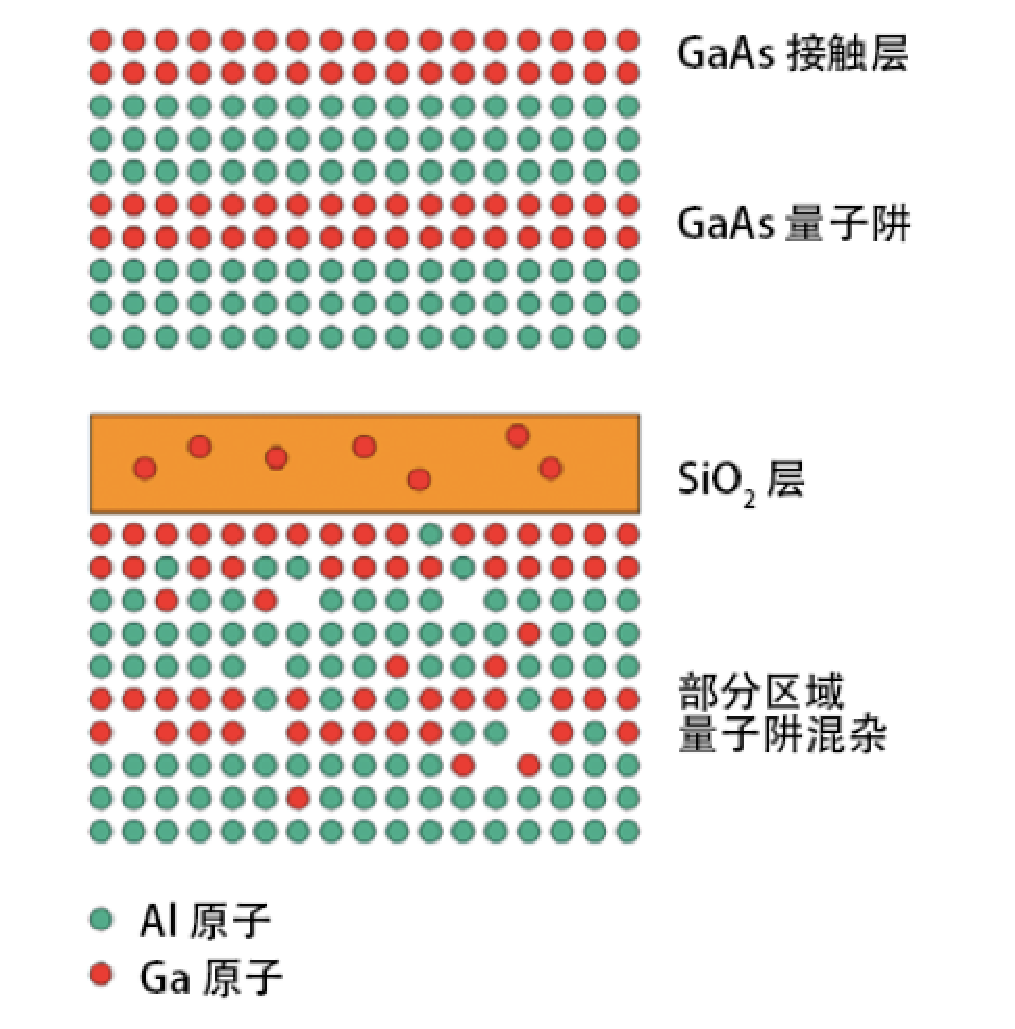
\includegraphics[width=0.5\textwidth]{./Pictures/ifvd.eps}\\
  \caption{(a)原生GaAs量子阱结构,(b)无杂质空位诱导量子阱混杂之后的结构}
  \label{fig_ifvd}
\end{figure}

在GaAs量子阱材料上取得成功之后,人们尝试在InP量子阱材料上重复这个实验。由于必须有Ga原子的参与,介质层生长在InP牺牲层上面并不会达到量子阱混杂的目的,所以必须在InGaAs电接触层上生长。不过这并不是这个方法的真正难点。难点在于,为了将Ga原子吸附到介质层中,必须采用较高的退火温度,通常在800$^{\circ}$C以上。这个温度条件小于GaAs量子阱本身混杂的温度,但是大于InP量子阱本身混杂的温度。其中的一个比较通用的解决办法例如在2002年,J.~H.~Teng等人提出了利用生长Si$_x$N$_y$介质层抑制高温退火带来的蓝移的技术\cite{Teng2002Controlled},结果如图~\ref{fig_ifvd2}~所示。对于生长SiO$_2$的样品,PL波长峰值蓝移到了1390~nm左右,这个蓝移效果是比较理想的。但是,没有介质层的裸片退火之后波长在1500~nm附近,相对于原生片的1575~nm蓝移了75~nm,这个蓝移明显太大。而生长Si$_x$N$_y$部分的蓝移减小到了50~nm以下,明显对混杂起到了抑制作用。他们用这种方法制作了延长腔激光器,达到了10~nm的电调谐范围,这个结果是很理想的。

\begin{figure}[htbp]
  \centering
  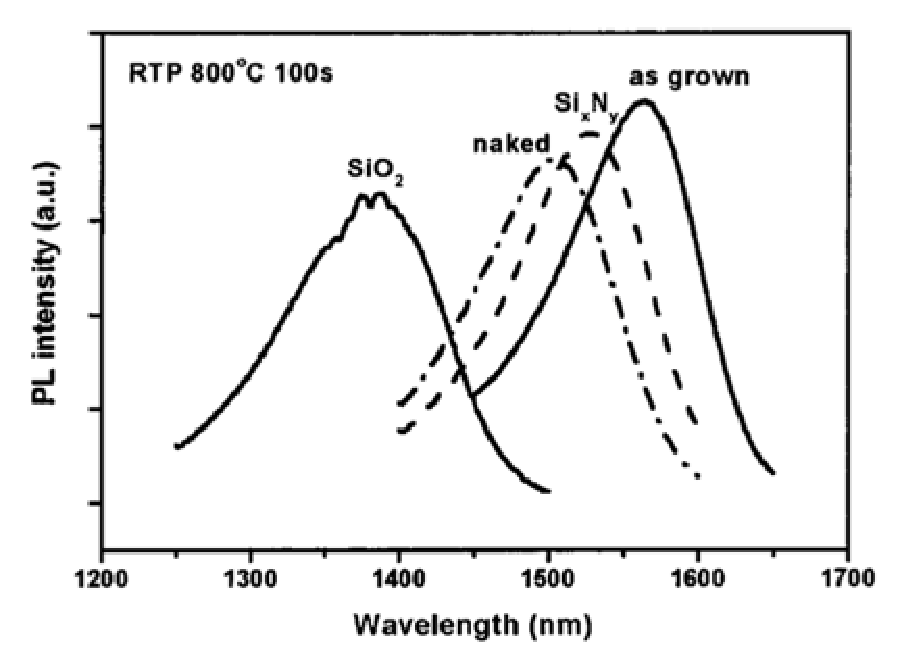
\includegraphics[width=0.7\textwidth]{./Pictures/ifvd2.eps}\\
  \caption{InP量子阱芯片表面生长不同介质层,快速热退火之后测试得到的光致发光谱}
  \label{fig_ifvd2}
\end{figure}

总的来说,这种方法更适合于GaAs量子阱材料,可以说是GaAs量子阱混杂的最佳选择。然而在InP量子阱材料上,需要额外生长抑制蓝移的介质层,给工艺带来了很大的复杂性。所以该技术并不太适合InP量子阱材料。值得一提的是,利用这项关键技术,英国格拉斯哥大学的John~H.~Marsh教授创办了Intense公司,专门生产大功率GaAs半导体激光器。对于GaAs量子阱激光器来说,由于量子阱中Al元素的存在,当注入电流比较大的时候,激光器的端面会突然发生烧毁的现象,导致整个激光器失效。这个现象成为光学灾变(COD)\cite{Sanayeh2006Investigation}。所以GaAs量子阱激光器往往不能输出很大的功率。解决这个问题的一个巧妙的办法就是将靠近解理面部分的材料变成无源材料,形成一个非吸收腔镜(NAM),这样可以很大程度上抑制光学灾变现象的发生,从而提高了GaAs激光器的功率。这也是量子阱混杂技术在激光器中的一个巧妙的应用。

%%%%%%%%%%%%%%%%%%%%
\subsection{低温生长InP方法}
%%%%%%%%%%%%%%%%%%%%

2000年,加拿大McMaster大学的David~Thompson等人提出了一种在InP量子阱芯片上利用低温生长InP和快速热退火实现量子阱混杂的方法\cite{Author2000New}\cite{Lee2000Enhanced}。其中的关键技术在于,他们把量子阱芯片的InP牺牲层的生长温度从470$^{\circ}$C下降到300$^{\circ}$C,这样可以在牺牲层中引入缺陷。这些缺陷在之后的快速热退火中会往下运动,促进阱和垒的混杂,达到禁带宽度蓝移的目的。图~\ref{fig_ltinp}~给出了常温和低温InP层在725$^{\circ}$C快速热退火条件下产生的蓝移随着退火时间的变化趋势。显而易见的是,常温InP层并不会对量子阱混杂达到促进作用,而低温InP层大大促进了量子阱混杂,并且蓝移可以达到170~nm以上。

\begin{figure}[htbp]
  \centering
  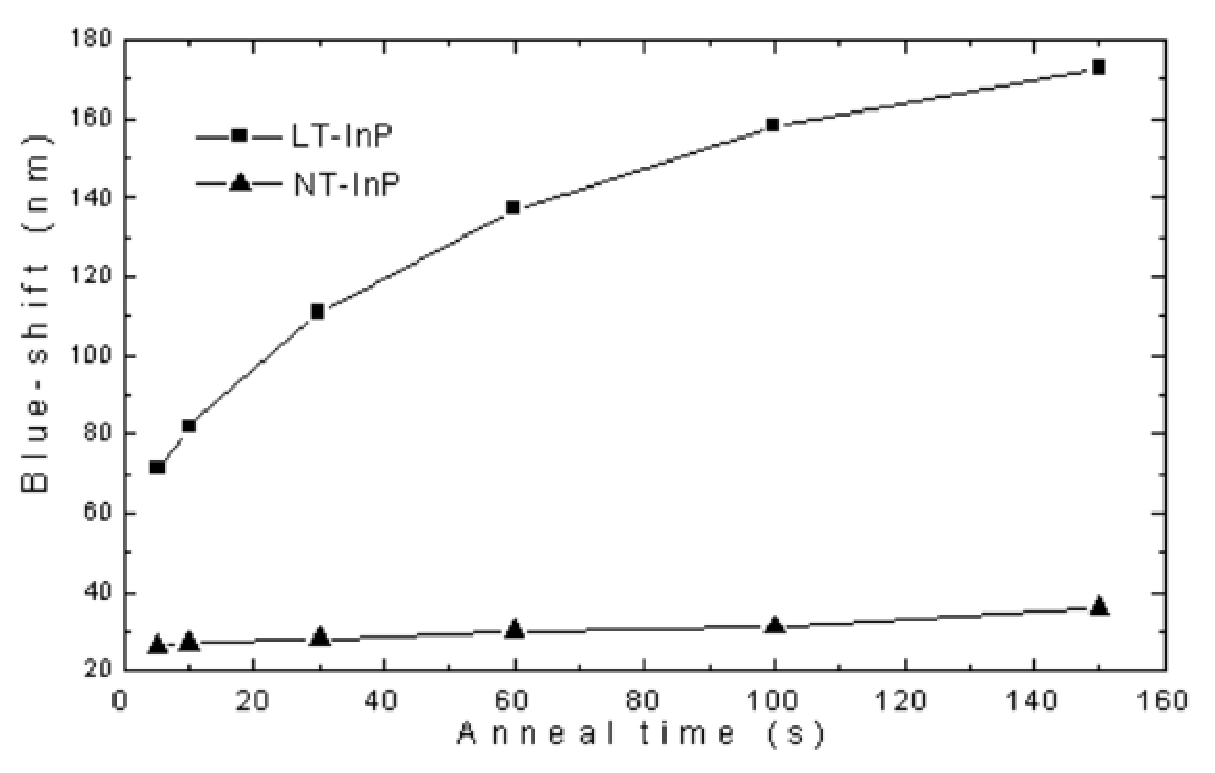
\includegraphics[width=0.7\textwidth]{./Pictures/ltinp.eps}\\
  \caption{常温和低温InP层725$^{\circ}$C快速热退火条件下的蓝移随着退火时间的变化趋势}
  \label{fig_ltinp}
\end{figure}

该课题组在之后的时间里继续探索了这种技术的一些细节问题,包括利用x射线分析量子阱混杂之后的样品组分\cite{Lee2001Enhanced},研究低温生长InP的温度、P流量和厚度对量子阱混杂的影响\cite{Gordon2003Quantum},利用XTEM和EDX技术分析量子阱混杂之后的样品组分\cite{Hulko2006Quantitative},同时衍生出了利用He辅助生长InP\cite{Zhang2003Quantum}和生长InAsP\cite{Hulko2009Quantum}的技术实现量子阱混杂的方法。然而,这种技术并没有往更深的方向发展。由于低温生长InP的工艺本身并不是标准工艺,所以他的可重复性是存在问题的。至今并没有其他的第二个课题组重复过这种技术。他们也没有进一步利用这种技术制作器件。

%%%%%%%%%%%%%%%%%%%%
\subsection{阳极氧化诱导方法}
%%%%%%%%%%%%%%%%%%%%

1998年,香港大学的Shu~Yuan等人提出了一种在GaAs量子阱芯片上采用阳极氧化实现量子阱混杂的方法\cite{Yuan1998Anodic}\cite{Yuan1998Anodic2}。其工艺设备如图~\ref{fig_oxide}~所示。首先,GaAs量子阱片被固定在一个开路的50伏脉冲式电源的阳极上。阳极和阴极之间通过导电液传到电流。导电液由乙二醇、磷酸和去离子水用40:20:1的体积比配制而成。芯片的一半由导热胶覆盖,这样一来,只有另一半暴露在导电液中的部分会被氧化。经过几分钟的脉冲电流处理之后,芯片又进行了快速退火处理。最终的测试结果如图~\ref{fig_oxide_pl}~所示。在芯片没有被氧化的部分,光致发光谱的峰值波长仅仅蓝移了5~meV左右,同时强度下降到只剩原来的1/20。而对于氧化过的部分,蓝移达到了44meV,而强度上升到了原来的两倍多。可见,这种方法在获得较大蓝移的同时,还可以增加光致发光谱的强度。

\begin{figure}[htbp]
  \centering
  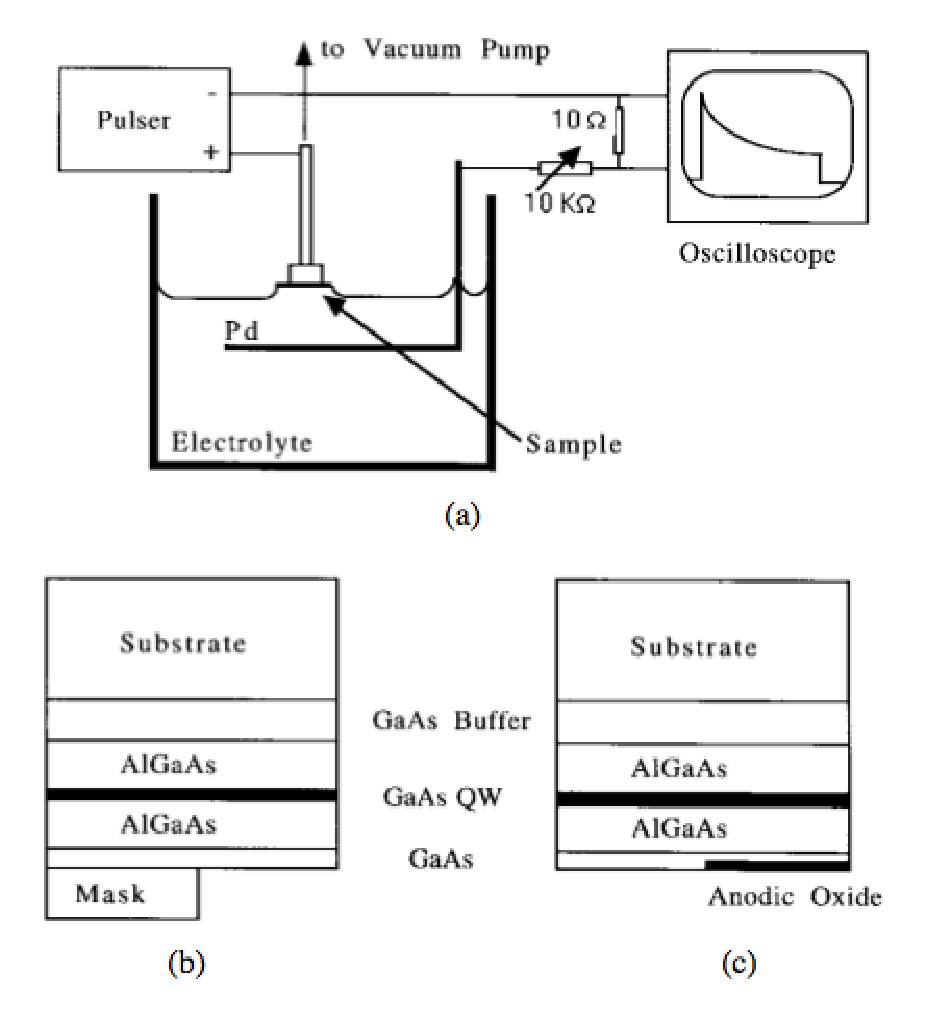
\includegraphics[width=0.5\textwidth]{./Pictures/oxide.eps}\\
  \caption{阳极氧化诱导量子阱混杂技术的设备示意图}
  \label{fig_oxide}
\end{figure}

\begin{figure}[htbp]
  \centering
  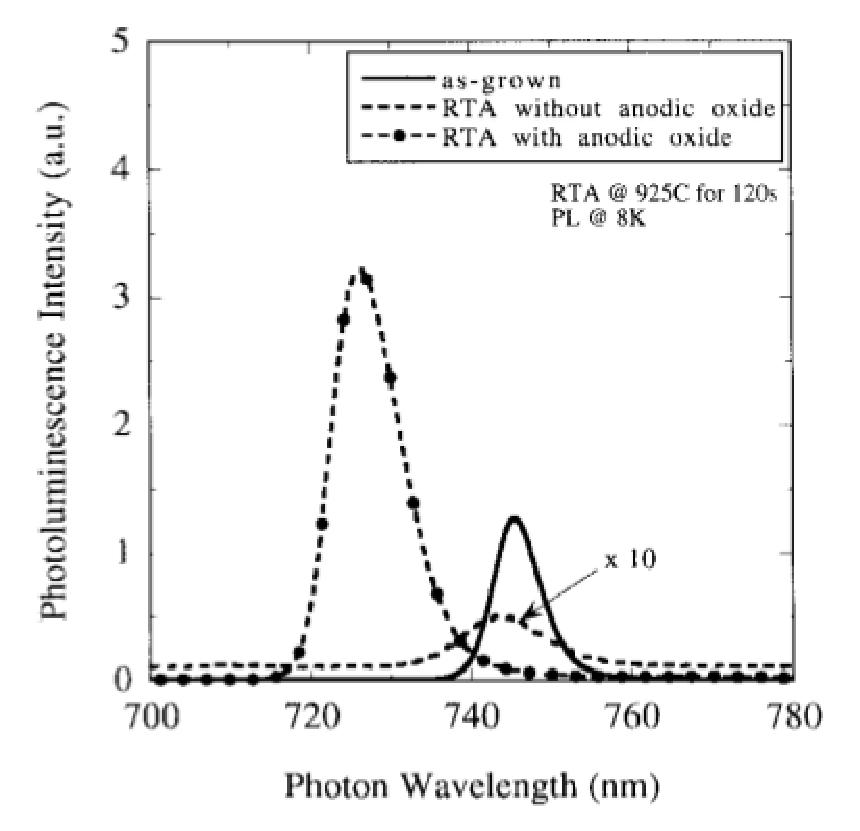
\includegraphics[width=0.5\textwidth]{./Pictures/oxide_pl.eps}\\
  \caption{混杂前后的光致发光谱测试结果}
  \label{fig_oxide_pl}
\end{figure}

可惜的是,这种方法由于需要非常特殊的实验条件,后来并没有进行广泛研究。这种方法也只能停留在研究光致发光谱蓝移的方向上,并没有应用到任何器件上,也没有在InP量子阱材料上成功实现。

%%%%%%%%%%%%%%%%%%%%
\subsection{光吸收诱导方法}
%%%%%%%%%%%%%%%%%%%%

1997年,英国格拉斯哥大学的Andrew~McKee等人提出了用激光照射实现量子阱混杂的方法\cite{mckee1997monolithic}。该方法使用Nd:YAG激光器照射芯片的表面。由于Nd:YAG激光器发出的光波长在1064~nm左右,介于InP的波长和芯层1550~nm波长之间,所以正好可以穿过InP包层直接被芯层吸收,达到类似于加热退火的作用。整个工艺的过程是这样的。首先,芯片的表面会生长一层500~nm厚的二氧化硅,既可以作为减反射薄膜,又可以对芯片表面原子起到一定的保护作用。然后,芯片被放在200$^{\circ}$C的热盘上,这样既可以提供一个背景温度,减小了Nd:YAG激光器照射所需的能量,又可以防止加热后的芯片过快地将热量往下散发。最后,Nd:YAG激光器输出$5W/mm^2$的光,照射芯片30分钟。该方法可以得到最大160~nm的蓝移,这是相当可观的,同时还能保持材料的优良性能。混杂之后的激光器,计算得到的损耗甚至比混杂之前的还要小,这说明该方法不会增加甚至减小材料的损耗。由这种方法制作的无源波导,损耗仅有5dB/cm。

虽然这种方法效果很好,但是这种方法的致命缺陷在于,长时间的照射会让空间分辨率变得很差。2004年,美国利哈伊大学的Boon~Siew~Ooi等人提出了采用脉冲光吸收的新方法\cite{ooi2004multiple}。该方法采用一个Q调制的Nd:YAG激光器(10Hz,2.8-3.9~mJ/mm$^2$,1-10分钟)照射芯片,然后再进行快速退火(625摄氏度,120秒)的方法。显然这种方法与采用连续Nd:YAG激光器照射的方法相比,原理是不同的。虽然波长一样,但是它产生的光只能被芯片表层的InGaAs吸收,并且在它的表面产生缺陷。这层缺陷在之后的快速退火中往下扩散,达到混杂的目的。这种方法制作的芯片除了有连续激光器照射方法的优点之外,其空间分辨率达到了2.5~um,完全达到了单片集成的要求。

%%%%%%%%%%%%%%%%%%%%
\subsection{等离子体轰击方法}
%%%%%%%%%%%%%%%%%%%%

2002年,新加坡南阳理工大学的Ting~Mei教授团队提出了用等离子体刻蚀机和快速退火实现量子阱混杂的方法\cite{Djie2002High}。该方法首先利用等离子体刻蚀机形成的氩气等离子体轰击芯片的表面,形成一层非常薄(约10~nm)的缺陷层。然后,在快速退火的作用下,这层缺陷往下扩散到量子阱层,促进量子阱的阱和垒的互相融合,达到量子阱混杂的目的。与其他的方法相比,这种方法最大的优点在于,不需要为了量子阱混杂购买额外的设备,因为等离子体刻蚀机是刻蚀芯片必须的设备,而快速退火也会在制作电极的欧姆接触时用到。而且,其工艺步骤非常简单,只需要等离子体轰击和快速退火两步就可以完成。如果需要对芯片做选择性的量子阱混杂,只需要在不做混杂的区域覆盖一层光刻胶或者二氧化硅掩膜,用来阻挡氩气等离子体的轰击就可以实现。2005年,该团队报道了利用这个方法制作的延长腔激光器\cite{Djie2005Plasma},也是至今为止唯一报道的用等离子体轰击方法制作的有源和无源单片集成的器件。通过研究延长腔激光器和全有源激光器的性能对比,可以估算出无源波导的损耗在10~dB/cm左右。此外,很有意思的是,他们还发现了芯片表面的掺杂情况会对量子阱混杂的效果产生很大影响\cite{Xu2009Inductively}。

虽然这种方法具有工艺简单,成本低,效果好等优点,并且已经有了延长腔激光器这样的简单的集成应用,但是人们发现它的可重复性存在很大的问题。2011年,浙江大学的彭盛华硕士等人重复了上面的实验\cite{彭盛华2011氩等离子体诱导量子阱混合技术},其中所用的等离子体刻蚀机与南阳理工大学的刻蚀机是同一型号的(Oxford ICP 100)。在类似的工艺参数条件下(ICP功率500~w,RF功率480~w,ICP处理时间1分钟,ICP温度20度,Ar流量80~sccm,退火温度750$^{\circ}$C,退火时间2分钟)他们发现,尽管材料的禁带宽度也可以蓝移100~nm以上,但是光致发光谱的强度下降了一半左右,如图~\ref{fig_icp}所示。当他们把氩气等离子体换成氮气之后,同样发现在得到大蓝移的同时,光致发光谱下降了很多\cite{Peng2009Nitrogen},如图~\ref{fig_icp2}所示。用这种方法制作的无源波导测试得到的损耗如图~\ref{fig_icp3}所示,达到了68~dB/cm\cite{Zhang2010Optical},完全达不到无源器件集成的要求。所以,这种方法只有在蓝移50nm左右的情况下可以做得较好。或者在没有上包层的芯片上做,然后再生长上包层,这样又大大增加了工艺的复杂度。总的来说,用等离子体轰击方法实现量子阱混杂的方法还有待进一步的研究。

\begin{figure}[htbp]
  \centering
  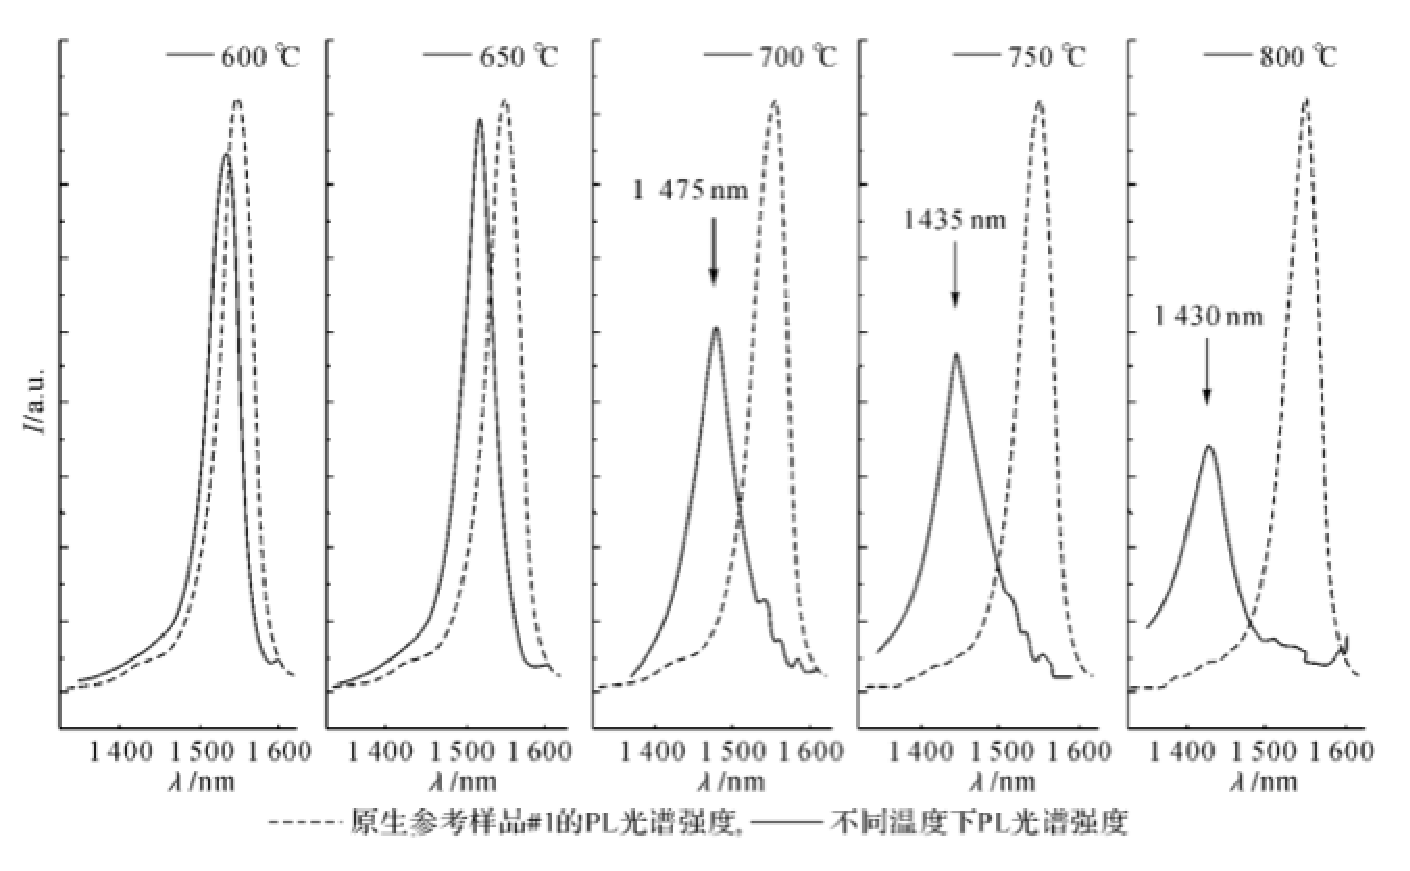
\includegraphics[width=1.0\textwidth]{./Pictures/icp.eps}\\
  \caption{在不同温度下退火2分钟之后的PL对比}
  \label{fig_icp}
\end{figure}

\begin{figure}[htbp]
  \centering
  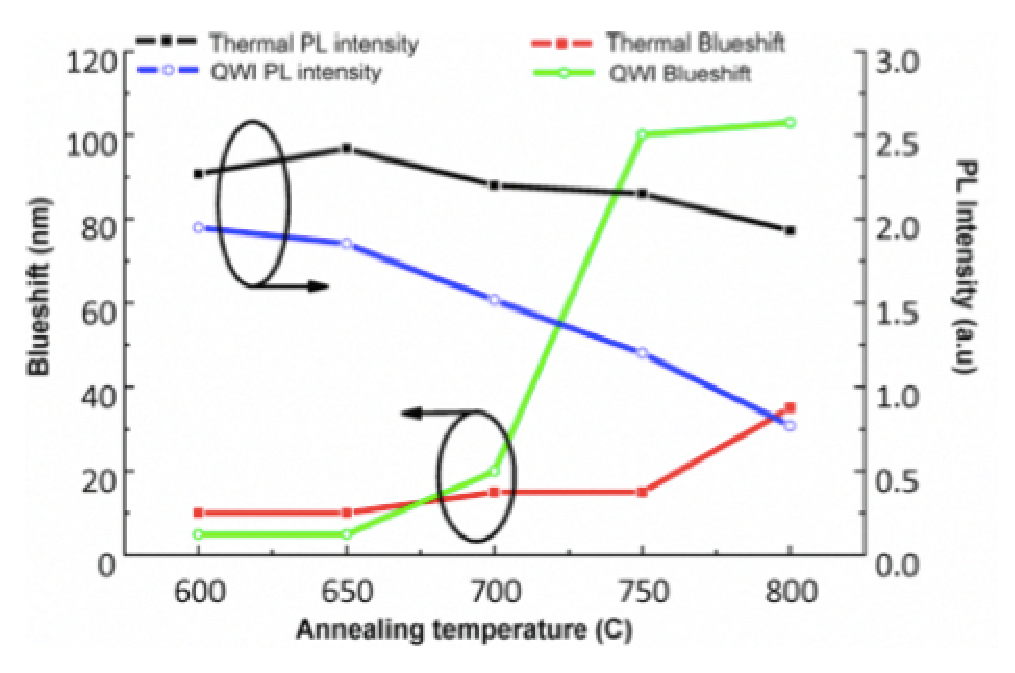
\includegraphics[width=0.5\textwidth]{./Pictures/icp2.eps}\\
  \caption{在不同退火温度条件下的PL蓝移和强度对比}
  \label{fig_icp2}
\end{figure}

\begin{figure}[htbp]
  \centering
  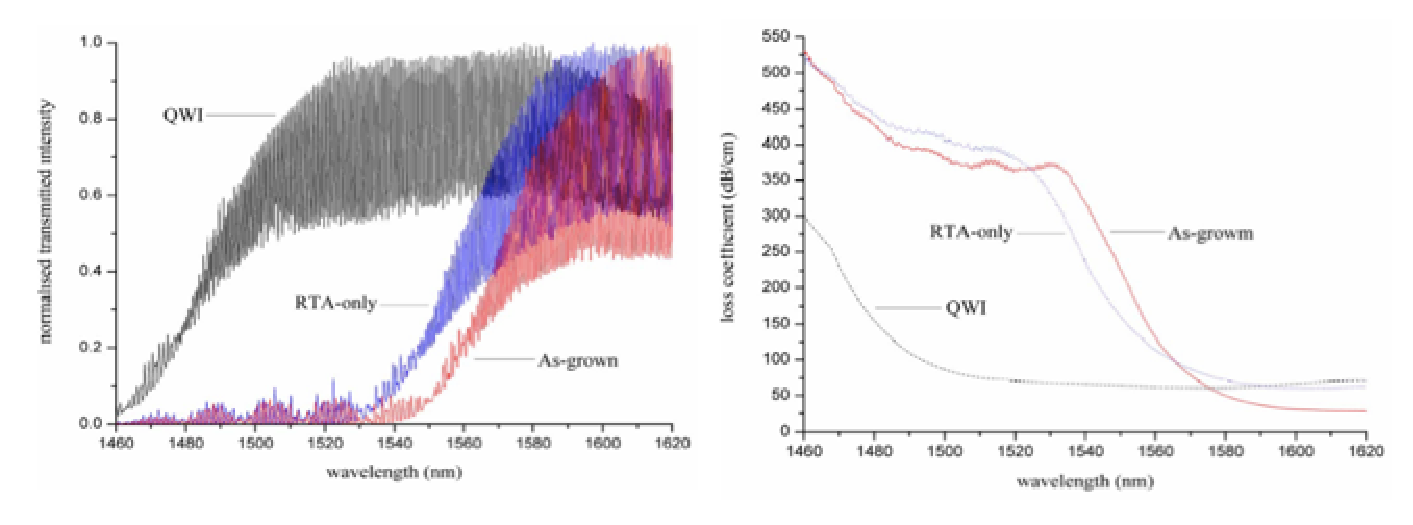
\includegraphics[width=1.0\textwidth]{./Pictures/icp3.eps}\\
  \caption{量子阱混杂、制作退火和原生材料制作的波导测试得到的透射谱(a)和计算得到的损耗(b)}
  \label{fig_icp3}
\end{figure}

%%%%%%%%%%%%%%%%%%%%
\subsection{溅射轰击方法}
%%%%%%%%%%%%%%%%%%%%

溅射轰击方法与等离子体轰击方法的原理有些相似。首先,芯片在溅射的过程中,在表面产生一层很薄的缺陷层。然后,这层缺陷在快速退火的条件下快速运动到量子阱区域,促进阱和垒的互相扩散,达到量子阱混杂的目的。这种方法也不需要购买额外的设备,因为溅射机是制作激光器电极的设备。如果需要对芯片做选择性的量子阱混杂,只需要在不做混杂的区域覆盖一层光刻胶或者二氧化硅掩膜,这些特点与等离子体轰击方法完全相同。不同的地方在于溅射的靶的材料。1998年,英国格拉斯哥大学的John~Marsh教授团队提出了利用溅射SiO$_2$和快速退火的方法实现量子阱混杂的效果\cite{Mcdougall1998Monolithic}。值得一提的是,如果SiO$_2$溅射在含有Ga原子的材料表面,就可能发生前面讨论的无杂质空位诱导的现象。所以在重复这个实验时,需要区分这两种现象,因为他们的原理是完全不同的。

2012年,浙江大学的Kaleem等人利用实验室设备,通过溅射SiO$_2$实现了量子阱混杂的目的。在2014年,浙江大学的朱洪力等提出了溅射氧化铝和氮化硅\cite{Zhu2014Bandgap}实现量子阱混杂的技术。在他们的实验中,经过溅射和快速热退火处理之后的InP量子阱片可以蓝移100~nm以上,如图~\ref{fig_sputter}。而混杂之后的波导损耗下降到了18~dB/cm,如图~\ref{fig_sputter2}~所示,这些都是比较理想的结果。

\begin{figure}[htbp]
  \centering
  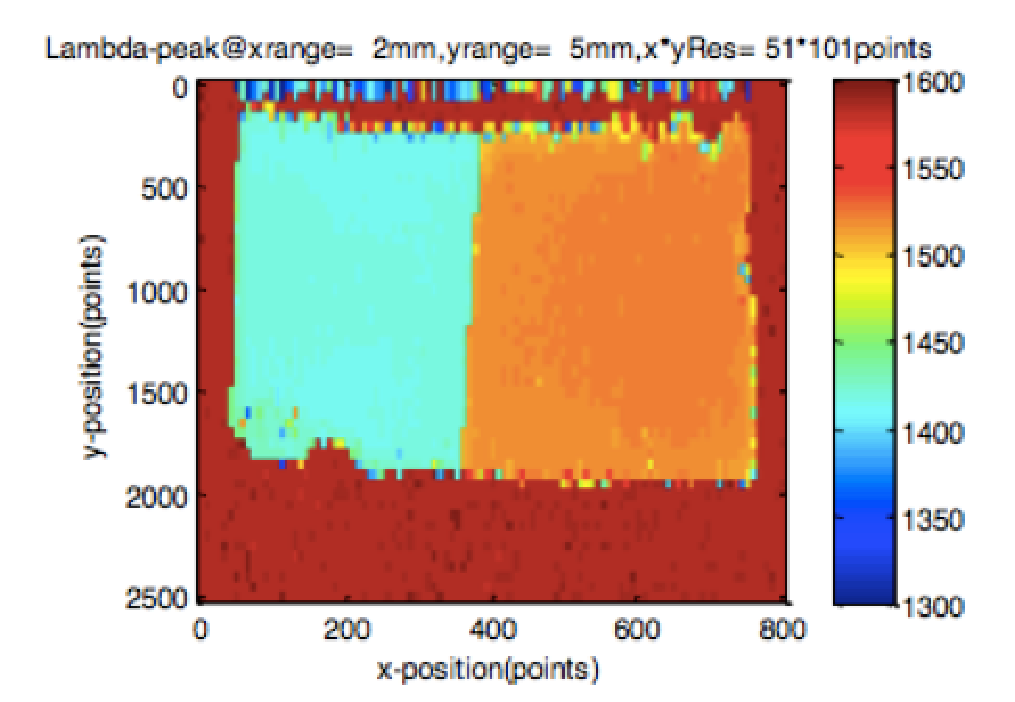
\includegraphics[width=0.7\textwidth]{./Pictures/sputter.eps}\\
  \caption{量子阱混杂前后的PL峰值波长对比}
  \label{fig_sputter}
\end{figure}

\begin{figure}[htbp]
  \centering
  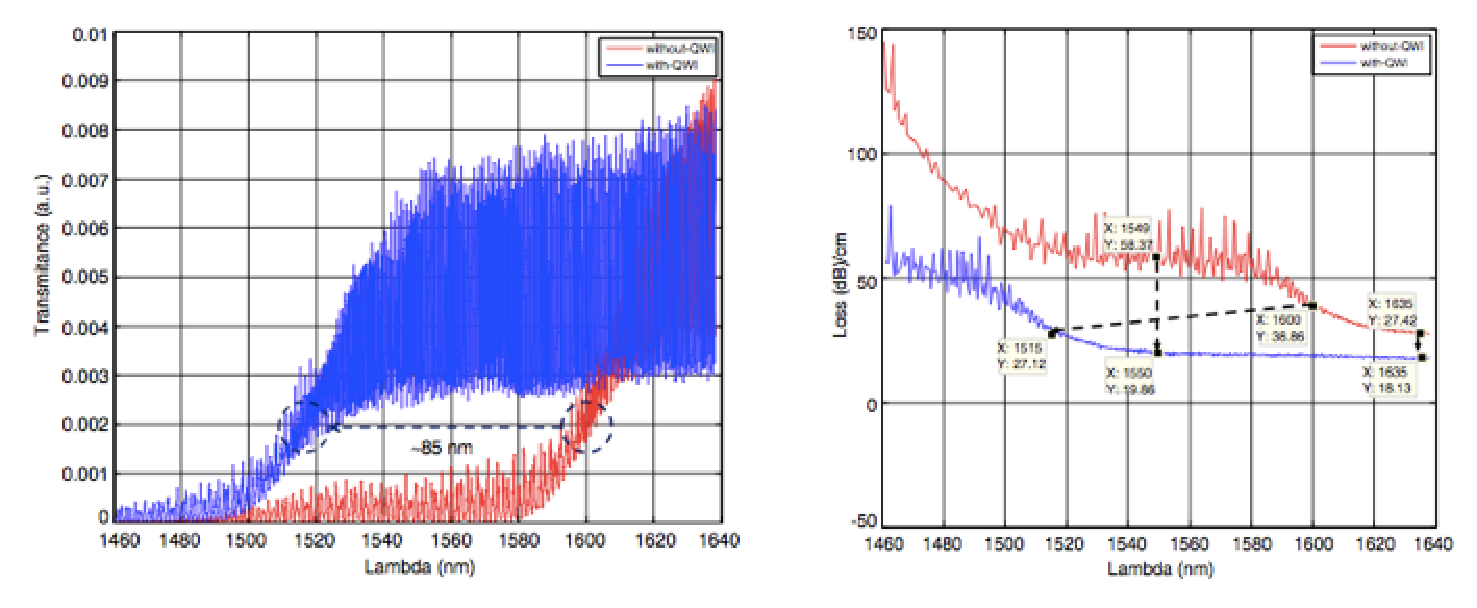
\includegraphics[width=1.0\textwidth]{./Pictures/sputter2.eps}\\
  \caption{量子阱混杂、制作退火和原生材料制作的波导测试得到的透射谱(a)和计算得到的损耗(b)}
  \label{fig_sputter2}
\end{figure}

%%%%%%%%%%%%%%%%%%%%
\subsection{离子注入方法}
%%%%%%%%%%%%%%%%%%%%

离子注入方法由离子注入和快速退火两个步骤组成。首先,特定种类的离子在非常高能量的离子注入机的加速下,直接打入芯片的内部。然后,在快速退火的作用下,这些离子促进了量子阱中的阱和垒的融合,最终达到改变禁带宽度的目的。

如图~\ref{fig_implantation}~所示,在D区域,磷离子在离子注入机的加速下直接注入到芯片的上包层,并在之后的快速退火的作用下,促进量子阱的阱和垒的互相融合。最有意思的是,在C、B、A区域,芯片表面生长了一层SiO$_2$掩膜。这层掩膜可以抵消一部分离子注入的能量,导致离子只能注入到稍浅的地方,最终这些区域的量子阱混杂程度会比没有掩膜的地方稍弱。通过制作不同厚度的SiO$_2$掩膜,就可以精确地控制量子阱混杂的程度,并且只需要一次快速退火就可以形成很多个不同禁带宽度的区域。

\begin{figure}[htbp]
  \centering
  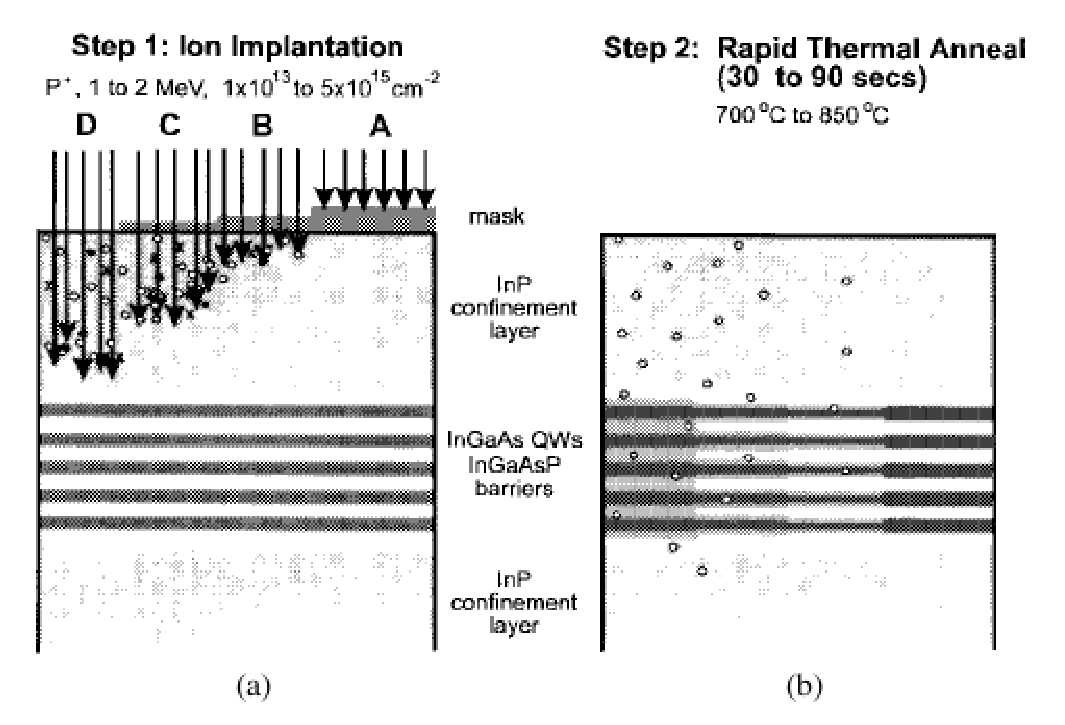
\includegraphics[width=0.7\textwidth]{./Pictures/implantation.eps}\\
  \caption{离子注入技术示意图}
  \label{fig_implantation}
\end{figure}

离子注入方法制作的无源波导的性能甚至比量子阱混杂之前的性能还要好\cite{He1995Bandgap}。如图~\ref{fig_implantation_wg_test}~所示,量子阱混杂之后,波导的禁带宽度相比于未混杂的波导,蓝移了90~nm左右。计算得到的损耗如图~\ref{fig_implantation_wg_loss}~所示。对于未混杂的波导,在透明传输的波长区域,比如1580~nm,波导的损耗大约是8cm$^{-1}$。对应到混杂之后的波导的1490~nm,波导的损耗只有5cm$^{-1}$左右。也就是说,经过离子注入方法制作的无源波导,损耗可以比未做处理之前还要低。

\begin{figure}[htbp]
  \centering
  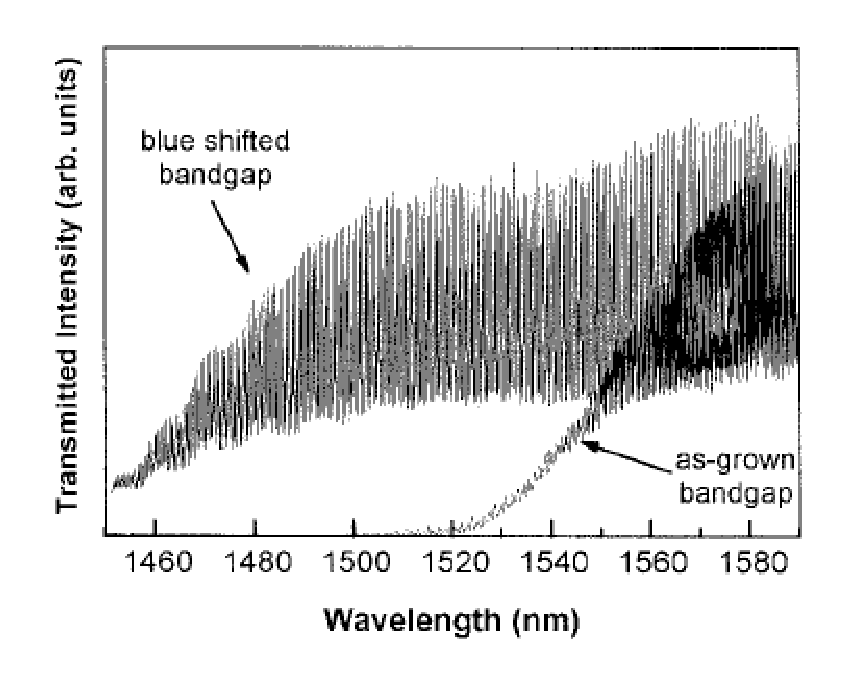
\includegraphics[width=0.5\textwidth]{./Pictures/implantation_wg_test.eps}\\
  \caption{测试得到的量子阱混杂和未混杂波导的透射光谱}
  \label{fig_implantation_wg_test}
\end{figure}

\begin{figure}[htbp]
  \centering
  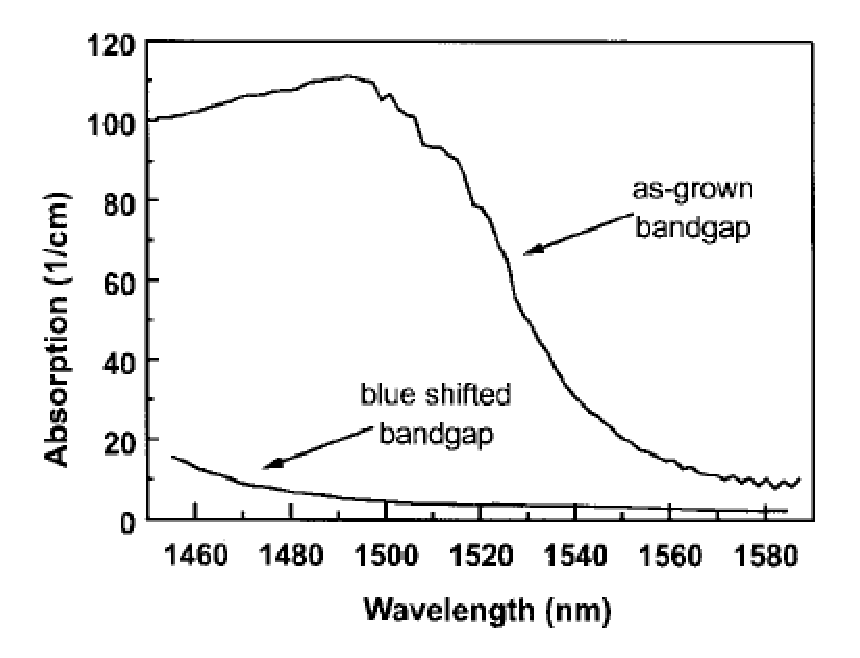
\includegraphics[width=0.5\textwidth]{./Pictures/implantation_wg_loss.eps}\\
  \caption{由透射光谱计算得到的损耗}
  \label{fig_implantation_wg_loss}
\end{figure}

利用离子注入技术制作的激光器的IV特性曲线如图~\ref{fig_implantation_laser}~所示。从图中可以看出,在量子阱混杂前后,两种激光器的IV曲线是非常相似的。在激光器工作的第一象限,两条曲线基本重合在一起。这说明,离子注入技术不会改变材料的电特性。

\begin{figure}[htbp]
  \centering
  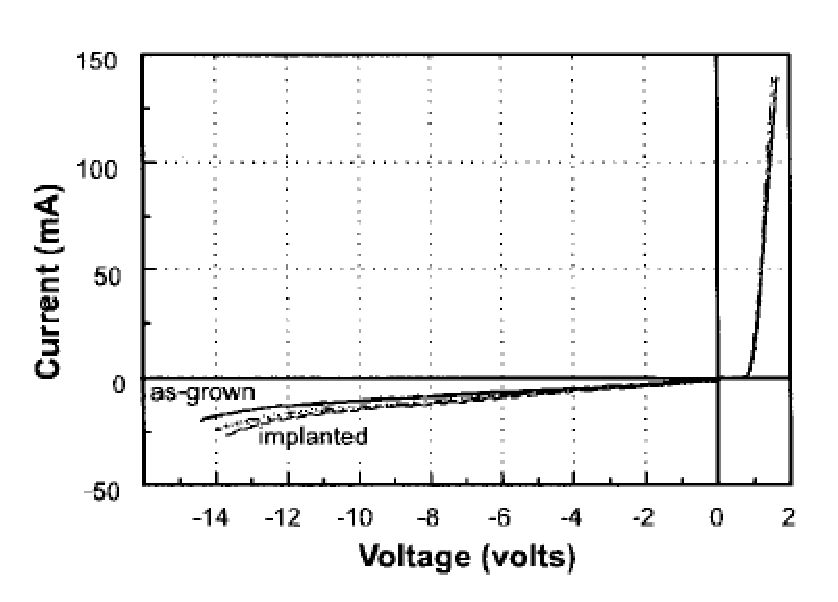
\includegraphics[width=0.5\textwidth]{./Pictures/implantation_laser.eps}\\
  \caption{由离子注入方法制作的激光器的IV特性曲线}
  \label{fig_implantation_laser}
\end{figure}

由于离子注入技术相对成熟,性能也很好,人们已经利用该技术制作了非常复杂的单片集成器件。第一章中介绍的Larry~Coldren教授制作的8$\times$8单片集成可调谐光路由器就是才采用了这个技术。

除了通常的高能离子注入方法之外,人们也尝试了高能聚焦离子注入机(FIB)实现量子阱混杂的方法。1998年,德国维尔兹堡大学的Johann~Peter~Reithmaier和Alfred~Forchel提出了利用高能聚焦离子注入机实现量子阱混杂的方法\cite{Reithmaier1998Focused}。原理上,他和普通的离子注入方法是完全一样的,所以他也有离子注入方法的大部分优势。不同的是他的处理面积很小,通常在纳米量级,这样可以用来制作增益耦合DFB激光器的光栅结构。当然由于离子束太小,当加工大范围的区域时,就显得太费时费力了。

%%%%%%%%%%%%%%%%%%%%
\subsection{各种量子阱混杂方法的比较}
%%%%%%%%%%%%%%%%%%%%

表~\ref{qwi_compare}~比较了本文中提到的各种量子阱混杂技术,仅供参考。
\begin{table}[htbp]
    \zihao{7}
    \caption{各种量子阱混杂方法的优缺点}
    \centering
    \label{qwi_compare}
    \begin{tabular}{ccccccccc}
        \hline
        \hline
                   &杂质诱导 &无杂质空位诱导 &低温生长InP &阳极氧化 &光吸收 &等离子体轰击 &溅射轰击 &离子注入\\
        \hline
        发表时间    &1981    &1986         &2000      &1998    &1997  &2002       &1998    &1995\\
        所需设备    &扩散炉或低能离子注入机 &PECVD &GSMBE &阳极氧化炉 &Nd:YAG激光器 &ICP &溅射机  &高能离子注入机\\
        GaAs可用    &是     &是     &否     &是     &否     &是     &是     &是\\
        InP可用     &是     &是     &是     &否     &是     &是     &是     &是\\
        无源波导损耗 &$\sim$10~dB/cm &$\sim$10~dB/cm &未知 &未知 &$\sim$10~dB/cm &$\sim$10~dB/cm &$\sim$10~dB/cm &$\sim$10~dB/cm\\
        电特性      &差     &好     &未知    &未知   &好     &好     &好     &好\\
        集成器件    &延长腔激光器 &延长腔激光器 &无 &无 &延长腔激光器 &延长腔激光器 &延长腔激光器 &延长腔激光器\\
        \hline
        \hline
    \end{tabular}
\end{table}


%%%%%%%%%%%%%%%%%%%%
\chapter{量子阱混杂技术的理论模拟}
%%%%%%%%%%%%%%%%%%%%

在量子阱混杂工艺研究不断取得进展的同时,人们也做了很多量子阱混杂的理论模拟方面的工作。这些模拟让人们更好地理解了量子阱混杂的机理,并指导人们在工艺上进一步优化。量子阱混杂的理论模拟最核心的问题是计算混杂之后的能带结构。也就是说,在原有的量子阱的基础上,通过加入混杂的工艺参数作为变量,计算得到混杂之后的能带结构。有了能带结构之后,就可以进一步计算材料的吸收系数,增益,折射率等等。最后,就可以计算出量子阱混杂对整个光器件的影响。这一章将详细介绍量子阱混杂的能带结构的计算方法。

%%%%%%%%%%%%%%%%%%%%
\section{薛定谔方程的数值解法}
%%%%%%%%%%%%%%%%%%%%

在半导体中,电子运动的状态可以通过解薛定谔方程得到。

\begin{equation}
    \label{schrodinger}
    \left[ -\frac{h^2}{ 2m^*} \bigtriangledown ^2 + V(r,t) \right] \psi(r,t) = ih \frac{\partial}{\partial t}  \psi(r,t) 
\end{equation}

其中,$m^*$是电子或者空穴的有效质量,$V(r,t)$是导带或者价带的势函数,$\bigtriangledown$是拉普拉斯算符,$\psi(r,t)$是与空间和时间有关的波函数。

然后,我们采用包络函数近似对上面的方程进行简化。在这个近似中,波函数的时间和空间分量可以分离开来,得到如下的函数式

\begin{equation}
    \label{schrodinger2}
    \left[ -\frac{h^2}{ 2m^*} \bigtriangledown ^2 + V(r) \right] \psi(r) = E  \psi(r) 
\end{equation}

其中$\psi(r)$是波函数的稳态解,E是能量特征值。接着,我们还需要用有效质量近似再对薛定谔方程做一次简化,并且写成一维方向上的函数式,最后可以写成

\begin{equation}
    \label{eq_effective_mass}
    \left[ -\frac{\hbar^2}{2} \frac{d}{dx} \frac{1}{m^*(x)} + V(x) \right] \psi(x) = E \psi(x)
\end{equation}

我们只需要知道有效质量$m^*(x)$和势能$V(x)$在每个x上的值,就可以求出整个系统的特征值和特征函数,对应半导体能级的能量$E$和波函数$\psi(x)$。求解上述方程的数值方法有很多,包括有限差分法、传输矩阵法和有限元法等等。我们选择了相对简单,并且精度足够用的传输矩阵法。首先,我们需要将上面方程中的势函数和有效质量进行离散化,如图~\ref{fig_tmm}~所示。在每一小段的离散区间内,势函数和有效质量被视为不变,也就是说,在$x_j\le x<x_j+\Delta_j=x_{j+1}$时,$V_j=V(x_j)$,$m^*_j=m^*(x_j)$,而在这一段的末尾进行$V_j\to V_{j+1}$,$m^*_j\to m^*_{j+1}$的跳变。在$x_j\le x<x_{j+1}$的区间内,方程~\ref{eq_effective_mass}~的解可以表示为

\begin{equation}
    \label{eq_effective_mass_solution}
    \psi(x) = A_j \exp [i k_j (x-x_j)] + B_j \exp [-i k_j (x-x_j)]
\end{equation}

\begin{figure}[htbp]
  \centering
  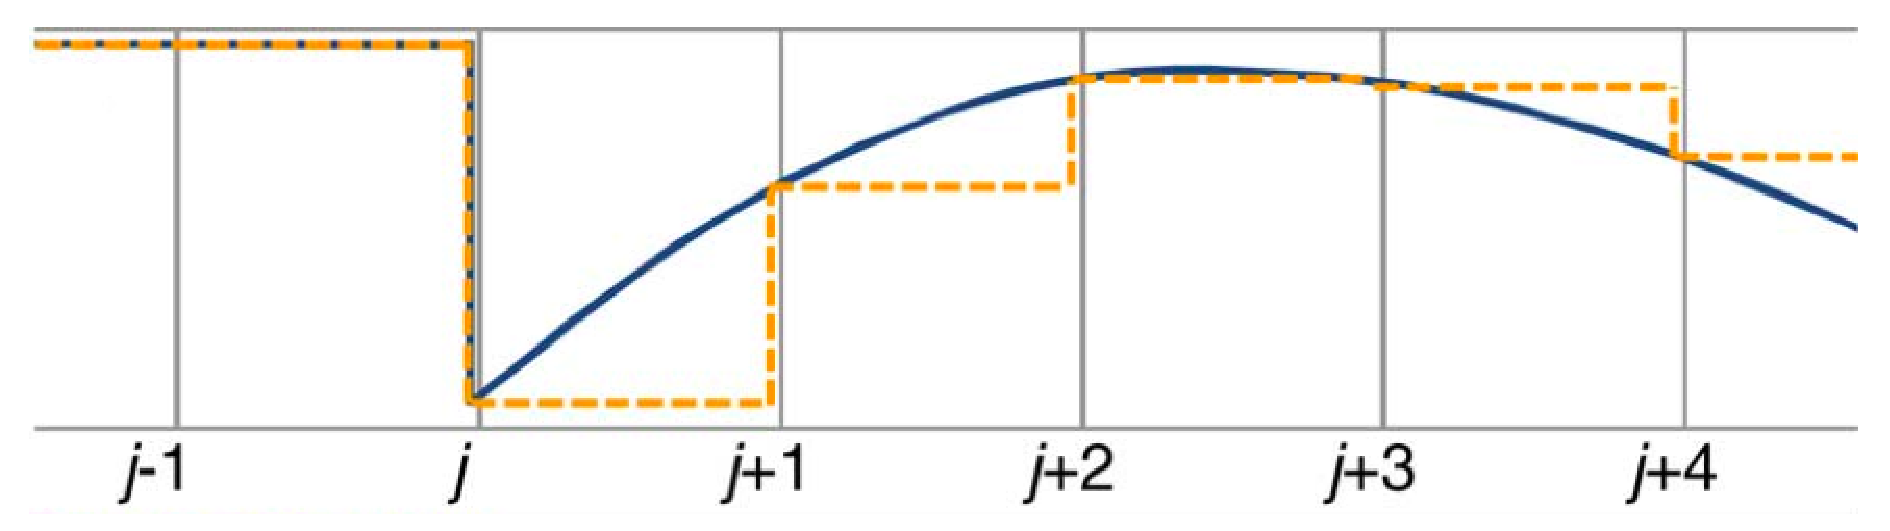
\includegraphics[width=0.7\textwidth]{./Pictures/tmm.eps}\\
  \caption{传输矩阵法对势函数和有效质量的离散化,实线代表精确值,虚线代表离散值\cite{Jirauschek2009Accuracy}}
  \label{fig_tmm}
\end{figure}

其中$k_j=\sqrt{2 m^*_j (E-V_j)} / \hbar$是波函数的波数。同时,方程~\ref{eq_effective_mass}~的边界条件需要满足波函数和它的导数在每个区间的连接点上连续,即如下两个方程

\begin{equation}
    \label{eq_boundary_1}
    \psi_{j-1}(x_{j-1}) = \psi_j(x_{j-1}) 
\end{equation}

\begin{equation}
    \label{eq_boundary_2}
    \frac{1}{m^*_{j-1}} \frac{d}{dx} [ \psi_{j-1}(x_{j-1}) ] = \frac{1}{m^*_j} \frac{d}{dx} [\psi_j(x_{j-1})]
\end{equation}

将边界条件方程~\ref{eq_boundary_1}~和~\ref{eq_boundary_2}~代入方程~\ref{eq_effective_mass},就可以得到相邻两层的波函数振幅之间的关系,即

\begin{equation}
    \label{eq_tmm}
    \begin{pmatrix} A_{j+1} \\ B_{j+1} \end{pmatrix} = T_{j,j+1} \begin{pmatrix} A_{j} \\ B_{j} \end{pmatrix}
\end{equation}

其中的传输矩阵为

\begin{equation}
    \label{eq_transfer_matrix}
    T_{j,j+1} = \frac{1}{2\beta_{j+1}} \begin{pmatrix} \beta_{j+1}+\beta_j & \beta_{j+1}-\beta_j  \\ \beta_{j+1}-\beta_j  & \beta_{j+1}+\beta_j  \end{pmatrix} \begin{pmatrix} e^{ik_j\Delta_j} & 0 \\ 0 & e^{-ik_j\Delta_j} \end{pmatrix}
\end{equation}

其中$\beta_j = k_j/m^*_j$。最后,我们可以将每一层的传输矩阵从左往右连续相乘,得到如下的方程

\begin{equation}
    \label{eq_tmm_serial}
    \begin{pmatrix} A_{N} \\ B_{N} \end{pmatrix} = T_{N-1,N}T_{N-2,N-1}\cdots T_{0,1} \begin{pmatrix} A_{0} \\ B_{0} \end{pmatrix} =  \begin{pmatrix} T_{11} & T_{12} \\ T_{21} & T_{22} \end{pmatrix} \begin{pmatrix} A_{0} \\ B_{0} \end{pmatrix}
\end{equation}

其中$N$是分段的总段数。这个连续的方程需要满足收敛条件,也就是$A_0=B_N=0$,对应于最后的方程

\begin{equation}
    \label{eq_t22}
    T_{22}=0
\end{equation}

上面的方程是一个关于E的复数方程,它的所有解,从小到大依次就是每一个能级,代入到前面的波动方程~\ref{eq_effective_mass_solution}~中,就可以得到每个x点上的波函数。

为了验证程序的正确性,我们选择了文献中的AlGaAs-GaAs量子阱结构\cite{jonsson1990solving},其势能和有效质量如表~\ref{tmm_sample}~所示。由于导带和价带的能级计算方法完全一样,这里只给出导带的计算结果,如表所示。我们将文献中的传输矩阵法\cite{jonsson1990solving}、有限元法\cite{nakamura1989finite}的结果和我们的结果作比较,发现结果基本上是一致的,误差最大仅有0.03\%,说明了该程序是正确的。存在的一些微小偏差主要来源于对x轴的取值不同。x轴的离散化的步长和整个x轴的长度,会对能级的结果产生细微的影响。此外,我们还计算了前四个能级对应的波函数振幅的平方,并且与势函数叠加在一起,如图~\ref{fig_waves}~所示。结果再一次验证了程序的正确性。

\begin{table}[htbp]
    \zihao{5}
    \caption{用于传输矩阵法计算的AlGaAs-GaAs量子阱的导带参数}
    \centering
    \label{tmm_sample}
    \begin{tabular}{cccc}
        \hline
        阱宽(nm) & 阱深(meV) & 阱内有效质量(m0) & 阱外有效质量(m0)\\
        \hline
        20                & 225                 & 0.067                          & 0.0919\\
        \hline
    \end{tabular}
\end{table}

\begin{table}[htbp]
    \zihao{5}
    \caption{计算得到的导带的前四个能级(meV)}
    \centering
    \label{tmm_sample_result}
    \begin{tabular}{cccc}
        \hline
        能级 & 传输矩阵法\cite{jonsson1990solving} & 有限元法\cite{nakamura1989finite} & 我们的程序(相对于有限元法的误差) \\
        \hline
        1       & 9.966              & 9.967            & 9.970(0.03\%) \\
        2       & 39.77              & 39.77            & 39.78(0.03\%) \\
        3       & 88.92              & 88.93            & 88.96(0.03\%) \\
        4       & 155.59            & 155.61          & 155.64(0.01\%) \\
        \hline
    \end{tabular}
\end{table}

\begin{figure}[htbp]
  \centering
  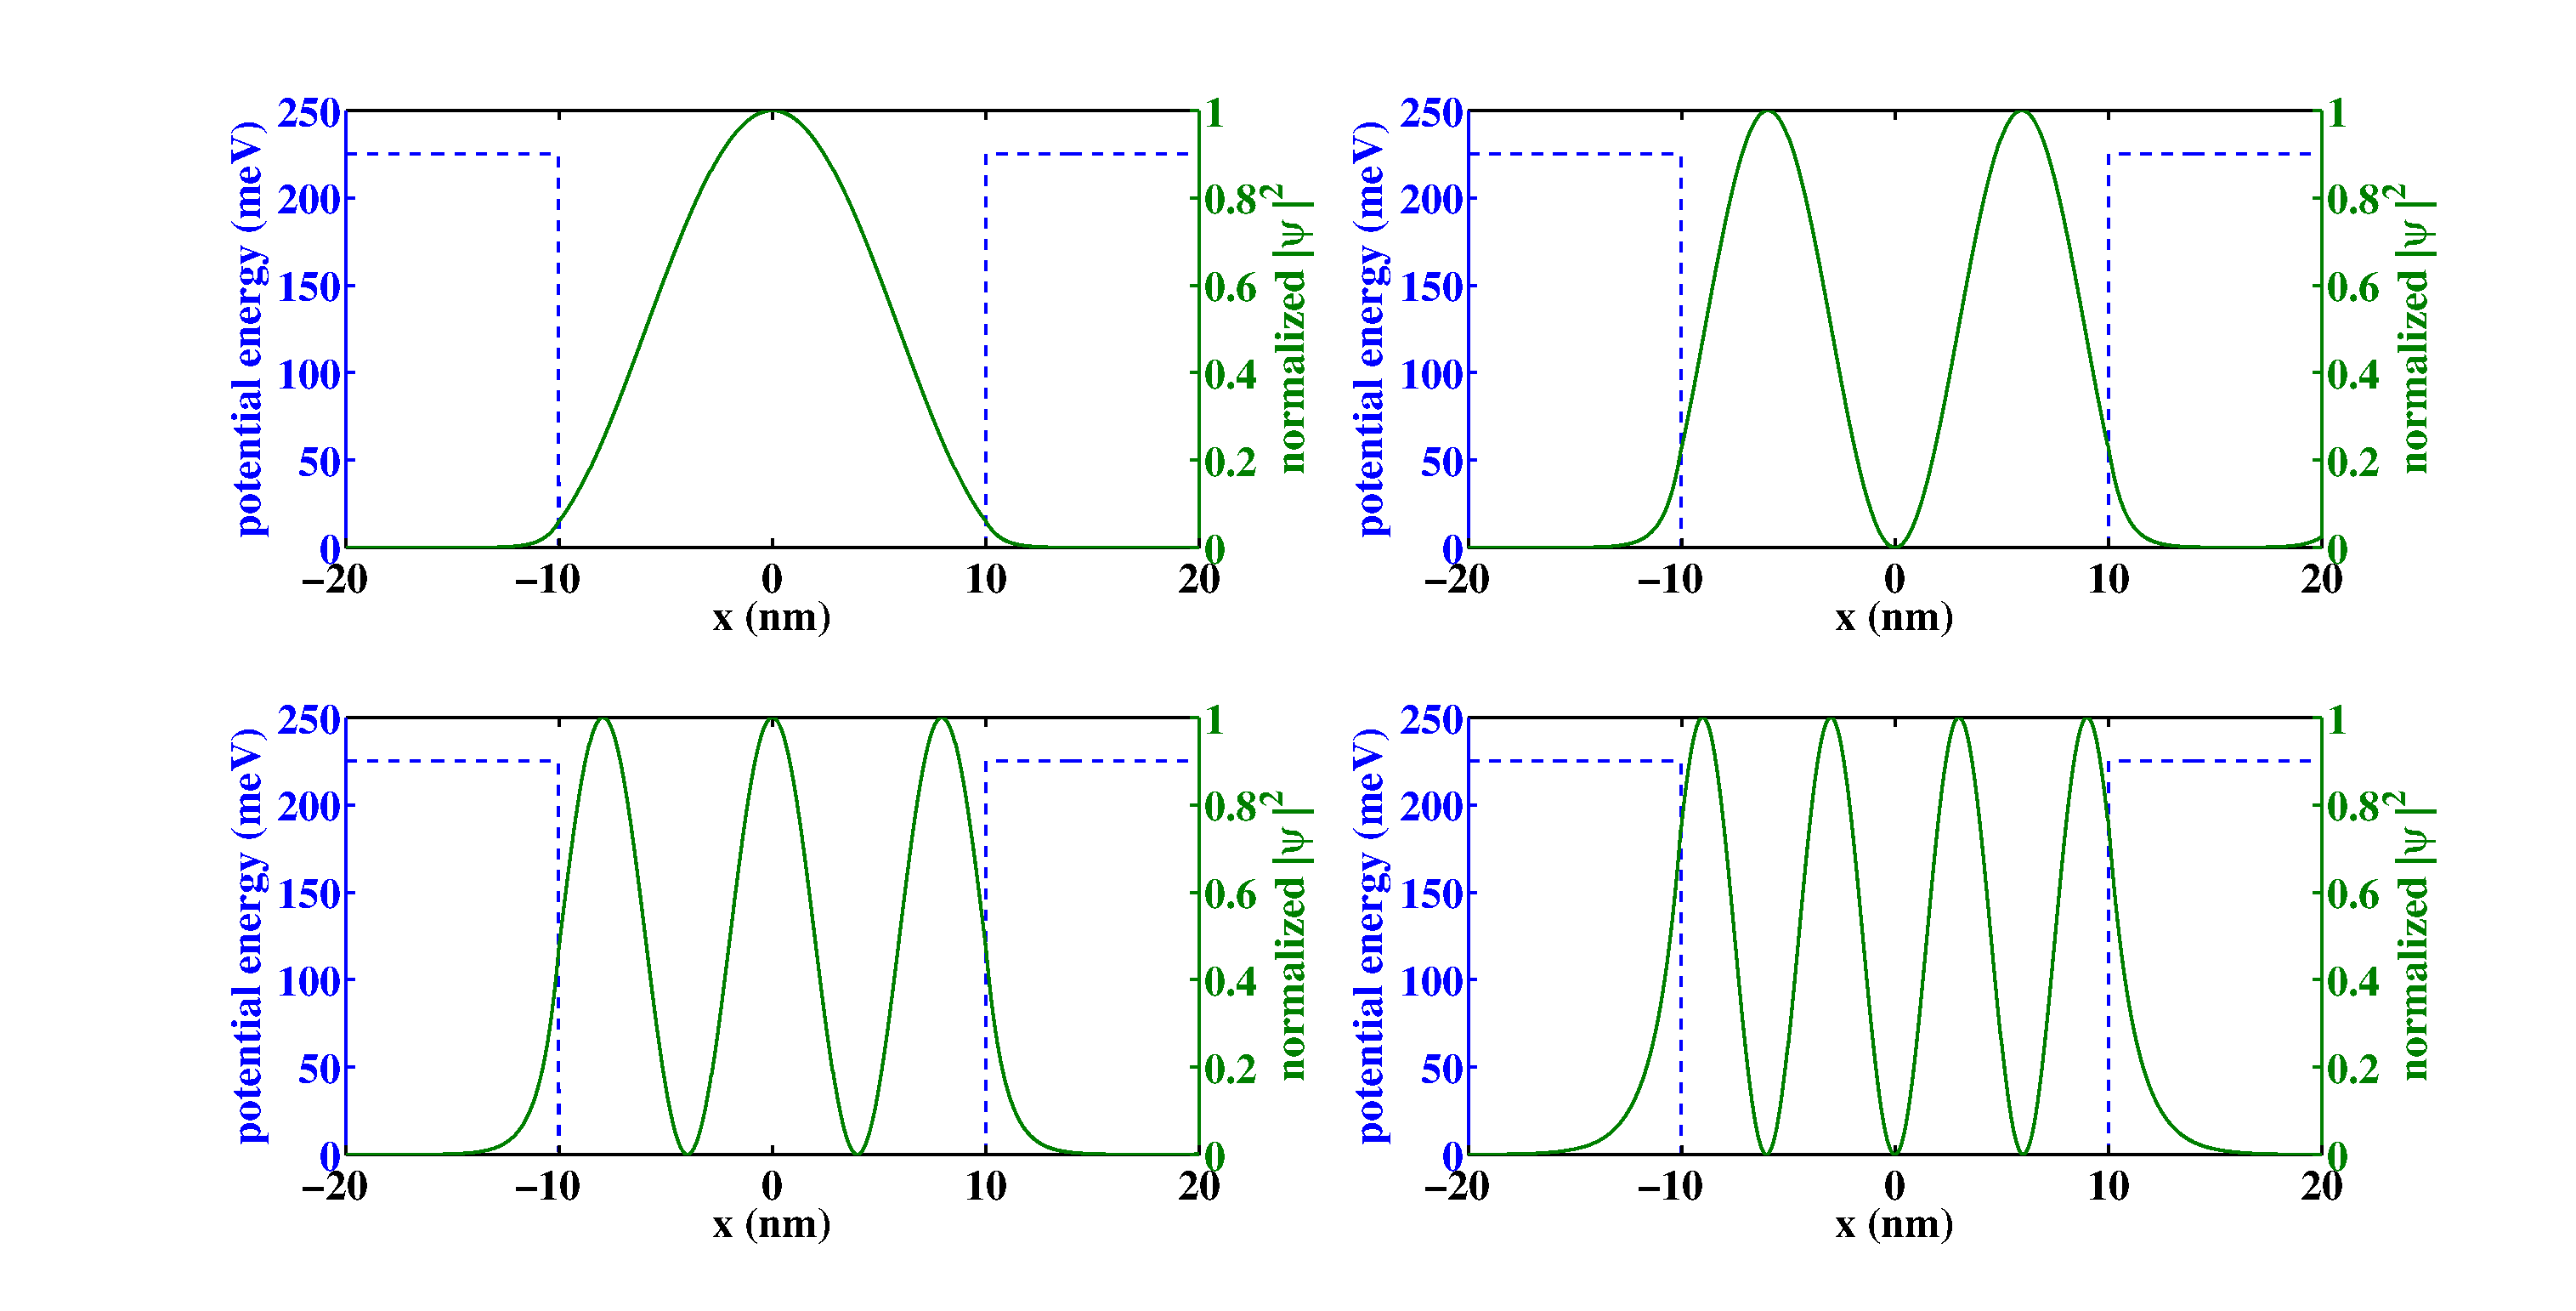
\includegraphics[width=1.0\textwidth]{./Pictures/waves.eps}\\
  \caption{势函数以及前四个能级波函数振幅的平方}
  \label{fig_waves}
\end{figure}

%%%%%%%%%%%%%%%%%%%%
\section{III-V量子阱的能带结构}
%%%%%%%%%%%%%%%%%%%%

\begin{figure}[htbp]
  \centering
  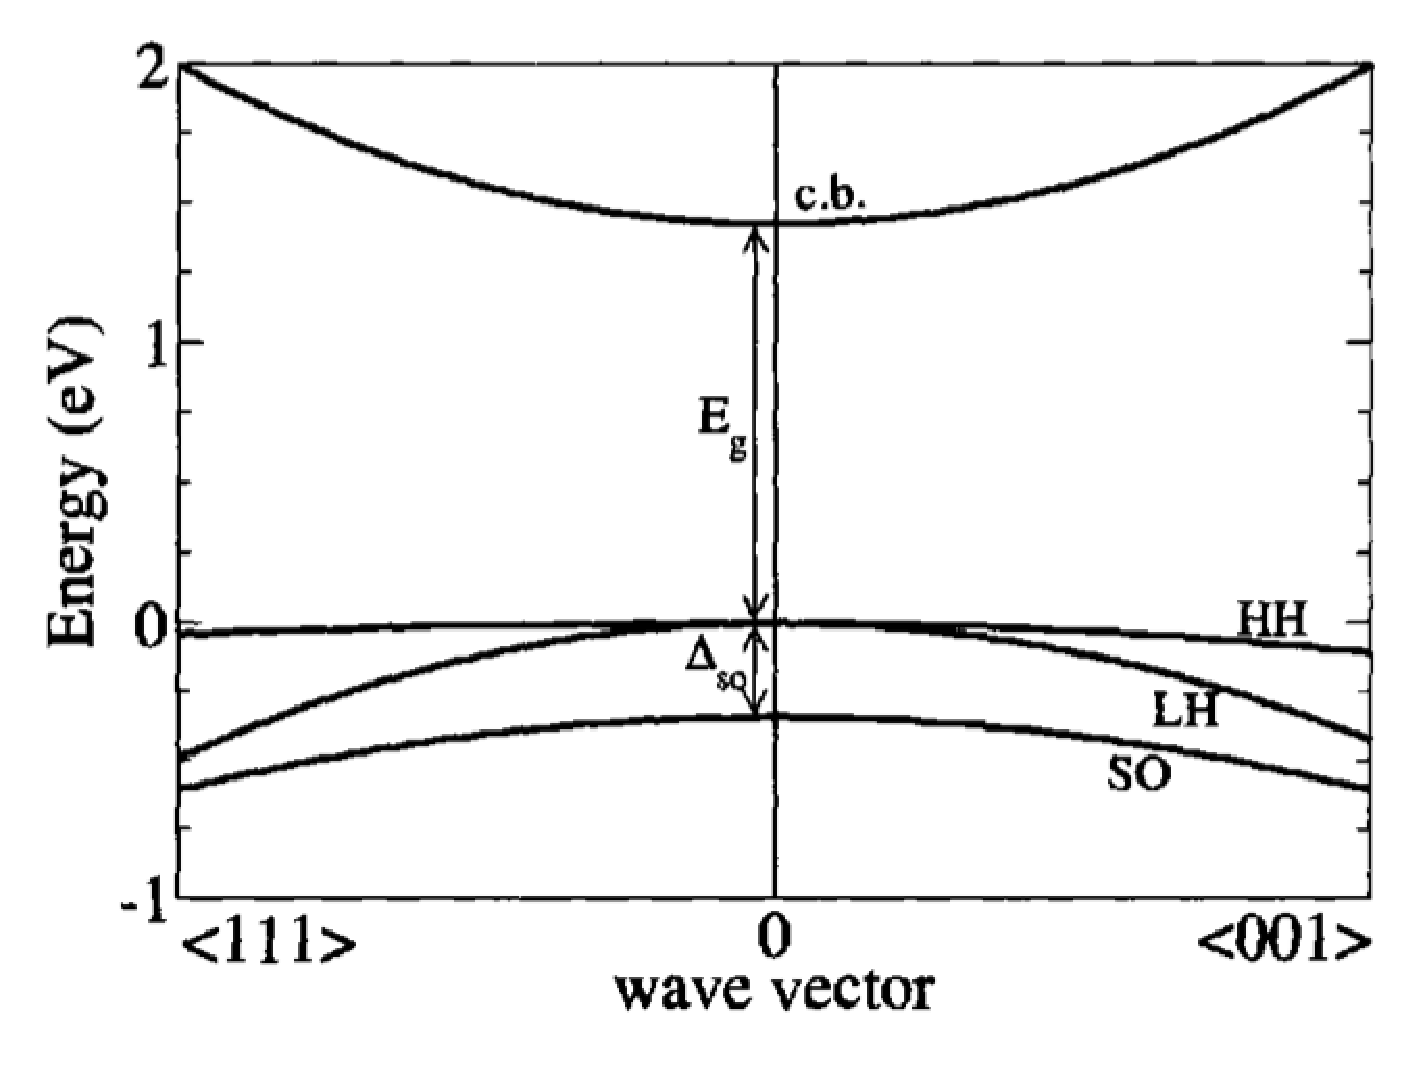
\includegraphics[width=0.5\textwidth]{./Pictures/bands.eps}\\
  \caption{III-V半导体在布里渊区的$\Gamma$点附近的导带和价带示意图\cite{Harrison2009Quantum}}
  \label{fig_bands}
\end{figure}

对于III-V量子阱材料来说,价带的能带结构比导带要复杂一些,如图~\ref{fig_bands}。通常,在布里渊区的中心附近,存在两个重叠的价带,以及在不远处的第三条能带。前面两条能带分别叫做重空穴(HH)和轻空穴(LH)带。随着波矢向远离$\Gamma$点方向运动时,重空穴带比轻空穴带向下弯曲的更慢一些,也就是对应了更大的有效质量,所以它被成为重空穴带。第三条能带叫做自旋分裂(SO)能带。也就是说,III-V材料通常包含三条价带和一条导带。为了计算这些能带,最常用也是最简单的方法是采用$k\cdot p$微扰理论,推导出计算这些能带的哈密顿算子。1955年,Luttinger和Kohn得到了关于三个价带的$6\times6$哈密顿算子,以及其中两个价带(HH和LH)的$4\times4$哈密顿算子\cite{Luttinger1955Motion}。1966年Pidgeon和Brown提出了包含导带的$8\times8$哈密顿算子\cite{Pidgeon1966Interband}~。这里,我们给出Luttinger和Kohn的$6\times6$哈密顿算子如下:

\begin{equation}
    \label{eq_6times6}
    H = \left[\begin{array}{cccccc}P+Q & 0 & -S & R & (1/\sqrt{2})S & \sqrt{2}R \\0 & P+Q & -R\dag & -S^\dag & -\sqrt{2}R^\dag & (1/\sqrt{2})S^\dag \\-S^\dag & -R & P-Q & 0 & \sqrt{2}Q & \sqrt{3/2}S \\R^\dag & -S & 0 & P-Q & \sqrt{3/2}S^\dag & \sqrt{2}Q \\(1/\sqrt{2})S^\dag & -\sqrt{2}R & \sqrt{2}Q & \sqrt{3/2}S & P+\Delta_{SO} & 0 \\\sqrt{2}R^\dag & (1/\sqrt{2})S & \sqrt{3/2}S\dag & \sqrt{2}Q & 0 & P+\Delta_{SO}\end{array}\right]
\end{equation}
其中

\begin{equation}
    P = \left( \frac{h^2}{2m_0} \right) \gamma_1 (k^2_x + k^2_y + k^2_z)
\end{equation}
\begin{equation}
    Q = \left( \frac{h^2}{2m_0} \right) \gamma_2 (k^2_x + k^2_y - 2k^2_z)
\end{equation}
\begin{equation}
    R = \left( \frac{h^2}{2m_0} \right) \sqrt{3} [-\gamma_2 (k^2_x - k^2_y) + 2i \gamma_3 k_x k_y]
\end{equation}
\begin{equation}
    S = \left( \frac{h^2}{2m_0} \right) 2 \sqrt{3} \gamma_3 k_z (k_x - ik_y)
\end{equation}
其中$\gamma_{1,2,3}$是Luttinger参数,$\Delta_{SO}$是自旋轨道分裂能量。其中的参数很容易在各种书籍或文章中查到,这里不再赘述。根据以上方程,我们就可以计算出三条价带关于波失的关系。这里考虑一种特殊情况,在布里渊区的中心,我们可以将上面的算子进一步简化,即$k_x=k_y=k_z=0$时,算子变成了

\begin{equation}
    H(k=0) = \left[\begin{array}{cccccc}0 & 0 & 0 & 0 & 0 & 0 \\0 & 0 & 0 & 0 & 0 & 0 \\0 & 0 & 0 & 0 & 0 & 0 \\0 & 0 & 0 & 0 & 0 & 0 \\0 & 0 & 0 & 0 & \Delta_{SO} & 0 \\0 & 0 & 0 & 0 & 0 & \Delta_{SO}\end{array}\right]
\end{equation}
上面矩阵的含义是,当k=0时,导带和价带的能量E=0,并且自旋轨道分裂能量与他们的能力差为$\Delta_{SO}$。当我们计算量子阱时,正需要考虑这种情况。

此外,我们还需要考虑应变对价带的影响。应变在III-V半导体中表现为6个分量:$\epsilon_{xx}$,$\epsilon_{yy}$,$\epsilon_{zz}$,$\epsilon_{xy}$,$\epsilon_{zx}$和$\epsilon_{yz}$。他们对$6\times6$哈密顿算子的影响如下面的方程所示\cite{Calvin1992Spin}:

\begin{equation}
    P \rightarrow P + P_{\epsilon} ,  P_{\epsilon} = - a_v (\epsilon_{xx} + \epsilon_{yy} + \epsilon_{zz})
\end{equation}
\begin{equation}
    Q \rightarrow Q + Q_{\epsilon} ,  Q_{\epsilon} = - \frac{b}{2} (\epsilon_{xx} + \epsilon_{yy} -2 \epsilon_{zz})
\end{equation}
\begin{equation}
    R \rightarrow R + R_{\epsilon} ,  R_{\epsilon} = \frac{\sqrt{3}}{2} b (\epsilon_{xx} - \epsilon_{yy}) - i d \epsilon_{xy})
\end{equation}
\begin{equation}
    S \rightarrow S + S_{\epsilon} ,  S_{\epsilon} = - d (\epsilon_{zx} -i \epsilon_{yz})
\end{equation}
其中$a_v$,$b$,$d$是各个方向上的形变势能系数。在实际的应变量子阱材料中,随着材料在z方向外延的过程中发生了应变,所以各个方向的分量可以表示为

\begin{equation}
    \epsilon_{xy} = \epsilon_{yz} = \epsilon_{zx} = 0
\end{equation}
\begin{equation}
    \epsilon_{xx} = \epsilon_{yy} = \frac{a_0 - a_{latt}}{a_{latt}} / a_{latt}
\end{equation}
\begin{equation}
    \epsilon_{zz} = - \frac{2 C_{12}}{C_{11}}  \epsilon_{xx}
\end{equation}
其中$C_{11}$和$C_{12}$是弹性刚度系数,$a_0$是基底的晶格常数(通常都是晶格匹配的)。此时,我们再回过头来看$6\times6$哈密顿算子在k=0时的情况,他已经变成

\begin{equation}
    H = \left[\begin{array}{cccccc}P_{\epsilon}+Q_{\epsilon} & 0 & 0 & 0 & 0 & 0 \\0 & P_{\epsilon}+Q_{\epsilon} & 0 & 0 & 0 & 0 \\0 & 0 & P_{\epsilon}-Q_{\epsilon} & 0 & \sqrt{2}Q_{\epsilon} & 0 \\0 & 0 & 0 & P_{\epsilon}-Q_{\epsilon} & 0 & \sqrt{2}Q_{\epsilon} \\0 & 0 & \sqrt{2}Q_{\epsilon} & 0 & Q_{\epsilon}+\Delta_{SO} & 0 \\0 & 0 & 0 & \sqrt{2}Q_{\epsilon} & 0 & \Delta_{SO}\end{array}\right]
\end{equation}
这个方程比没有应变的情况要复杂的多。经过计算,我们可以得到k=0时三个价带在布里渊区中心的能量分别为

\begin{equation}
    E_{HH}(0) = P_{\epsilon} + Q_{\epsilon}
\end{equation}
\begin{equation}
    E_{LH}(0) = P_{\epsilon} - \frac{1}{2} \left( Q_{\epsilon} - \Delta_{SO} + \sqrt{\Delta^2_{SO} + 2 \Delta^2_{SO} Q_{\epsilon} + 9 Q^2_{\epsilon}} \right)
\end{equation}
\begin{equation}
    E_{SO}(0) = P_{\epsilon} - \frac{1}{2} \left( Q_{\epsilon} - \Delta_{SO} - \sqrt{\Delta^2_{SO} + 2 \Delta^2_{SO} Q_{\epsilon} + 9 Q^2_{\epsilon}} \right)
\end{equation}

最后,我们考虑导带和价带的偏置比,就可以得打导带和价带的势能函数方程

\begin{equation}
    \label{V_c}
    V_c(z) = Q_c E_g(z) - (1-Q_c)S_\perp(z)
\end{equation}
\begin{equation}
    \label{V_HH}
    V_{HH}(z) = (1-Q_c)[E_g(z) - S_\perp(z)] + S_\parallel(z)
\end{equation}
\begin{eqnarray}
    \label{V_LH}
    V_{LH}(z)&=& (1-Q_c)[E_g(z) - S_\perp(z)] \notag\\
    && +0.5[S_\parallel(z) + \Delta_0(z)] \notag\\
    && -0.5 \sqrt{9S_\parallel^2(z)-2S_\parallel^2(z)\Delta_0(z)+\Delta_0^2(z)}
\end{eqnarray}
其中
\begin{equation}
    \label{S_perp}
    S_\perp(z) = -2a_v(z)[1-\frac{C_{12}(z)}{C_{11}(z)}] \epsilon(z)
\end{equation}
\begin{equation}\label{S_parallel}
    S_\parallel(z) = -b(z)[1+\frac{2C_{12}(z)}{C_{11}(z)}] \epsilon(z)
\end{equation}
\begin{equation}\label{a_v}
    a_v(z) = -\frac{1}{3}[C_{11}(z)+2C_{12}(z)] \frac{dE_g}{dp}(z)
\end{equation}
\begin{equation}\label{epsilon}
    \epsilon(z) = \frac{a_{InP}(z)-a(z)}{a(z)}
\end{equation}
方程中的参数已经在表~\ref{parametertable}~中给出。如无特别说明,本章中采用的量子阱均采用表~\ref{RedShiftSample}~中的结构。


\begin{table}[!htb]
    \zihao{6}
    \caption{室温条件下(300K)InGaAsP量子阱材料的参数}
    \centering
    \label{parametertable}
    \begin{tabular}{llll}
        \hline
        \hline
        符号 & 参数 & $In_{x}Ga_{1-x}As_{y}P_{1-y}$ & 单位\\
        \hline
        $Q_c:Q_v$ & 能带偏移分裂比 & $0.6:0.4$ & $-$\\
        $E_g(z)$ & 禁带宽度 & $1.35-1.17y+0.668(1-x)-0.069y(1-x)+0.18y^2$ & eV\\
                                  && $+0.03(1-x)y^2+0.758(1-x)^2-0.322y(1-x)^2$ &\\
        $\Delta_0(z)$ & 自旋轨道分裂 & $0.34(1-x)y+0.43xy+0.10(1-x)(1-y)+0.10x(1-y)$ & eV\\
        $m_e$ & 电子质量 & $0.91095\times10{-30}$ & kg\\
        $m_c^*(z)$ & 电子有效质量 & $0.0632(1-x)y+0.0213xy+0.17(1-x)(1-y)+0.077x(1-y)$ & $m_e$\\
        $m_{\perp HH}^*(z)$ & 垂直方向 & $0.5(1-x)y+0.41xy+0.54(1-x)(1-y)+0.12x(1-y)$ & $m_e$\\
                            & 重空穴有效质量 &&\\
        $m_{\perp LH}^*(z)$ & 垂直方向& $0.088(1-x)y+0.024xy+0.16(1-x)(1-y)+0.12x(1-y)$ & $m_e$\\
                            & 轻空穴有效质量&&\\
        $m_{\parallel HH}^*(z)$ & 水平方向 & $0.11(1-x)y+0.031xy+0.19(1-x)(1-y)+0.15x(1-y)$ & $m_e$\\
                                & 重空穴有效质量 &&\\
        $m_{\parallel LH}^*(z)$ & 水平方向 & $0.23(1-x)y+0.082xy+0.34(1-x)(1-y)+0.29x(1-y)$ & $m_e$\\
                                & 轻空穴有效质量 &&\\
        $a(z)$ & 晶格常数 & $0.56533(1-x)y+0.60584xy+0.54512(1-x)(1-y)+0.58688x(1-y)$ & nm\\
        $C_{11}(z)$ & 弹性刚度常数 & $11.8(1-x)y+8.329xy+14.12(1-x)(1-y)+10.22x(1-y)$ & $10^{11}dyn/cm^2$\\
        $C_{12}(z)$ & 弹性刚度常数 & $5.38(1-x)y+4.526xy+6.253(1-x)(1-y)+5.76x(1-y)$ & $10^{11}dyn/cm^2$\\
        $dE_g/dP(z)$ & 水静压系数 & $11.5(1-x)y+10.0xy+11.0(1-x)(1-y)+8.5x(1-y)$ & $10^{-6}eV/bar$\\
        $b(z)$ & 剪切形变势能 & $-1.7(1-x)y-1.8xy-1.5(1-x)(1-y)-2.0x(1-y)$ & eV\\
        \hline
        \hline
    \end{tabular}
\end{table}


\begin{table}[htbp]
    \zihao{5}
    \caption{The layer structure for the undoped InGaAsP/InP single quantum well}
    \centering
    \label{RedShiftSample}
    \begin{tabular}{cccc}
        \hline
        \hline
        No. & Composition & Thickness(nm) & Layer\\
        \hline
        5 & $In_{0.53}Ga_{0.47}As$ & 500 & Buffer/cap\\
        4 & InP & 500 & Barrier/cap\\
        3 & $In_{0.71}Ga_{0.29}As_{0.61}P_{0.39}$ & 3.5 & Well\\
        2 & InP & 300 & Barrier\\
        1 & InP & $-$ & substrate\\
        \hline
        \hline
    \end{tabular}
\end{table}

%%%%%%%%%%%%%%%%%%%%
\section{扩散模型}
%%%%%%%%%%%%%%%%%%%%

量子阱混杂的过程是一个原子扩散的过程。为了模拟这个过程,我们需要一个数学模型用来表示材料组分和扩散程度之间的关系。在这里,我们采用$A_{x}B_{1-x}C_{y}D_{1-y}$这样的标记来表示III-V族半导体化合物,其中A和B代表第III族的原子,C和D代表第V族原子,x和y分别代表相应元素的摩尔比。量子阱混杂之后,第III族和第V族的原子摩尔比可以表示为两个与晶体生长方向($z$方向)相关的函数,即$w(z)$和$v(z)$。

半导体中的扩散过程可以用沿着晶体生长方向的菲克第二定律来表示,即

\begin{equation}
  \frac{\partial{C}}{\partial{t}}=D\frac{\partial^2{C}}{\partial{z^2}}
\end{equation}

其中$C$表示材料组分,$D$表示扩散系数。一般来说,扩散系数在整个量子阱中被视为常量。在这里,我们需要引入一个用来表示扩散程度的系数,即扩散长度$L_d$。扩散长度的定义为$L_d=\sqrt{Dt}$,其中$D$是扩散系数,$t$是加热过程的时间。假设一个$In_{wx}Ga_{1-wx}As_{wy}P_{1-wy}/In_{bx}Ga_{1-bx}As_{by}P_{1-by}$的单量子阱结构,量子阱混杂之后In和As的的组分函数可以分别表示为

\begin{eqnarray}
    w(z)&=&wx-\frac{bx-wx}{2} \times \biggr[2-\textrm{erf}\biggr(\frac{L_z+2z}{4L_d^{III}}\biggr) -\textrm{erf}\biggr(\frac{L_z-2z}{4L_d^{III}}\biggr)\biggr]
\end{eqnarray}

\begin{eqnarray}
    v(z)&=&wy-\frac{by-wy}{2} \times \biggr[2-\textrm{erf}\biggr(\frac{L_z+2z}{4L_d^{V}}\biggr) -\textrm{erf}\biggr(\frac{L_z-2z}{4L_d^{V}}\biggr)\biggr]
\end{eqnarray}

在这种情况下,扩散可以同时在第III族和第V族的元素中进行,分别对应了$L_d^{III}$和$L_d^V$两个扩散长度。他们的比值$k=L_d^V/L_d^{III}$是一个影响量子阱混杂效果的重要因素。同理,对于$Al_{wx}Ga_{1-wx}As/Al_{bx}Ga_{1-bx}As$量子阱来说,由于不存在第V族元素的扩散,k值永远等于0。

\begin{figure}[htbp]
    \centering
    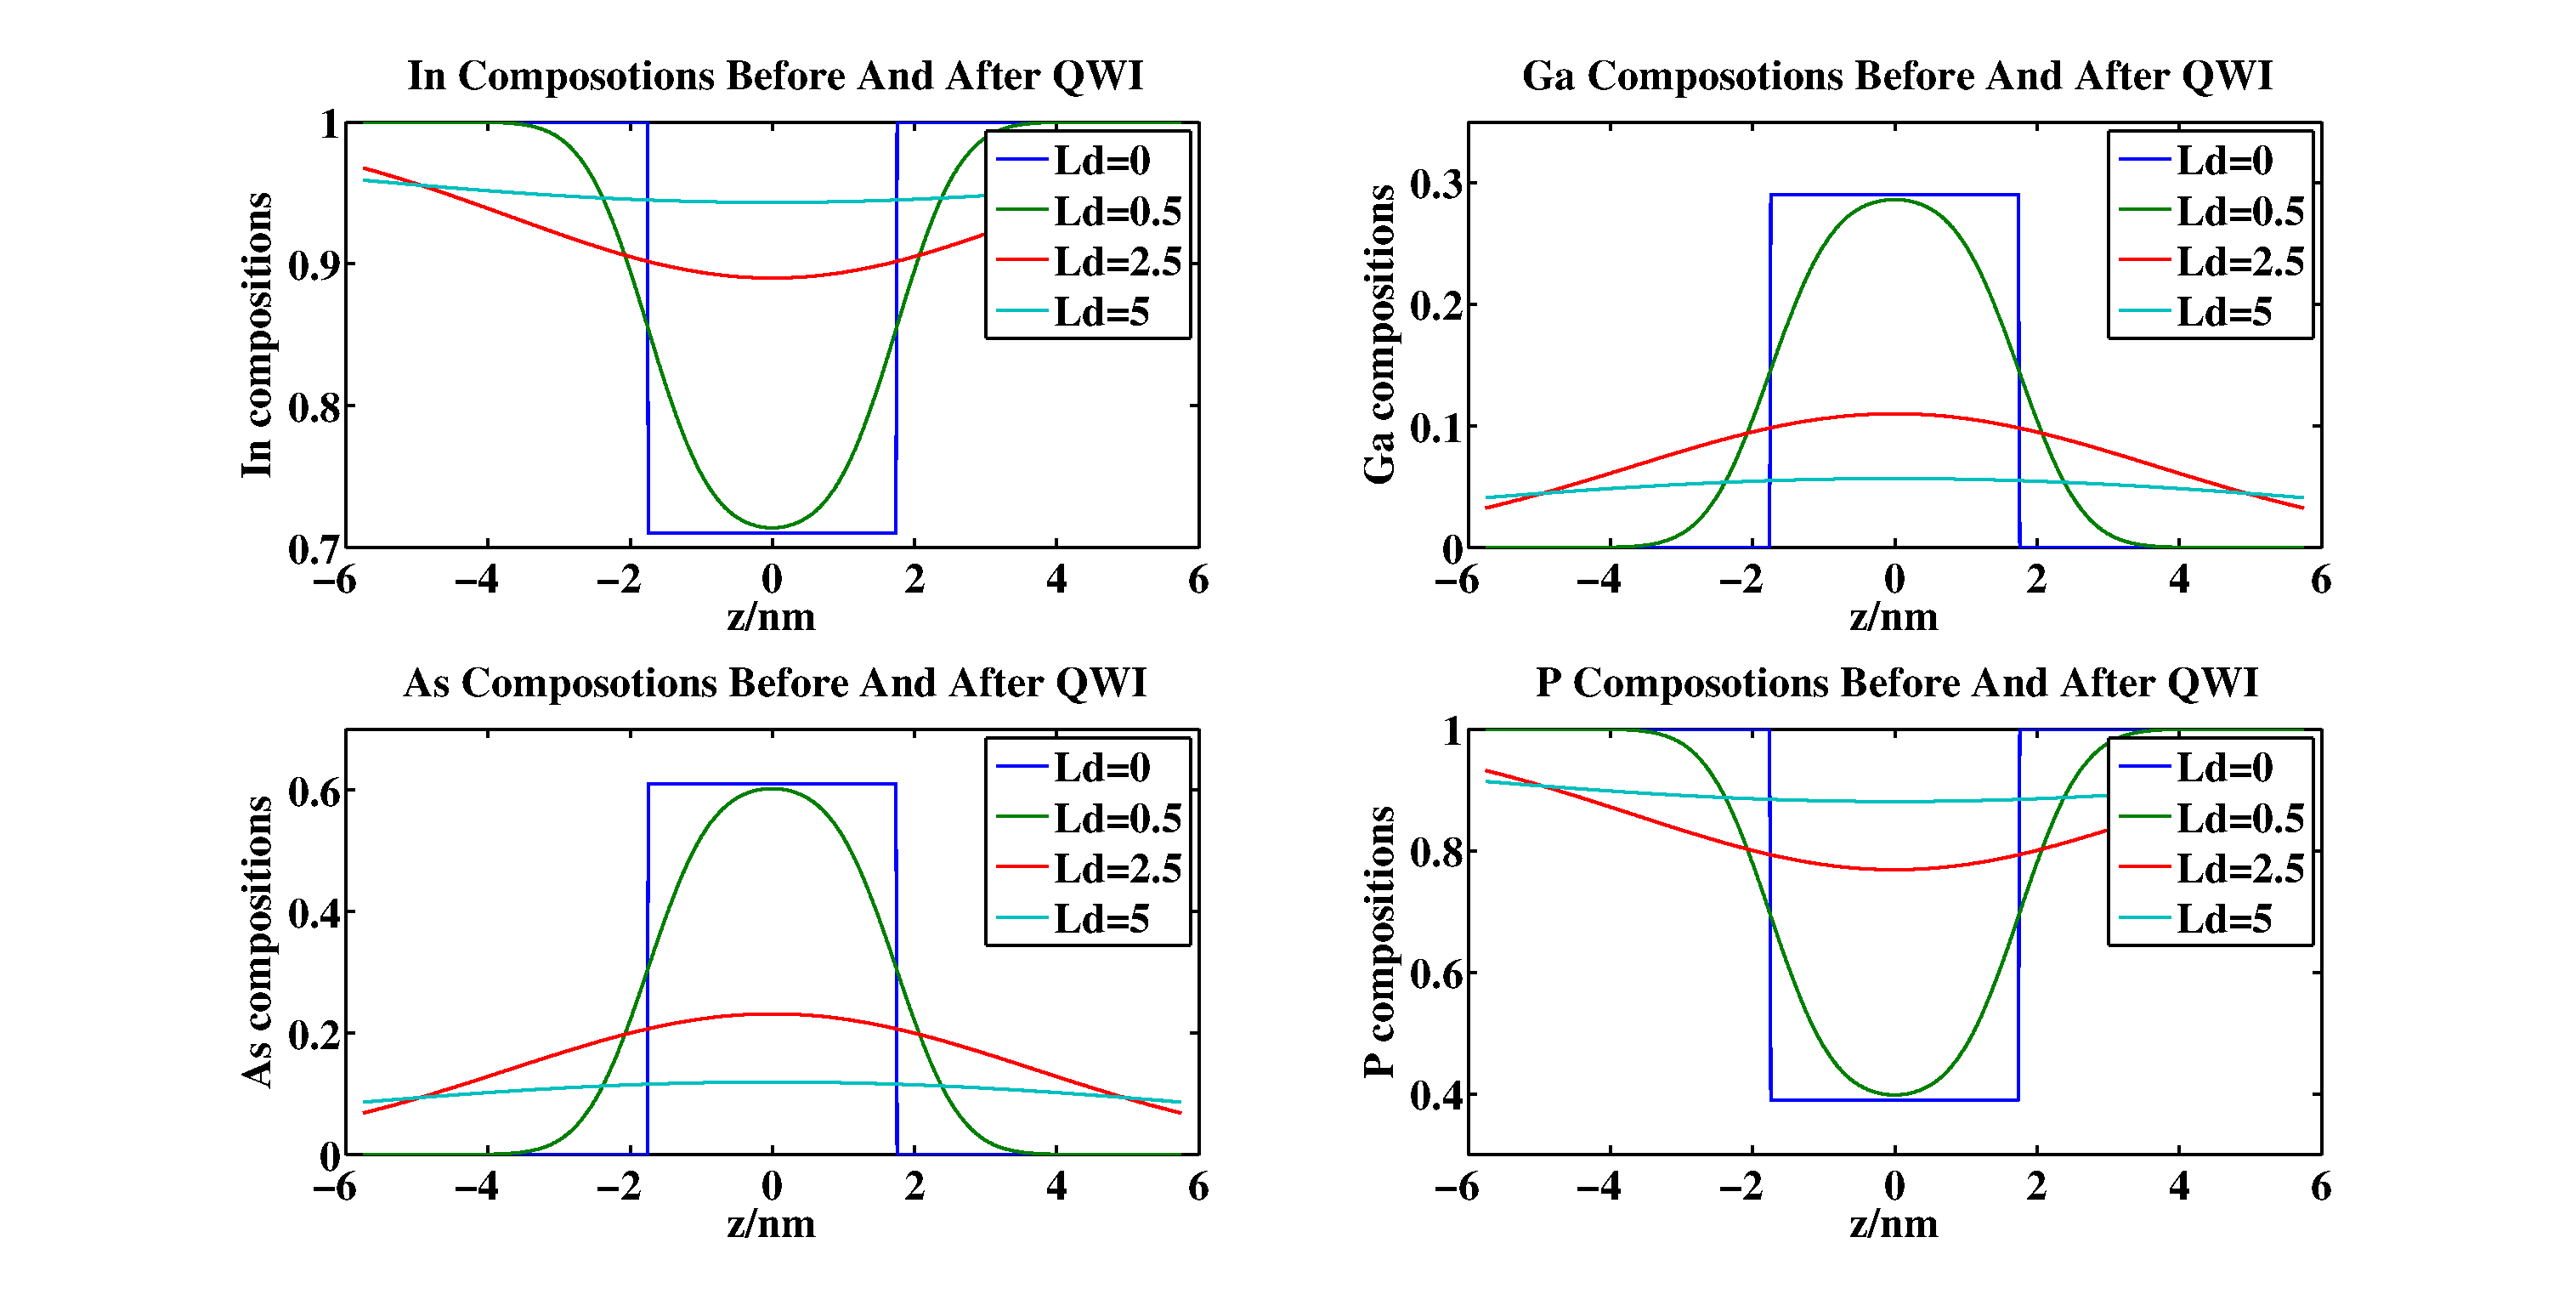
\includegraphics[width=1.0\textwidth]{./Pictures/composition.eps}
    \caption{In、Ga、As、P元素在不同的扩散长度条件下的组分分布}
    \label{fig_composition}
\end{figure}

图~\ref{fig_composition}~表示In、Ga、As、P元素在不同的扩散长度条件下的组分分布。当扩散长度为0时,量子阱不发生扩散,也就是不发生混杂的元素组分分布。当扩散长度为0.5nm时,元素组分仅在阱的中间位置与扩散之前的相同。当扩散长度为2.5nm时,整个阱的组分都已经发生很大变化。当扩散长度为5nm时,阱和垒的组分基本没有区别,呈现一条水平线。

%%%%%%%%%%%%%%%%%%%%
\section{扩散长度对能带结构的影响}
%%%%%%%%%%%%%%%%%%%%

为了讨论扩散长度对量子阱混杂的影响,我们假设扩散的k值始终等于1,这样就排除了k值的干扰,而且III族和V族的元素具有相同的扩散长度。我们选择了扩散长度从0到1nm,间隔0.1~nm的11种情况,分别计算了导带和两条价带的最低能级的能量,如图~\ref{fig_Ld_1}~所示。左边的图表示In的组分变化,其实也可以看成体材料的势函数沿着材料生长方向的分布。显然,随着扩散长度的增加,量子阱的势函数的底部在不断往上抬升,这导致了导带、重空穴带和轻空穴带能级的上升,这一点从右边的图就可以清楚的看出来。

\begin{figure}[htbp]
    \centering
    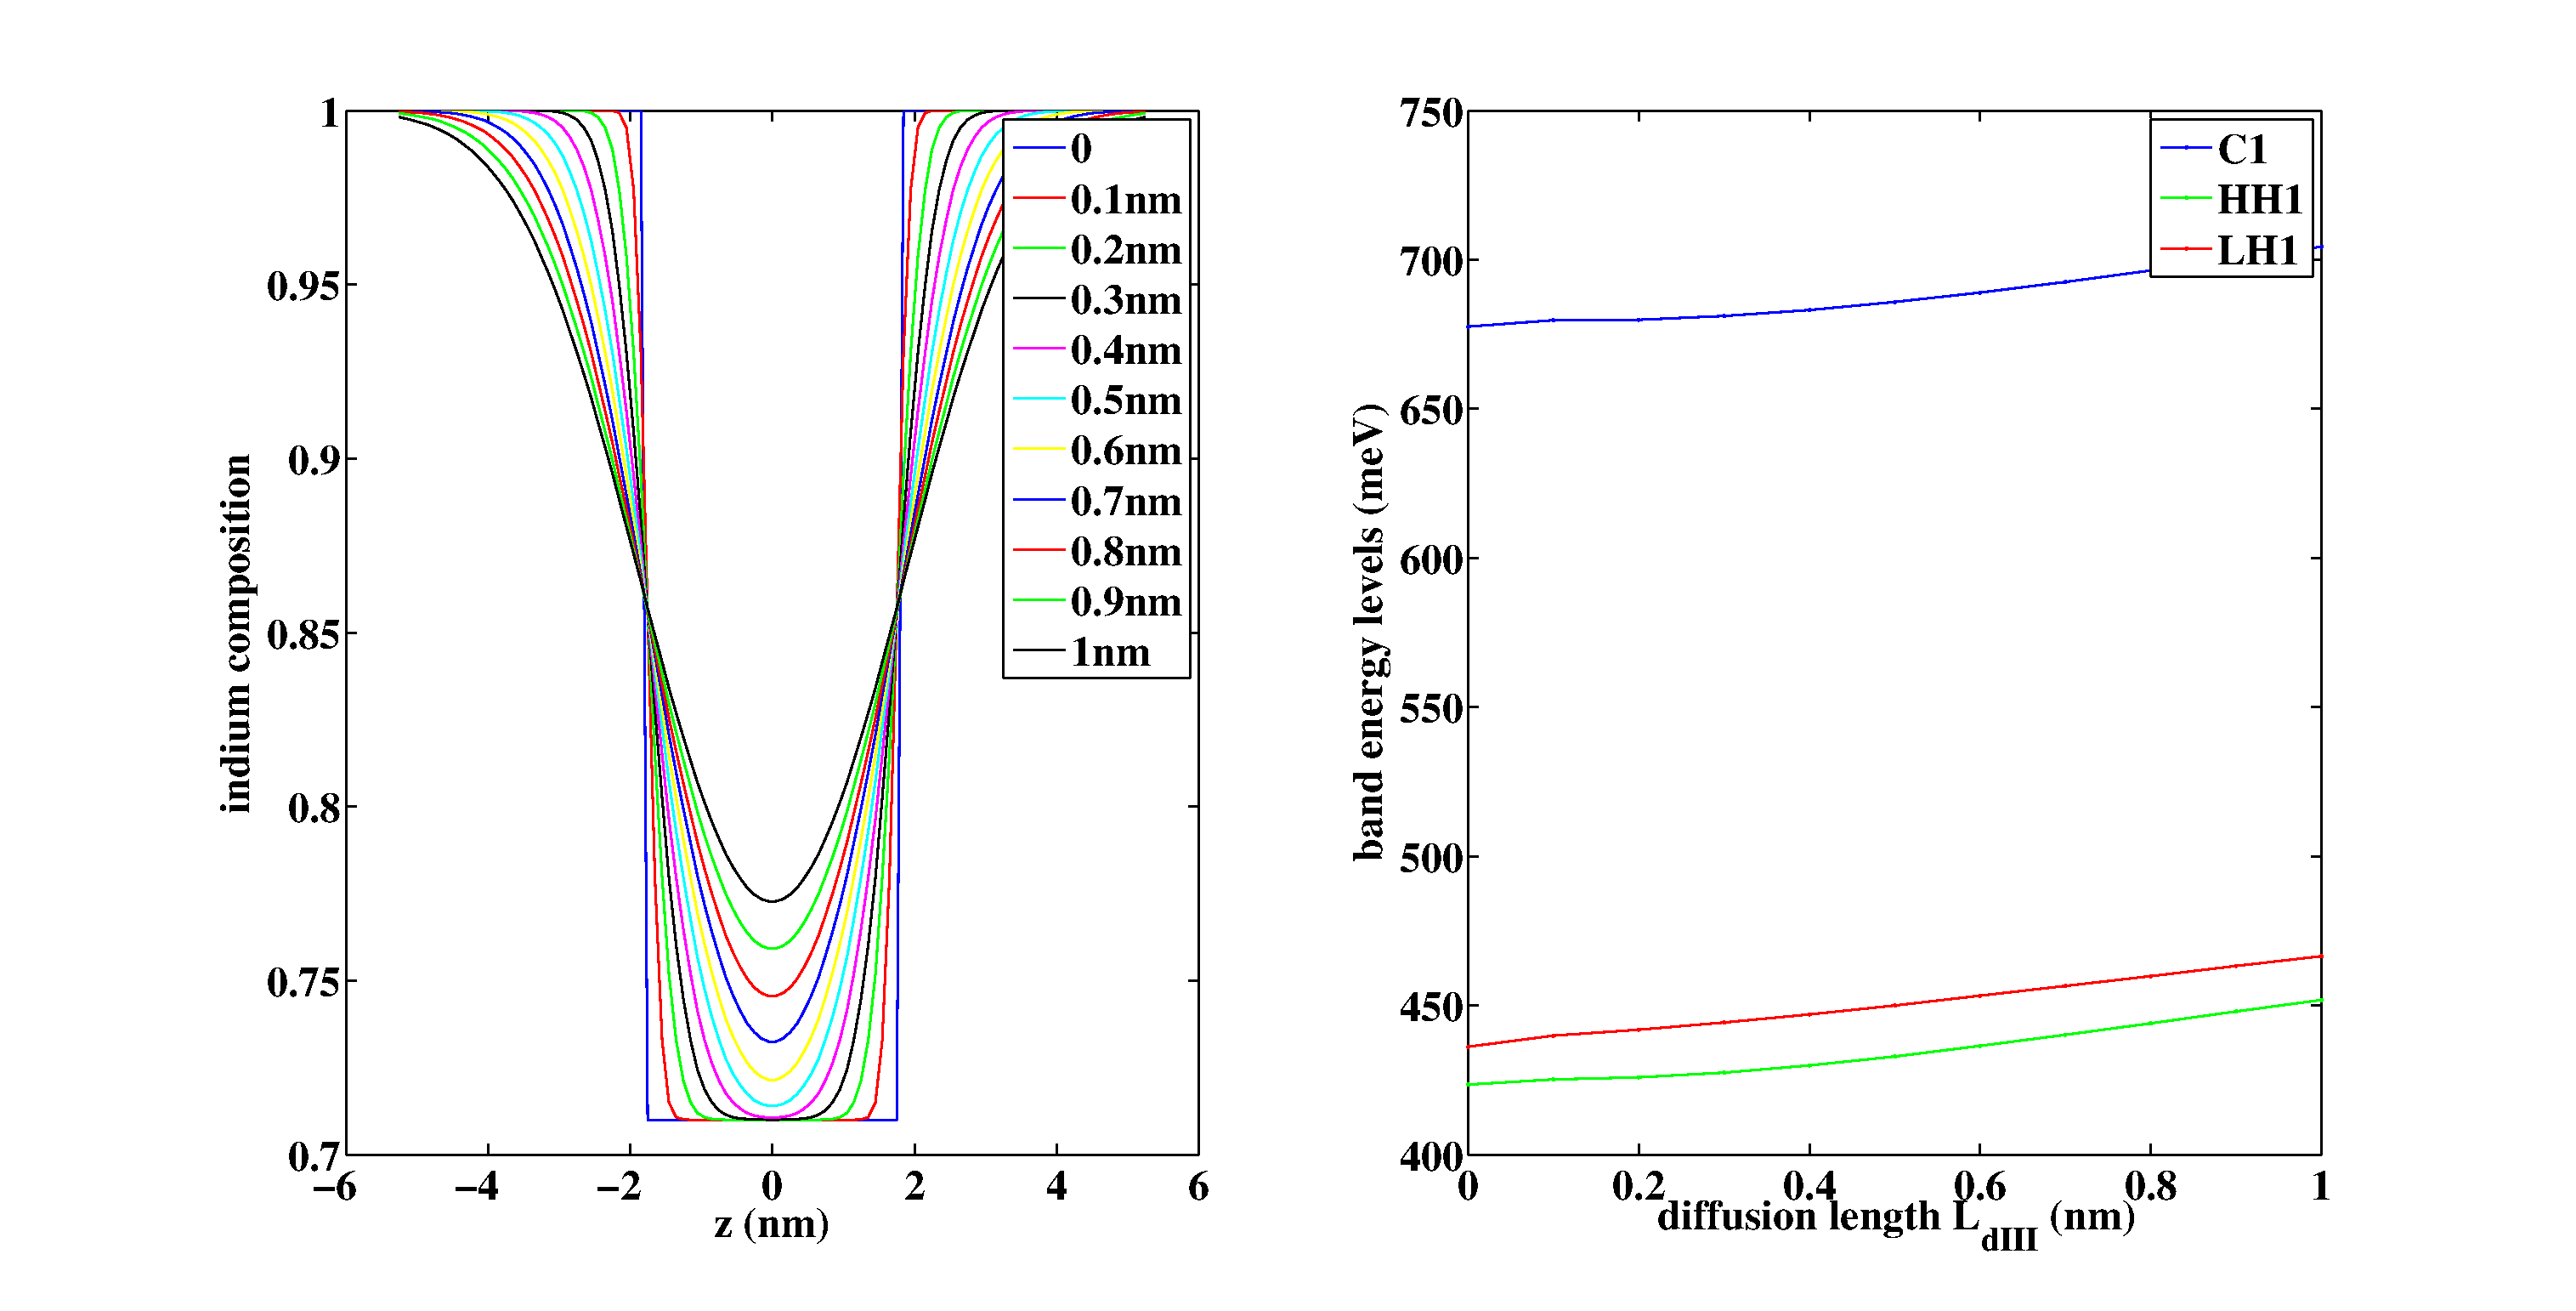
\includegraphics[width=1.0\textwidth]{./Pictures/Ld_1.eps}
    \caption{InP量子阱在不同扩散长度的条件下,导带和价带的能量变化}
    \label{fig_Ld_1}
\end{figure}

在这里,我们还可以试图将势函数的底部的能量去掉,这样一来,所有的势函数都将拥有同样的底部能量,如图~\ref{fig_Ld_2}~所示。这一次计算得到的能带的能量变化与之前的完全不同。从右边的图可以看到,在扩散长度小于0.5~nm的时候,所有能带的能量随着扩散长度的增加而增加,这个趋势和前面是相同的。这里势函数的底部能量并没有发生变化,引起能级上升的主要因素是阱宽的变化。随着扩散长度的增加,量子阱的等效阱宽在不断减小,从而导致了量子阱能级的升高。在扩散长度大于0.5~nm的时候,由于垒的势能急剧下降,导致了所有能级的能量也随之减小了。

\begin{figure}[htbp]
    \centering
    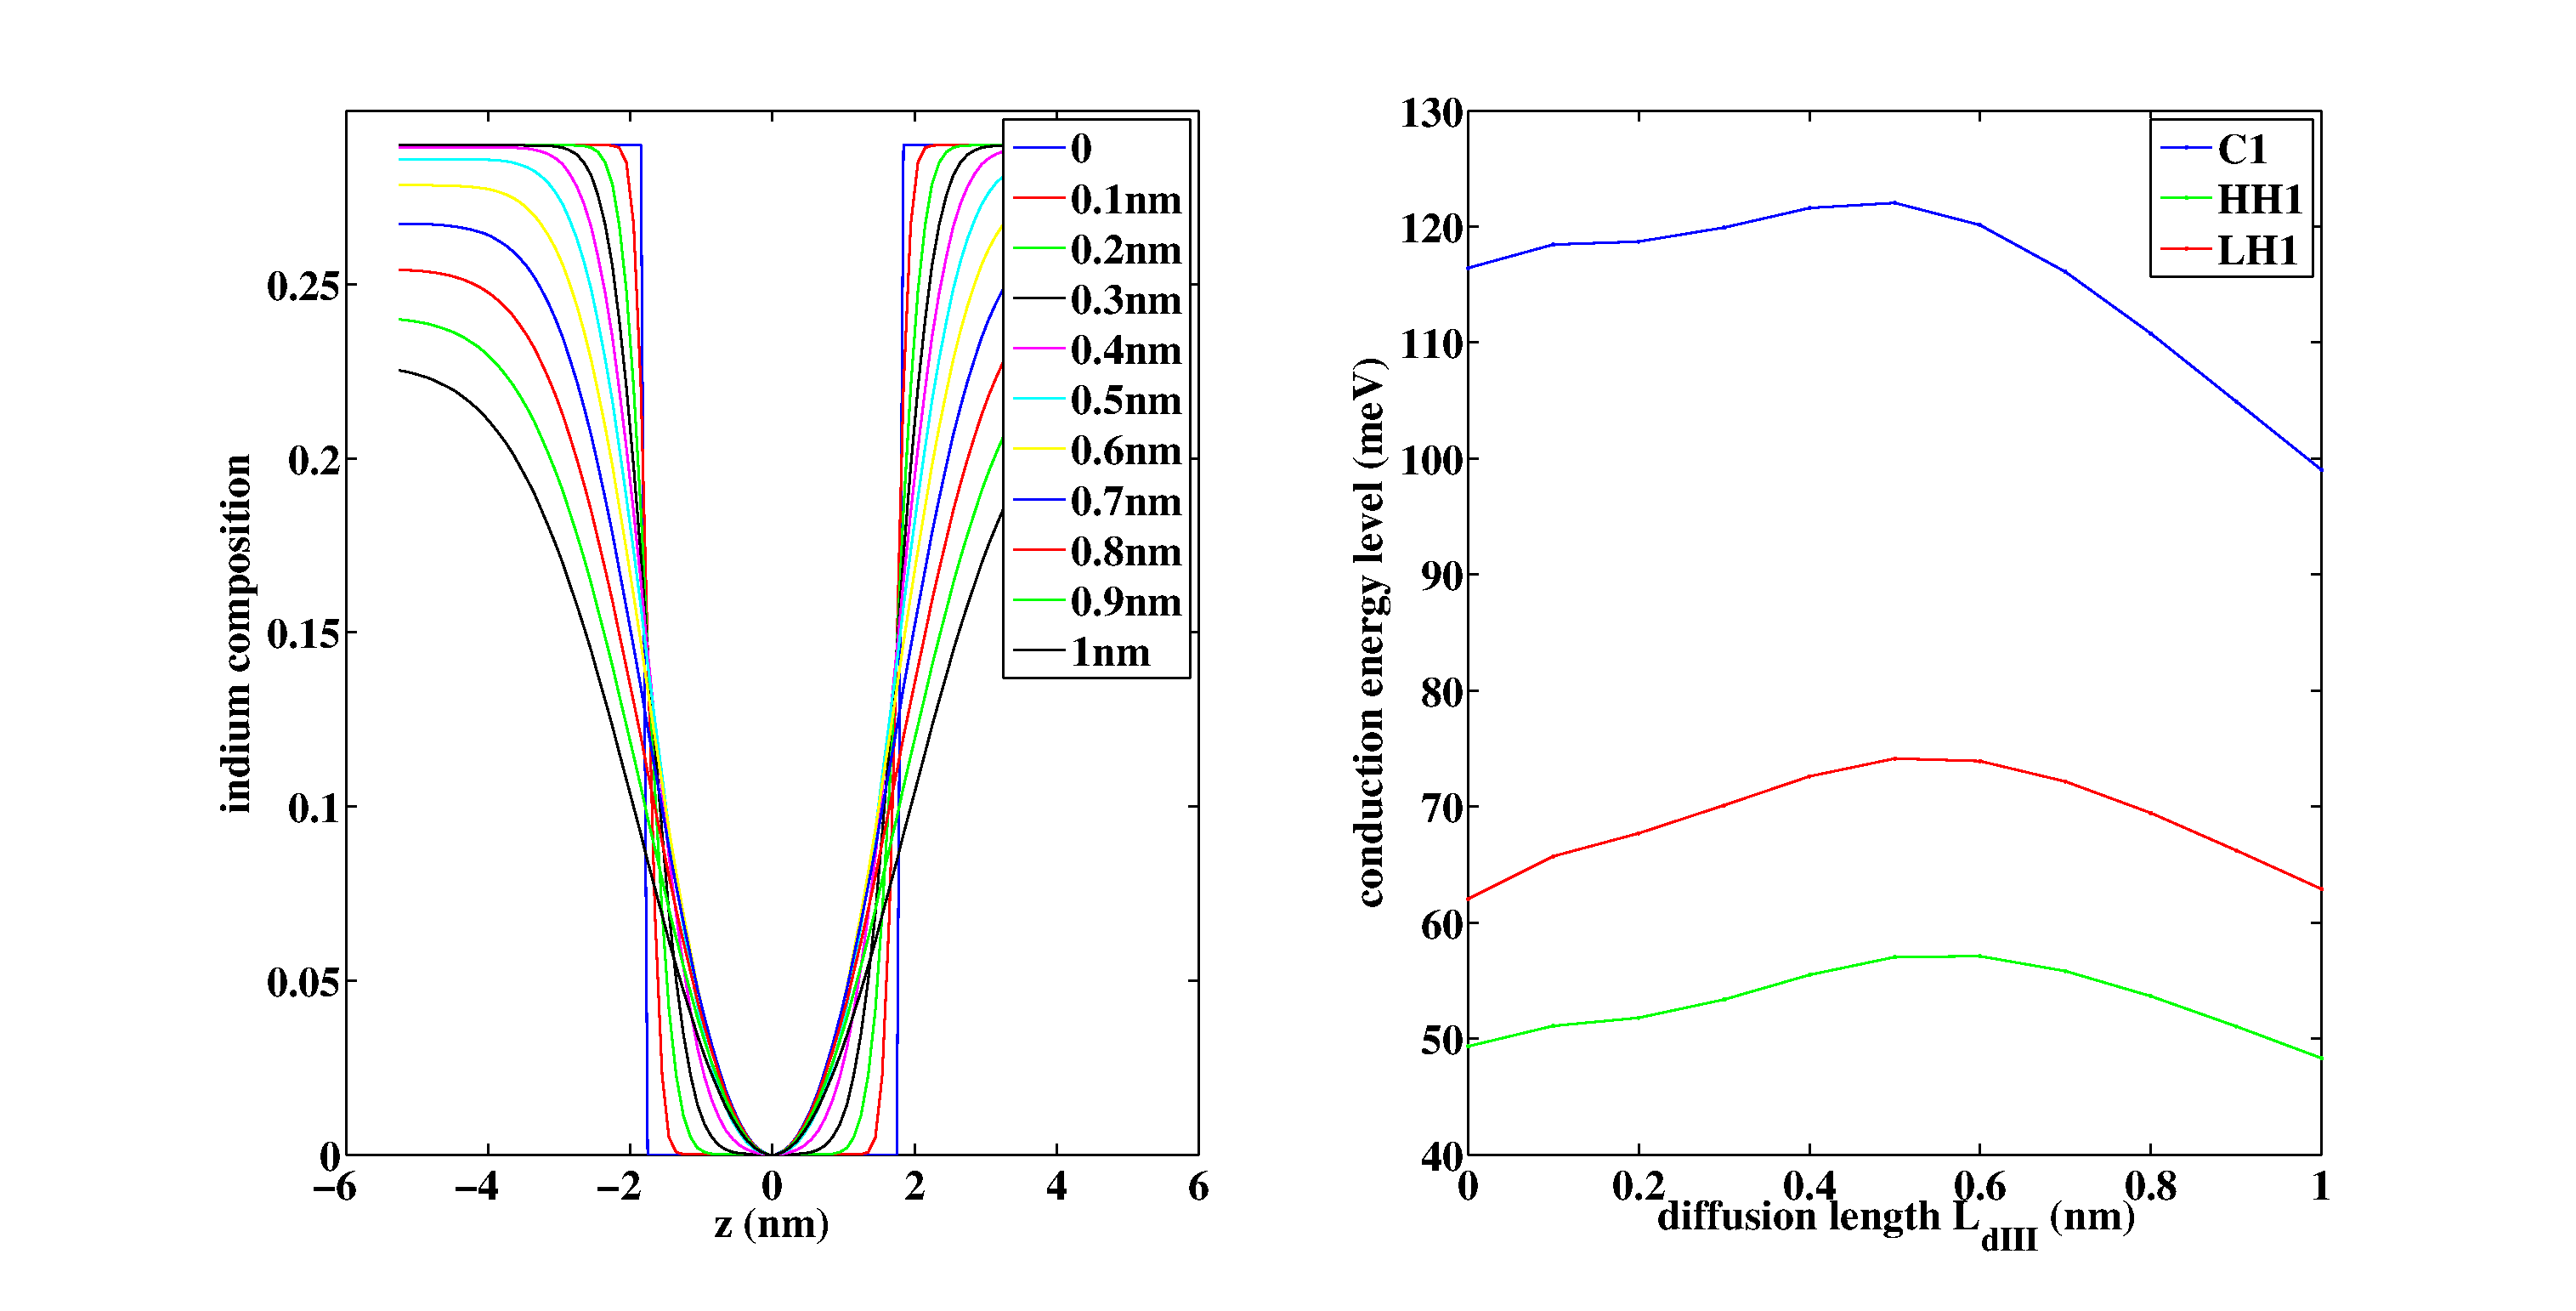
\includegraphics[width=1.0\textwidth]{./Pictures/Ld_2.eps}
    \caption{修正势函数之后的能带与扩散长度的变化关系}
    \label{fig_Ld_2}
\end{figure}

综合上述两种情况,在扩散长度比较小的情况下,阱的势能的底部还没有发生变化,这时主导能级变化的因素是等效阱宽的改变。在上面的情况中,随着扩散长度的增加,等效阱宽随之减小,这样便提升了导带和价带的能级。当扩散长度比较大时,阱的势能底部开始向上提升,垒的势能也急剧下降,他们共同导致了量子阱能级的变化。在上面的情况中,势能底的上升占据了主导地位,导致了量子阱能级随着扩散长度的增加而升高。

%%%%%%%%%%%%%%%%%%%%
\section{k值对能带结构的影响}
%%%%%%%%%%%%%%%%%%%%

除了扩散长度对蓝移会产生影响之外,k值也会影响蓝移的大小,甚至是方向。我们选择了k值为0、0.25、0.35、0.63、1的情况,分别计算C-HH和C-LH的波长变化,如图~\ref{fig_k}~左图所示。我们可以看到,当k=1时,对应的情况与上一节的情况完全相同,无论是C-HH还是C-LH的波长都一直往短波方向移动。当扩散长度达到10~nm时,蓝移可以达到200~nm以上。然而,随着k值的减小,最后能达到的蓝移也在随时减小。对于0.35和0.63两条曲线,在扩散长度大约小于2~nm的时候,波长随着扩散长度的增加而增加。之后开始向短波方向移动,并且在扩散长度小于4~nm的时候,仍然比一开始的波长要长。在4~nm之后,波长继续往短波方向移动,最终达到约100~nm左右的蓝移。对于k=0的情况,随着扩散长度的增加,波长一直向着长波方向移动,并且在最后达到约100~nm的红移。综上所述,k值越小,最后能得到的最大蓝移越小,甚至可以出现红移的现象。当k值小于一定值时,波长会出现先红移,后蓝移的现象。而k值足够小的情况下,波长会一直往红移方向移动。可见,为了在单片集成中达到尽可能大的蓝移,除了扩散长度尽可能大之外,必须尽量提高k值,即尽量加剧V族元素的扩散。如果V族元素的扩散不明显的时候,也有可能发生不蓝移,甚至红移的现象。

\begin{figure}[htbp]
    \centering
    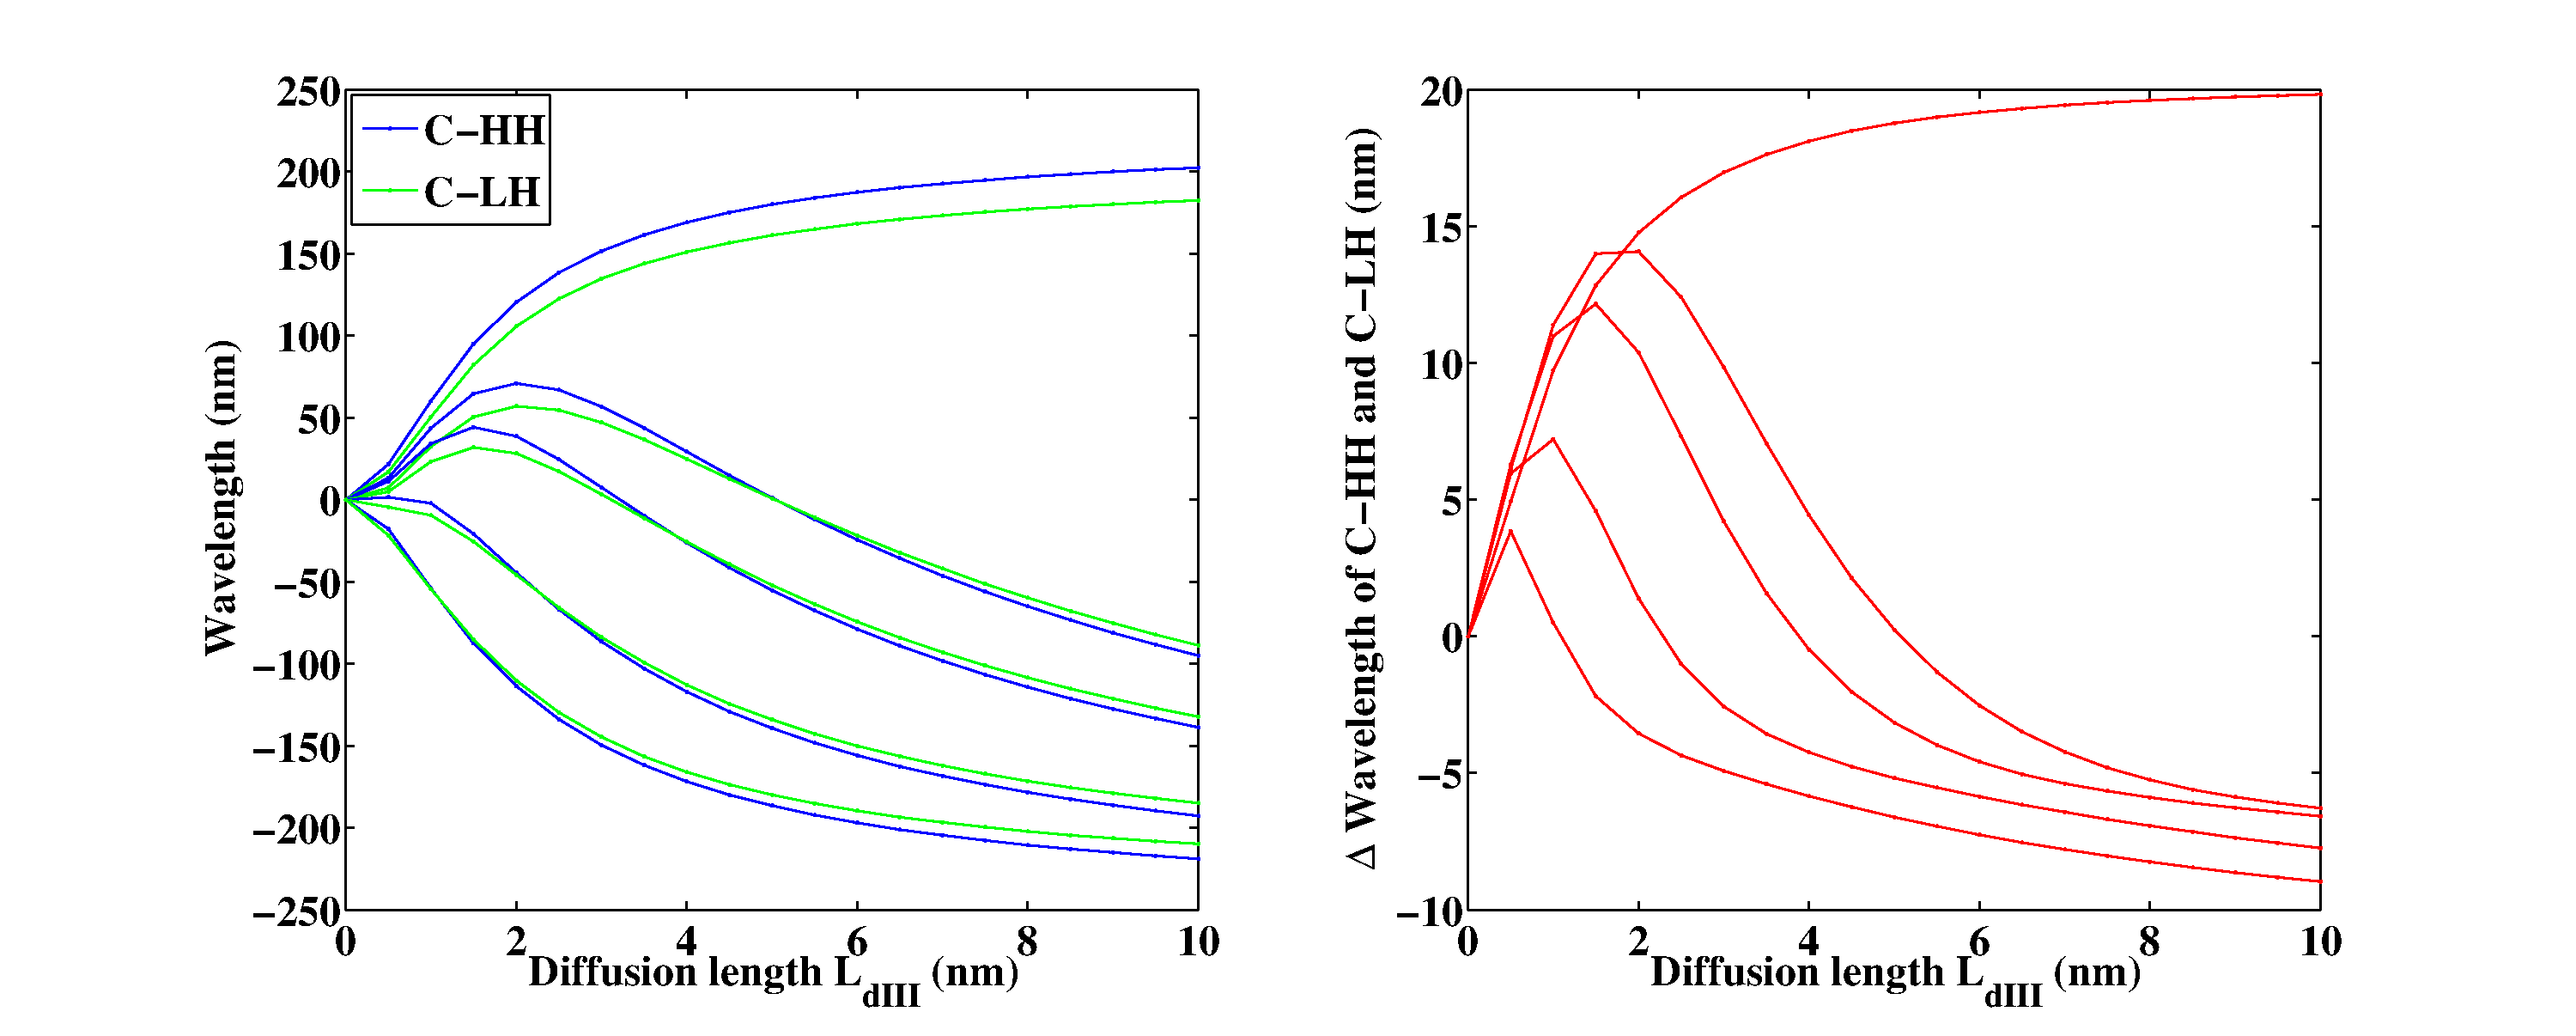
\includegraphics[width=1.0\textwidth]{./Pictures/k.eps}
    \caption{InGaAsP量子阱的C-HH和C-LH波长在不同k值和扩散长度$L_d$条件下的变化量。k值从上到下分别为0, 0.25, 0.35, 0.63, 1。}
    \label{fig_k}
\end{figure}

除此之外,我们还可以关注C-HH和C-LH变化量之间的差异,如图~\ref{fig_k}右图所示。我们可以看到,无论k值取什么值,C-HH总是可以比C-LH发生更大的变化。对于通常我们希望发生的蓝移100nm以上情况,可以发现C-HH总是可以比C-LH蓝移更大。因为C-HH主要影响TE分量,而C-LH主要影响TM分量,所以在这种情况下,TE的蓝移总是比TM大。这个结论可以用来解释量子阱混杂制作的光放大器的偏振不敏感特性。1996年,J.~J.~He等人提出了在InP量子阱材料上,用量子阱混杂方法制作的光放大器可以消除偏振敏感特性\cite{J1996Polarization},如图~\ref{fig_amplifier}~所示。在蓝移之前,TE的增益曲线对应的波长要比TM的波长大10~nm左右,而在蓝移之后,两条曲线发生了重合。这说明在蓝移的过程中,TE分量比TM分量多蓝移了10~nm左右,这与前面的描述是吻合的。

\begin{figure}[htbp]
    \centering
    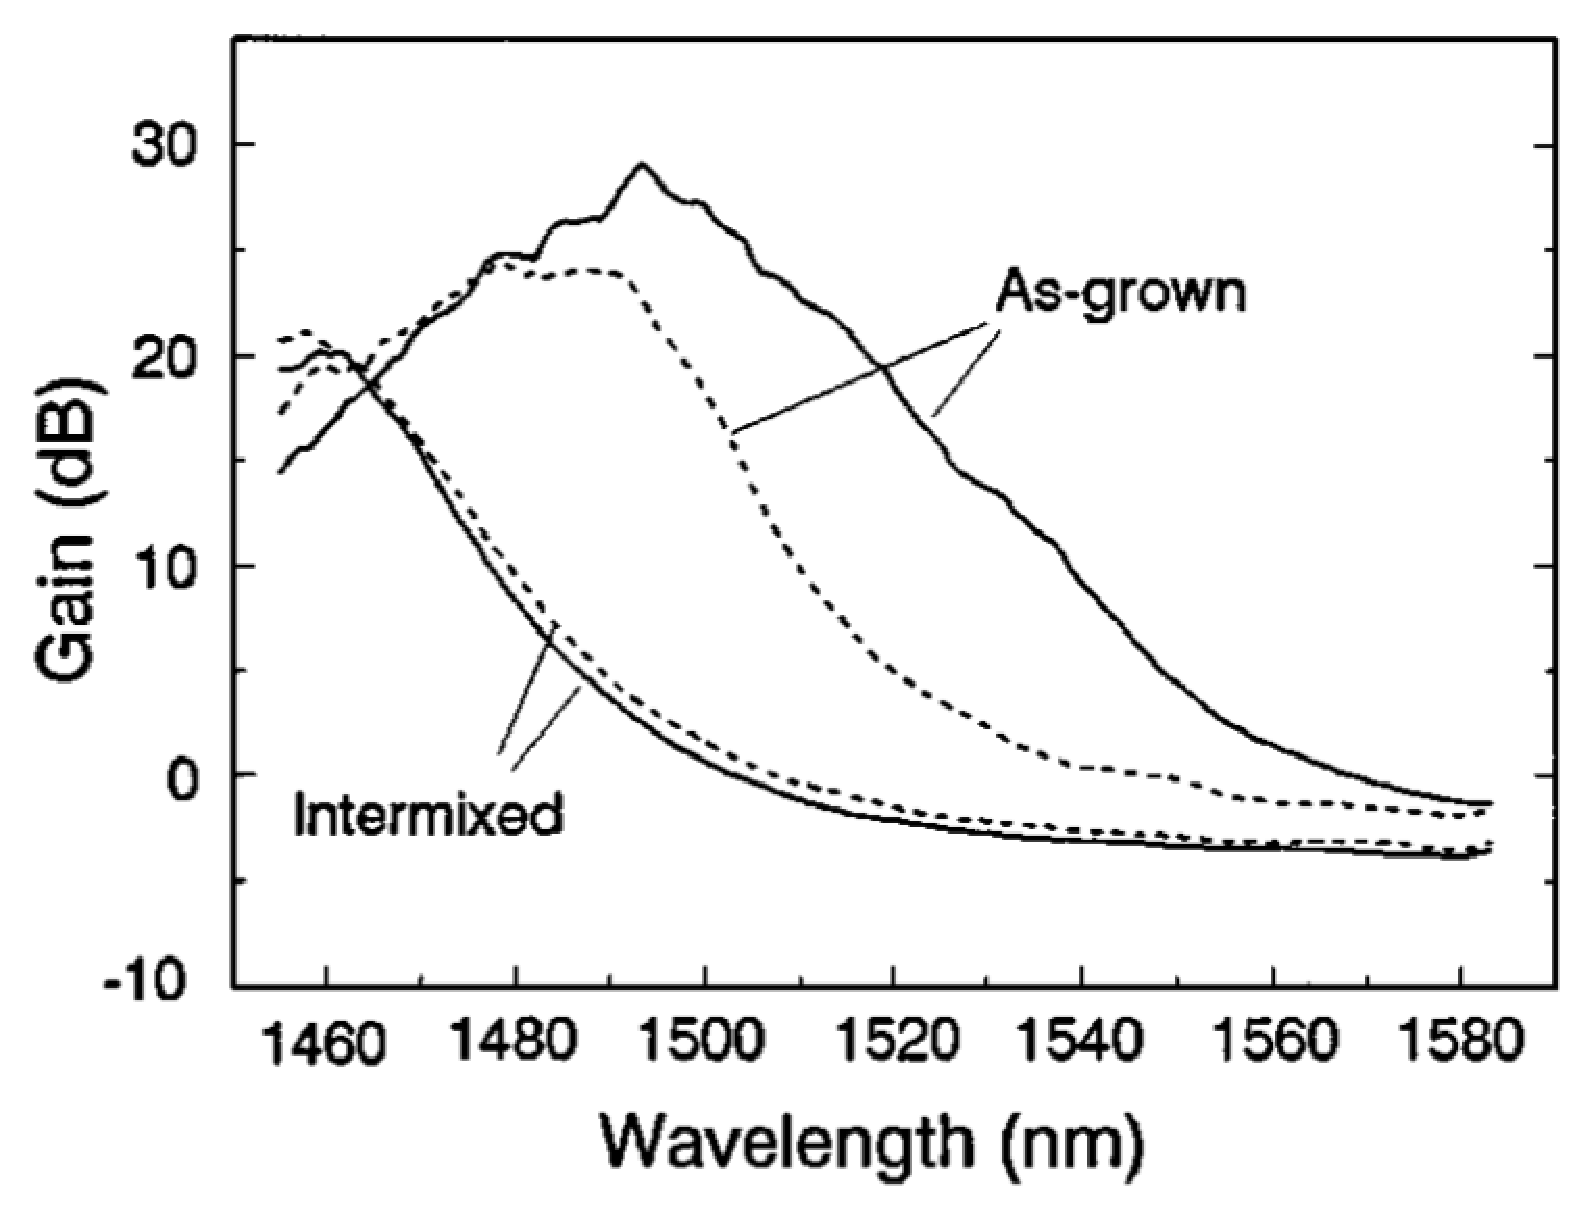
\includegraphics[width=0.5\textwidth]{./Pictures/amplifier.eps}
    \caption{测试得到的量子阱混杂之前和之后的TE和TM分量的增益曲线。其中实线表示TE分量,虚线表示TM分量。}
    \label{fig_amplifier}
\end{figure}

%%%%%%%%%%%%%%%%%%%%%%%%%%%%%%%%%%%%%%%%%%
\chapter{KrF准分子激光器照射实现量子阱混杂技术的工艺研究}
%%%%%%%%%%%%%%%%%%%%%%%%%%%%%%%%%%%%%%%%%%

%%%%%%%%%%%%%%%%%%%%
\section{实验原理}
%%%%%%%%%%%%%%%%%%%%

2004年,加拿大Sherbrooke大学的Jan J. Dubowski教授团队提出了一种新的量子阱混杂方案\cite{Genest2004UV}。他们使用KrF准分子激光器发出的248nm紫外光照射GaAs量子阱芯片的表面,然后再进行快速热退火,结果如图~\ref{fig_sherbrooke}所示。在左边的图中,随着KrF激光器能量密度的上升,GaAs量子阱片的PL的蓝移随之增加。而在右边的图中,当快速退火的温度上升到900℃之后,最大的PL蓝移达到了27nm,对GaAs量子阱材料来说已经相当可观了。这些数据表面,这种方法是完全可以达到量子阱混杂的效果的。在InP材料上,他们使用了ArF准分子激光器发出的193nm激光实现了PL波长100nm的蓝移\cite{Genest2008ArF}~。由于ArF和KrF同样是准分子激光器,只是波长相差了几十纳米,所以原理是完全相同的。

\begin{figure}[htbp]
    \centering
    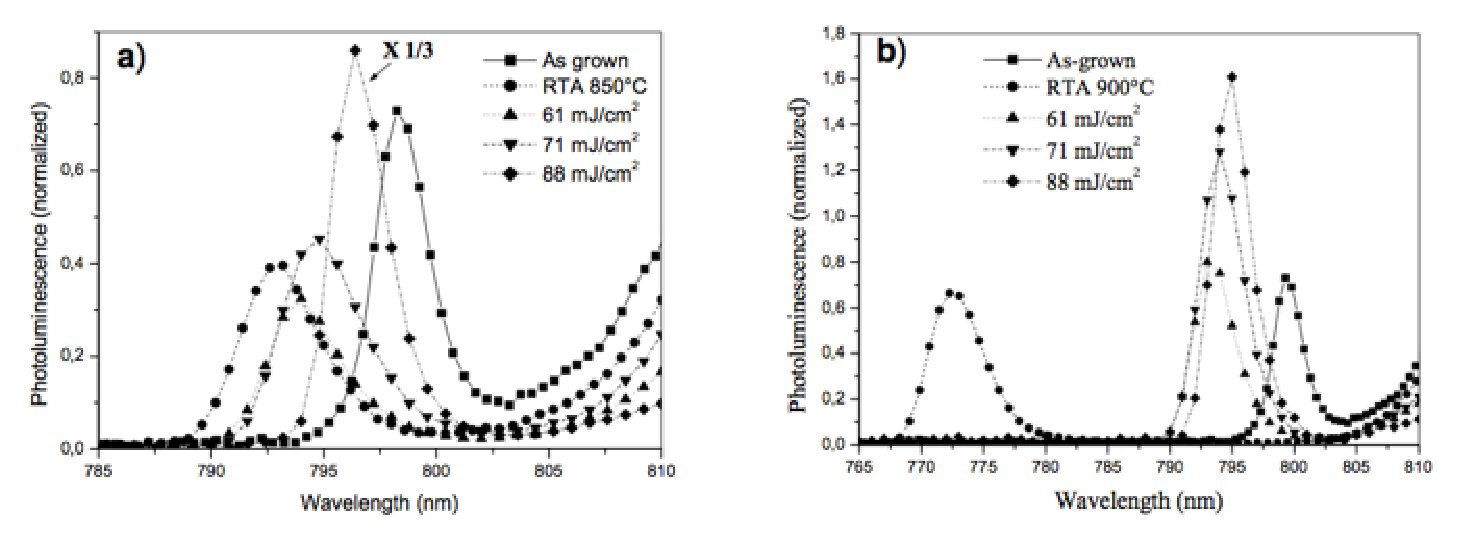
\includegraphics[width=1.0\textwidth]{./Pictures/sherbrooke.eps}
    \caption{KrF激光照射和快速热退火a)850$^{\circ}$C b)900$^{\circ}$C 之后测试得到的低温光致发光谱}
    \label{fig_sherbrooke}
\end{figure}

这种方法的其中一个优点是稳定性非常好。2015年。他们仔细研究了KrF激光器量子阱混杂方法在InP材料上的重复性,得到了PL蓝移100nm以上,同时保持标准差5.3\%的结果\cite{Beal2015Excimer}。说明这种方法将来用于工业生产也是有很大的潜力的。他们同样研究了这种方法的机理。他们将处理过的样品进行XPS测试\cite{Liu2013Chemical}。通过分析结果可以发现,KrF或ArF激光器照射过程中生成的InP$_x$O$_y$这种物质对量子阱混杂起到了决定性作用。由于原来的表面就是InP,所以新加入的O原子至关重要,换句话说,也就是在照射过程中发生了类似氧化的过程。这一点和前面篇章中讨论的阳极氧化诱导方法有些类似。当把环境中的O原子去除一部分,即放入去离子水之后,再进行同样的实验,结果发现PL蓝移从130~nm左右下降到了60~nm。这再一次证明了O原子起到了至关重要的作用。

这个方法虽然在PL蓝移上的效果很好,但是并没有应用到光器件中,波导损耗和电特性还不清楚。所以我们将利用实验室现有的设备重复并发展他们的技术。我们采用浙江大学国家重点实验室的ATLEX 300i ProMaster准分子激光器,如图~\ref{fig_promaster}~所示。其中的KrF光源发出248~nm的紫外光,能量密度0.5$\sim$5~J/cm2可调,重复频率0~300Hz可调。其中还在放置样品的地方包含了一个电动二维平移台,平移精度可以达到1~μm。

\begin{figure}[htbp]
    \centering
    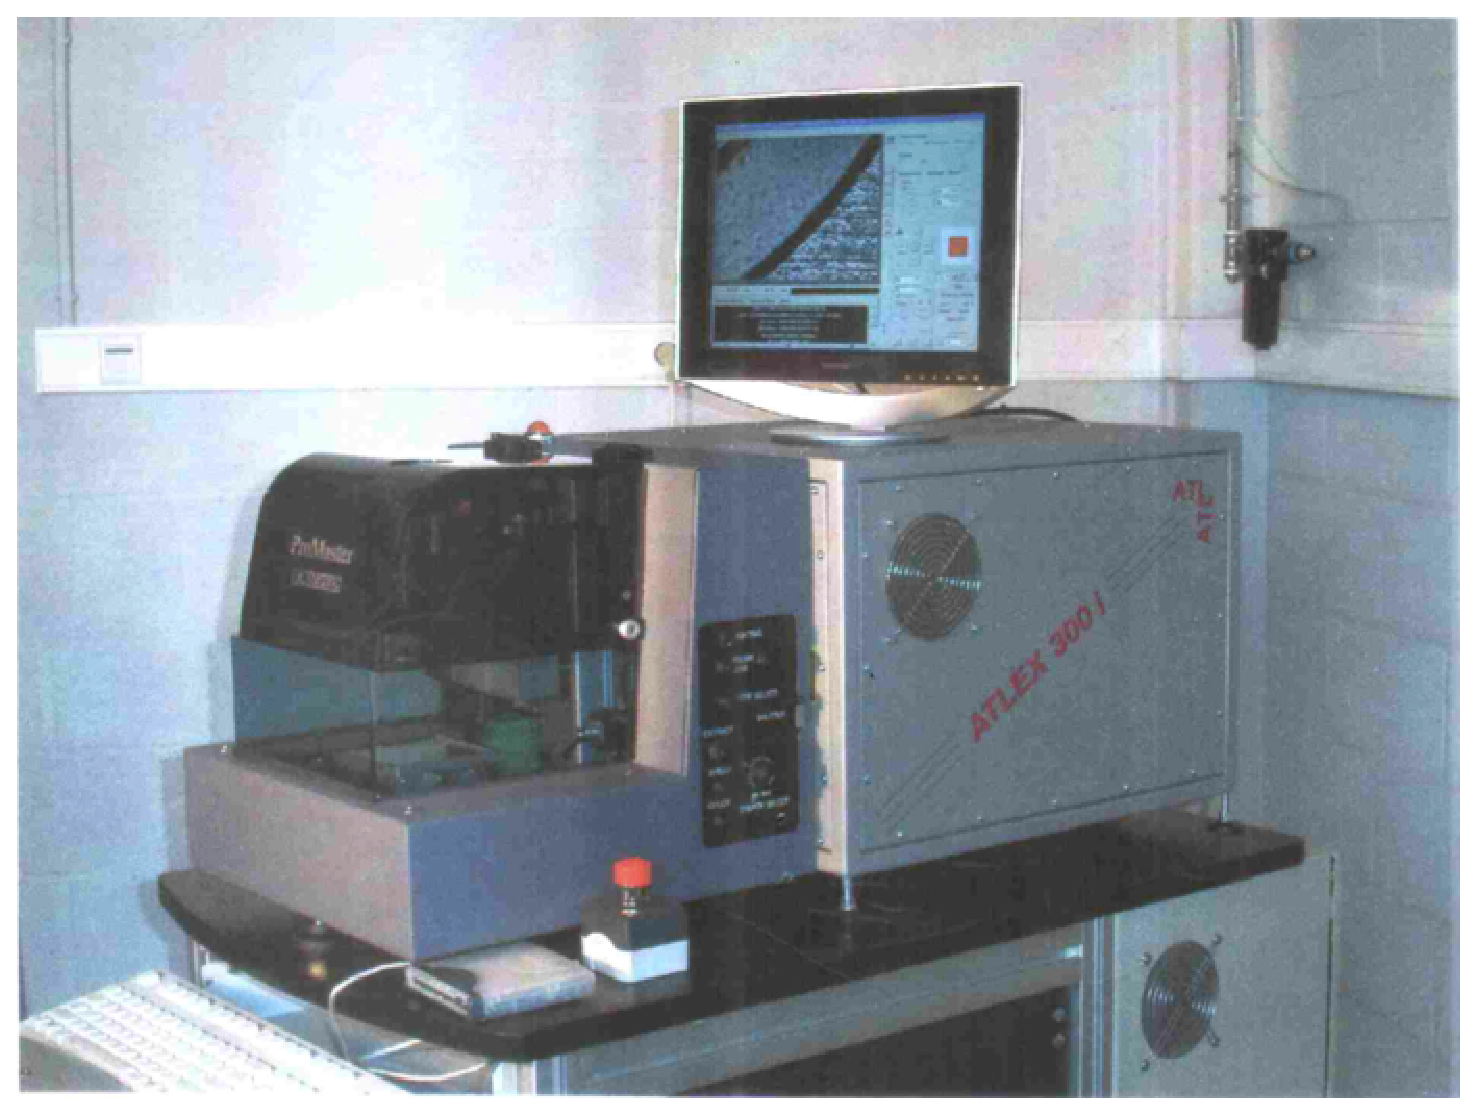
\includegraphics[width=0.7\textwidth]{./Pictures/promaster.eps}
    \caption{ATLEX 300i ProMaster准分子激光器照片}
    \label{fig_promaster}
\end{figure}

以上的参数都是符合实验要求的。但是这个设备与加拿大Sherbrooke大学的相比,有两个缺点,其一是照射面积最大只有250~μm$\times$250~μm。Sherbrooke大学的设备照射面积在1~cm$\times$1~cm以上,这样就可以一次照射到整个样品。而浙江大学的设备照射面积连他们的千分之一都不到,所以在处理比较大的样品时,必须采用扫描的方式,这样会大大增加处理的时间,降低结果的稳定性。另外一个问题是光束的均匀性很差。即使光束已经只有250~μm$\times$250~μm,但是由于没有任何匀光器等配件,光束的均匀性还是非常差。当我们将激光器的参数设置为能量密度50~mJ/cm2,脉冲数50,重复频率50~Hz,激光照射到InP芯片表面的现象如图~\ref{fig_uv_spot}~所示。在红色十字周围,有一个白色的斑,这就是紫外激光器照射在InP上面之后的痕迹。可见,这个光斑的形状是非常不规则的,长度的尺寸在200~μm左右。这样不均匀和不规则的光斑对制作复杂的集成光器件是很不利的。

\begin{figure}[htbp]
    \centering
    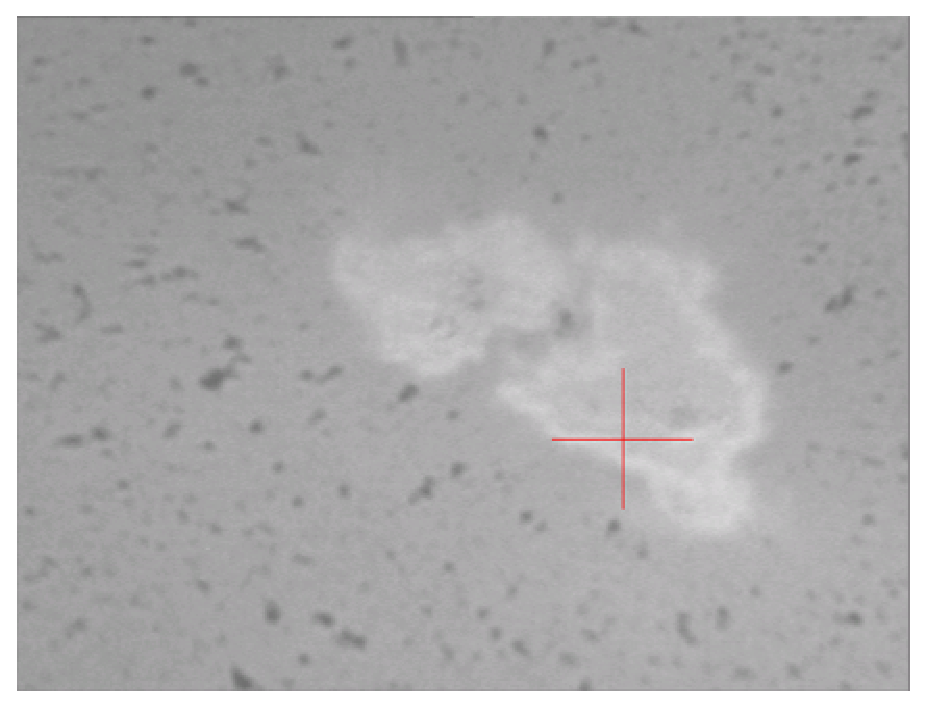
\includegraphics[width=0.7\textwidth]{./Pictures/uv_spot.eps}
    \caption{KrF准分子激光器照射一个点得到的截图}
    \label{fig_uv_spot}
\end{figure}

一个解决方案是安装非常昂贵的匀光器,我们没有采用。另一个方案是用石英掩膜板进一步减小照射的面积,这样就可以在一定程度上减轻不均匀的现象,我们采用了这个方案。当然,这样做的后果是光束更小了,处理的时间会更长。在实际的实验中,我们采用了40~μm$\times$40~μm的正方形掩膜限制了出射光斑的尺寸,使得光斑的均匀性可以接受,但是同时处理的时间大大增加了。假设要照射满一块1~cm$\times$1~cm的芯片的表面,每个40~μm$\times$40~μm的正方形的加工时间是1秒,忽略样品移动的时间,总共需要17小时以上。不过,对于一般的有源器件来说,只有一部分区域是需要进行量子阱混杂处理的,而且只占整块芯片的一小部分。所以扫描的时间完全没有这么久,还是可以接受的。

%%%%%%%%%%%%%%%%%%%%
\section{实验结果以及参数优化}
%%%%%%%%%%%%%%%%%%%%

%%%%%%%%%%%%%%%%%%%%
\subsection{实验现象与结果}
%%%%%%%%%%%%%%%%%%%%

根据前文的描述,判断量子阱混杂的好坏主要由测量蓝移前后光致发光谱的峰值波长和强度来决定。另外,由于我们使用的KrF准分子激光器的均匀性不理想,所以也需要关注材料被照射区域的均匀性。下面列出了一些主要的衡量指标:

1、混杂之后PL波长的蓝移要尽量大。

2、混杂之后的PL强度不能下降太多。

3、混杂之前PL波长的蓝移要尽量小。

4、混杂区域的空间分辨率越小越好。

5、混杂区域的PL越均匀越好。

6、去除牺牲层之后,不能观察到对材料表面的损伤。

以上六点的前四点,基本上只有通过测量PL才能得到。其中第三点主要由快速热退火的参数决定。而最后两点主要由KrF准分子激光器的参数决定。也就是说,在激光照射的时候,我们就可以通过实验现象把握混杂的均匀性和是否对材料有损伤。

图~\ref{fig_spot}~是KrF激光器照射时的操作界面。左上角区域可以看到摄像头得到的图像。其中右半边正好对焦于InP量子阱片,左半边是下面的基座。和红色的十字叉丝紧贴的方形白色区域,就是KrF激光器照射之后留下的痕迹。激光器的参数是能量密度50~mJ/cm2,脉冲数50,重复频率50~Hz。可见,当条件合适的时候,激光器照射之后的痕迹是可见的。这个痕迹呈现40~μm$\times$40~μm的方形,在摄像头下的颜色是白色。也就是说,当248~nm的紫外光照射到InP表面时,由于强度比较大,表面的材料被氧化甚至融化了。这层氧化了的材料产生了类似镜面反射的效果,所以在摄像头下显示的颜色更亮更白了。最后,我们可以看到在这个方形区域内,这种白色基本上是比较均匀的。虽然我们不能由此断定混杂之后PL也是均匀的,但是相比较之前的大光斑来说,这已经要好得多了。而对于材料的损伤,经过验证,这种白色的损伤在去掉牺牲层之后可以完全去除。说明它只存在于牺牲层里面。所以我们不妨采用这个标准作为依据,即产生一个白色的均匀的斑是KrF激光器比较理想的照射结果。

\begin{figure}[htbp]
    \centering
    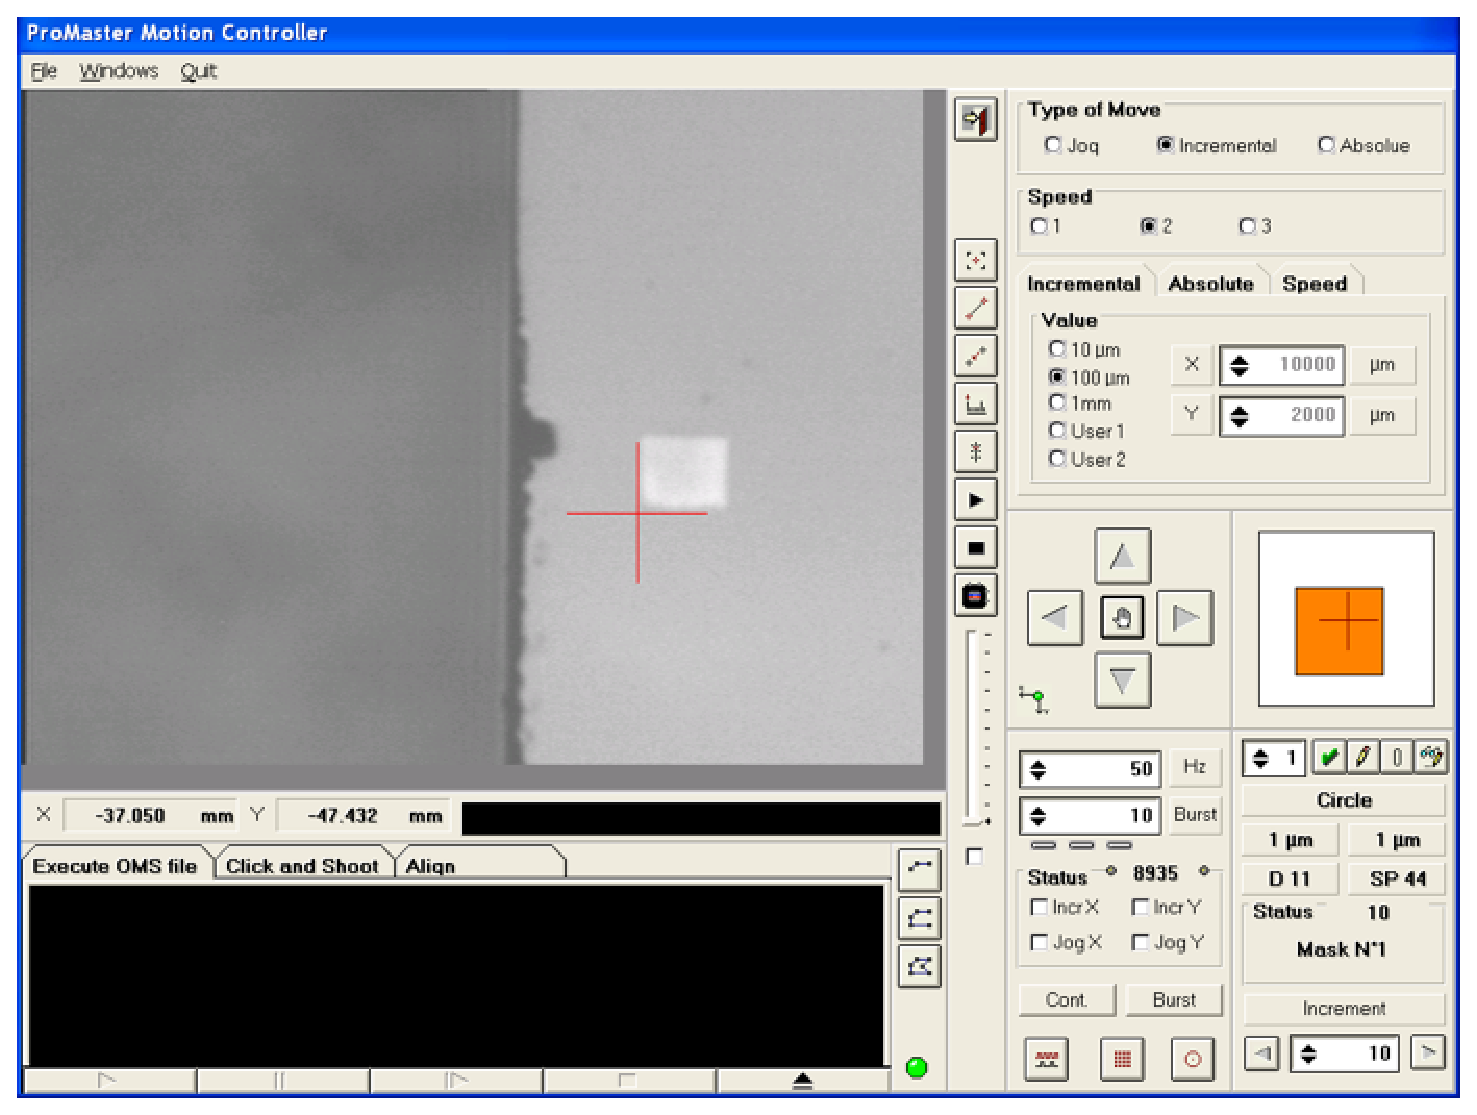
\includegraphics[width=0.7\textwidth]{./Pictures/spot.eps}
    \caption{KrF准分子激光器经过掩膜照射一个点得到的截图}
    \label{fig_spot}
\end{figure}

图~\ref{fig_spots}~是采用同一个激光器参数扫描的5$\times$5的点阵。其中相邻点的间隔是40~μm,这样就可以形成一个200~μm$\times$200~μm的大方块。从图中可以看出,每个小方块基本上可以完美地叠在一起,所以整个大方块的均匀性也是可以的。同时,所有被照射区域的颜色都呈现白色,符合前面的要求。利用这种方法,我们可以任意组合成线宽40~μm以上的各种量子阱混杂图形。一般来说,光通信的器件尺寸至少在100~μm量级,所以这个线宽是基本符合各种器件需要的。如果有更小的器件,可以在KrF激光器中更换更小的掩膜,最小可以达到5~μm,或者定做一块。

\begin{figure}[htbp]
    \centering
    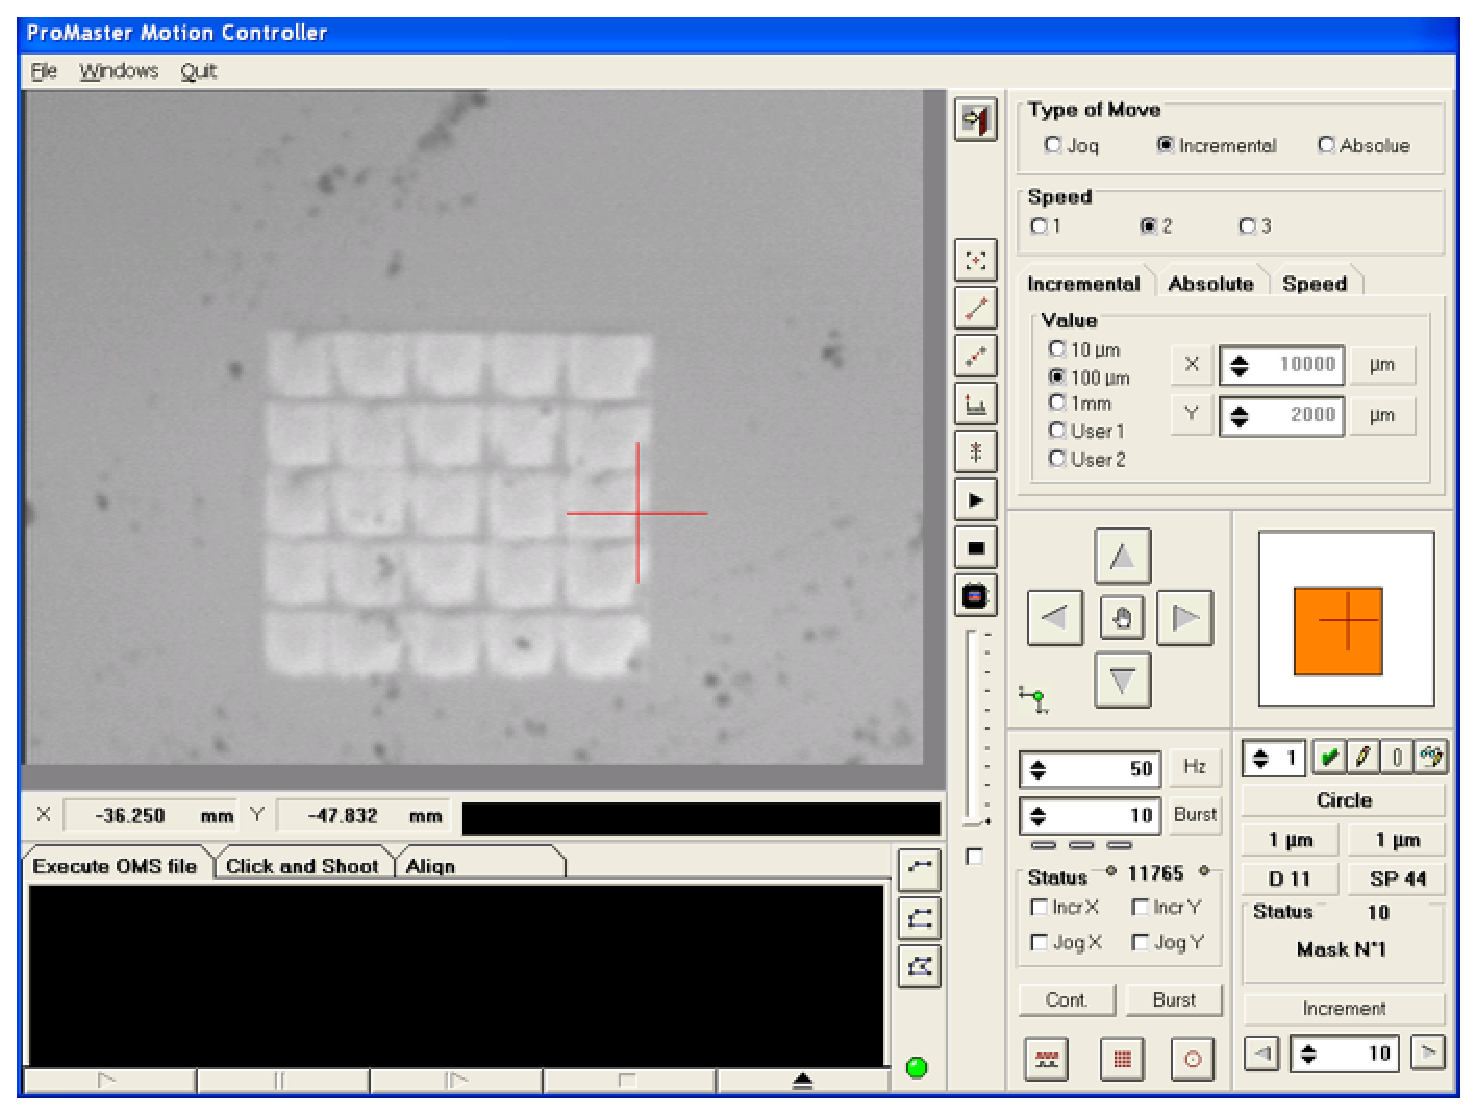
\includegraphics[width=0.7\textwidth]{./Pictures/spots.eps}
    \caption{KrF准分子激光器照射5×5点阵得到的截图}
    \label{fig_spots}
\end{figure}

然后,我们将这块样品放入快速热退火炉中处理,退火的温度是750$^{\circ}$C,时间90秒。在退火炉中,为了保护芯片不被氧化,高纯度氮气被不断冲入退火炉中。同时,芯片的正反面同时由两块新的硅片夹住,这样可以有效防止InP牺牲层中的P原子在高温条件下析出\cite{Pearton1990Reproducible}\cite{Hulko2006The}。退火完成之后,芯片表面的InP牺牲层用HCl:H2O=3:1的溶液腐蚀掉。最后,样品在PL测试台上进行测试,结果如图~\ref{fig_uv_result}~所示。其中,原生片PL的波长峰值在1550~nm附近,而只做退火芯片的PL蓝移到1525~nm附近,强度略微下降5\%左右。在750$^{\circ}$C条件下这种现象是完全正常的。而对于量子阱混杂的芯片,PL峰值波长蓝移到了1390~nm附近,净蓝移135~nm,这个蓝移是比较大的。同时强度上升了20\%左右,说明量子阱混杂之后,量子阱芯片的质量反而上升了。上升的原因除了和本身的能带结构有关之外,另一种解释是芯片在量子阱混杂之前本身含有很多缺陷。这些缺陷在混杂的过程中运动到了芯片的基底中,使得芯片的质量变好了。在Sherbrooke大学的实验中,也出现过PL强度上升的现象\cite{Liu2013Enhanced}。总之,无论是蓝移还是强度,都表明这种量子阱混杂的方法的效果是比较理想的。

\begin{figure}[htbp]
    \centering
    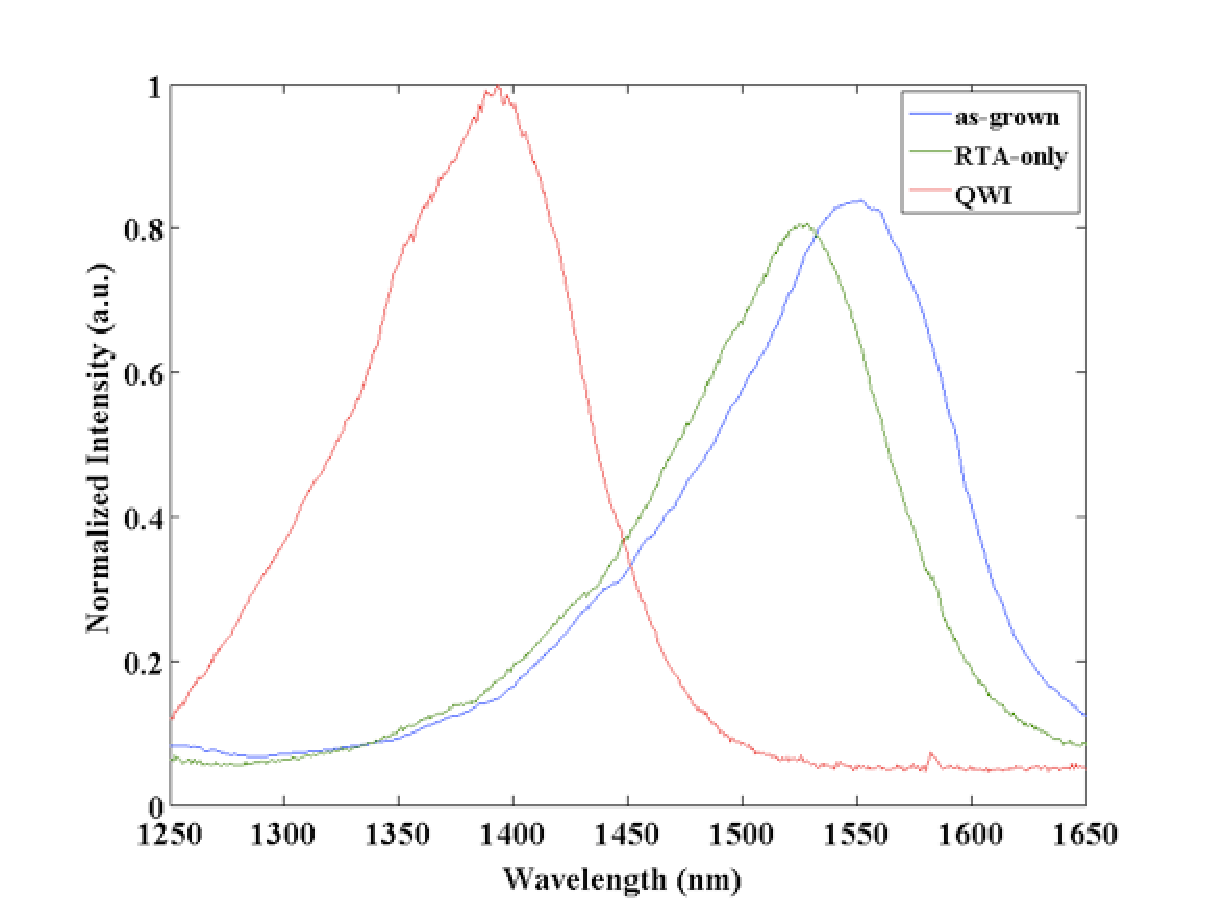
\includegraphics[width=0.7\textwidth]{./Pictures/uv_result.eps}
    \caption{在750$^{\circ}$C,90s的快速热退火条件下的PL与只做退火和原生片PL的对比}
    \label{fig_uv_result}
\end{figure}

%%%%%%%%%%%%%%%%%%%%
\subsection{快速热退火对结果的影响}
%%%%%%%%%%%%%%%%%%%%

我们首先讨论快速热退火对结果的影响。由于混杂的均匀性和对芯片的损伤基本上由KrF激光照射的时候决定,所以我们这里只讨论快速热退火对蓝移前后PL的影响。

快速热退火主要由退火温度和时间两个参数决定。这里我们首先分析只做退火的芯片在不同退火温度条件下的PL的变化趋势,如图~\ref{fig_heat_stability}~所示。从图中可以看出,在退火时间稳定在90~s的条件下,随着退火温度从725$^{\circ}$C开始逐渐上升到750$^{\circ}$C和775$^{\circ}$C,PL峰值波长也随之蓝移到1540~nm、1530~nm和1516~nm。说明随着温度升高,蓝移也在增加。同时强度也分别下降到了原生片的98\%、95\%和90\%左右。也就是随着温度的升高,强度不断下降。然后,我们对这三个温度,各取30~s、60~s和90~s三个时间进行退火,结果如图~\ref{fig_heat_stability_shift}~所示。从图中可以看出,对于这三个温度,随着退火时间增加,蓝移都随之增加了。当退火时间增加到90~s时,净蓝移相对于60~s时已经变化不大,分别为5~nm、20~nm和34~nm,趋向于饱和。所以,为了保证每次只做退火区域的波长相对稳定,我们需要取60~s以上为退火时间。因为再加长时间对蓝移并没有贡献,反而会进一步减小PL强度。而取多高的退火温度,主要由量子阱混杂的结果决定。

\begin{figure}[htbp]
    \centering
    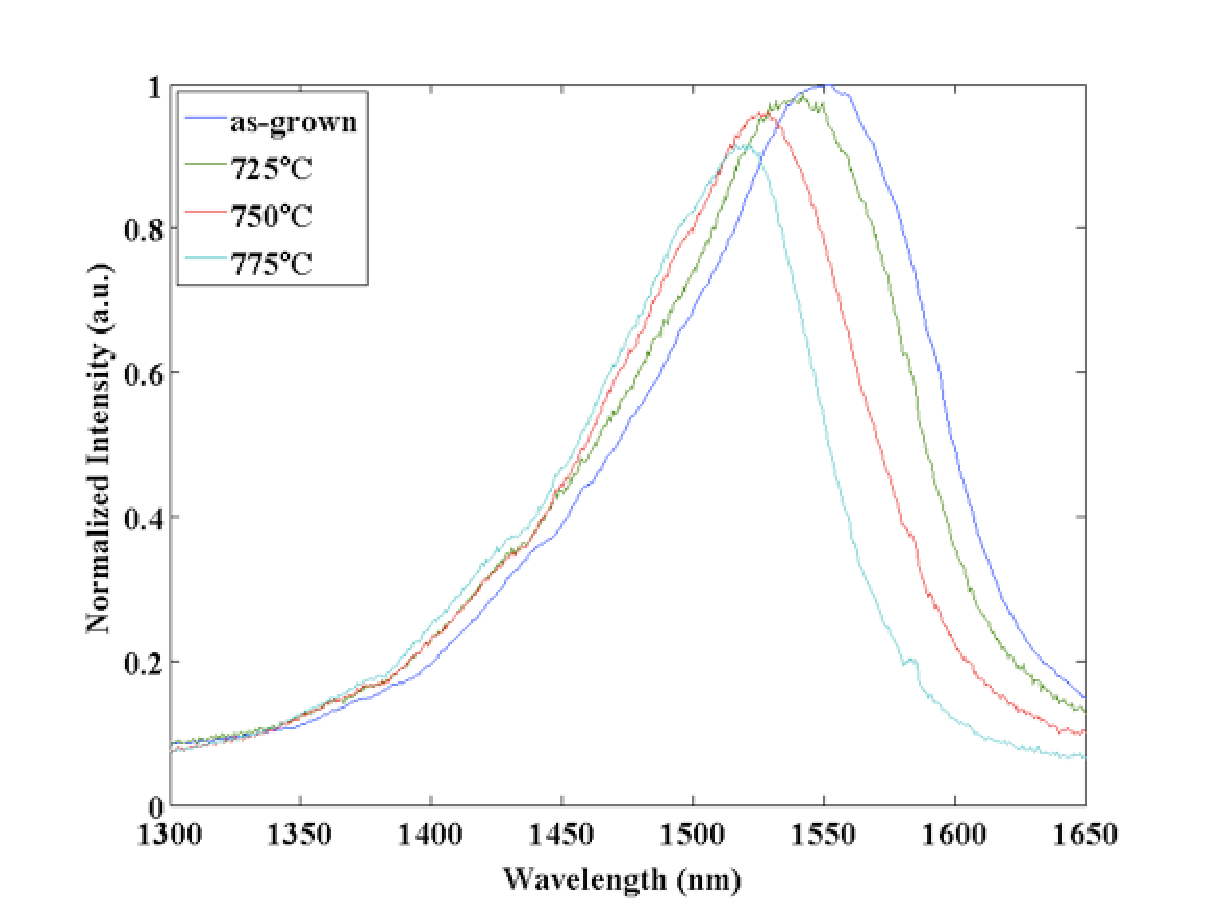
\includegraphics[width=0.7\textwidth]{./Pictures/heat_stability.eps}
    \caption{只做退火的InP量子阱片在725$^{\circ}$C、750$^{\circ}$C和775$^{\circ}$C快速热退火条件下的PL与原生片PL的对比}
    \label{fig_heat_stability}
\end{figure}

\begin{figure}[htbp]
    \centering
    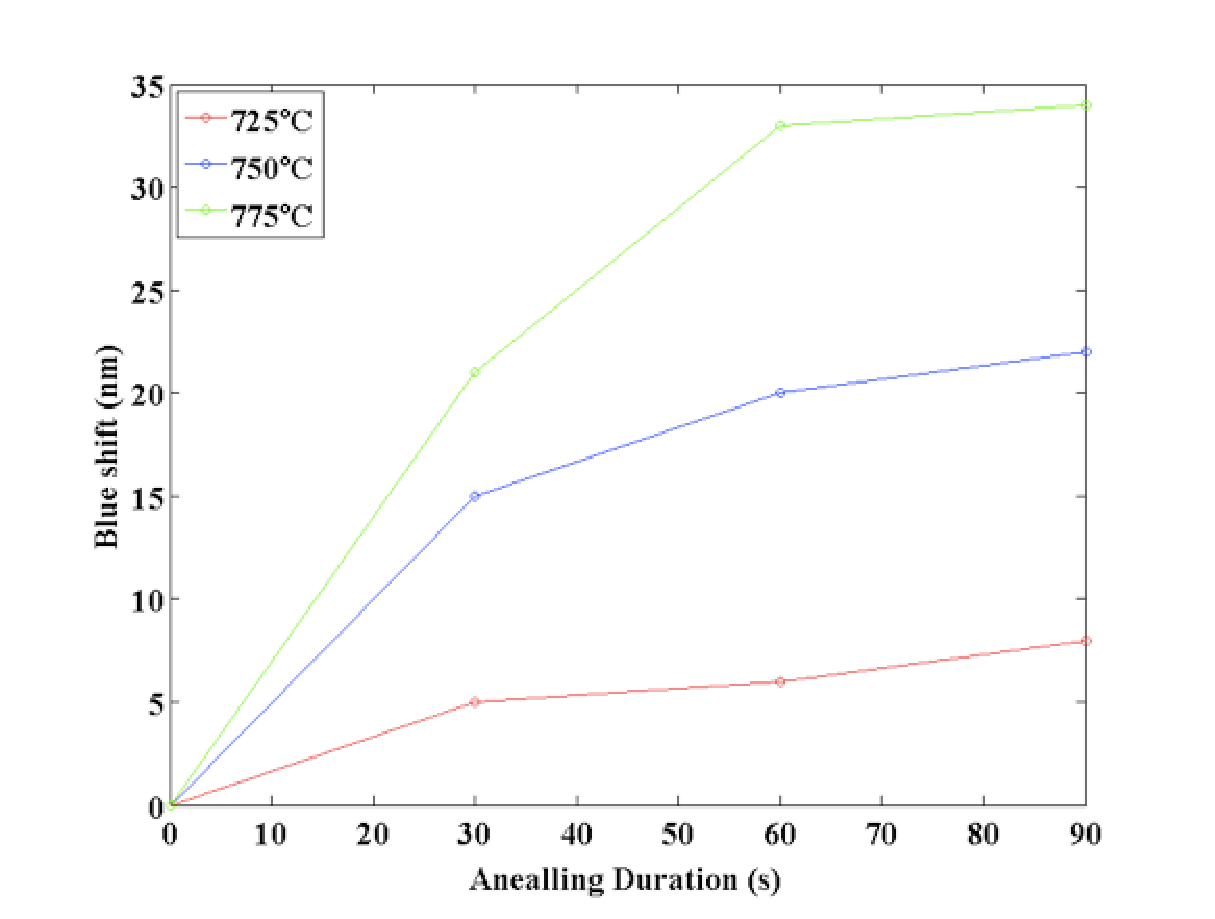
\includegraphics[width=0.7\textwidth]{./Pictures/heat_stability_shift.eps}
    \caption{只做退火的InP量子阱片在不同温度和时间的快速热退火条件下的PL峰值波长净蓝移}
    \label{fig_heat_stability_shift}
\end{figure}

相似地,我们对经过KrF激光照射的芯片也用不同的退火温度和时间处理,结果如图~\ref{fig_qwi_rta}~所示。其中KrF激光参数统一为50~J/cm2,50脉冲,50~Hz。从图中可以看出,决定净蓝移的最重要因素是退火温度。随着温度的增加,净蓝移也随之增加。同时,对于每一个温度,当退火时间增加之后,净蓝移也随之增加。而时间增加到90~s以上时,净蓝移稳定在80~nm、135~nm和170~nm左右,趋于饱和。这说明为了让每次的净蓝移结果相对稳定,可以取90~s以上为退火时间。对于退火温度选择可以依实际情况而定。如果需要制作完全无源区域,则需要净蓝移在100~nm以上,那么退火温度在750$^{\circ}$C或以上比较合适。如果是电吸收调制器,蓝移在50~nm$\sim$70~nm范围内比较合适,那么725$^{\circ}$C也是偏高的,需要进一步减小退火温度。

\begin{figure}[htbp]
    \centering
    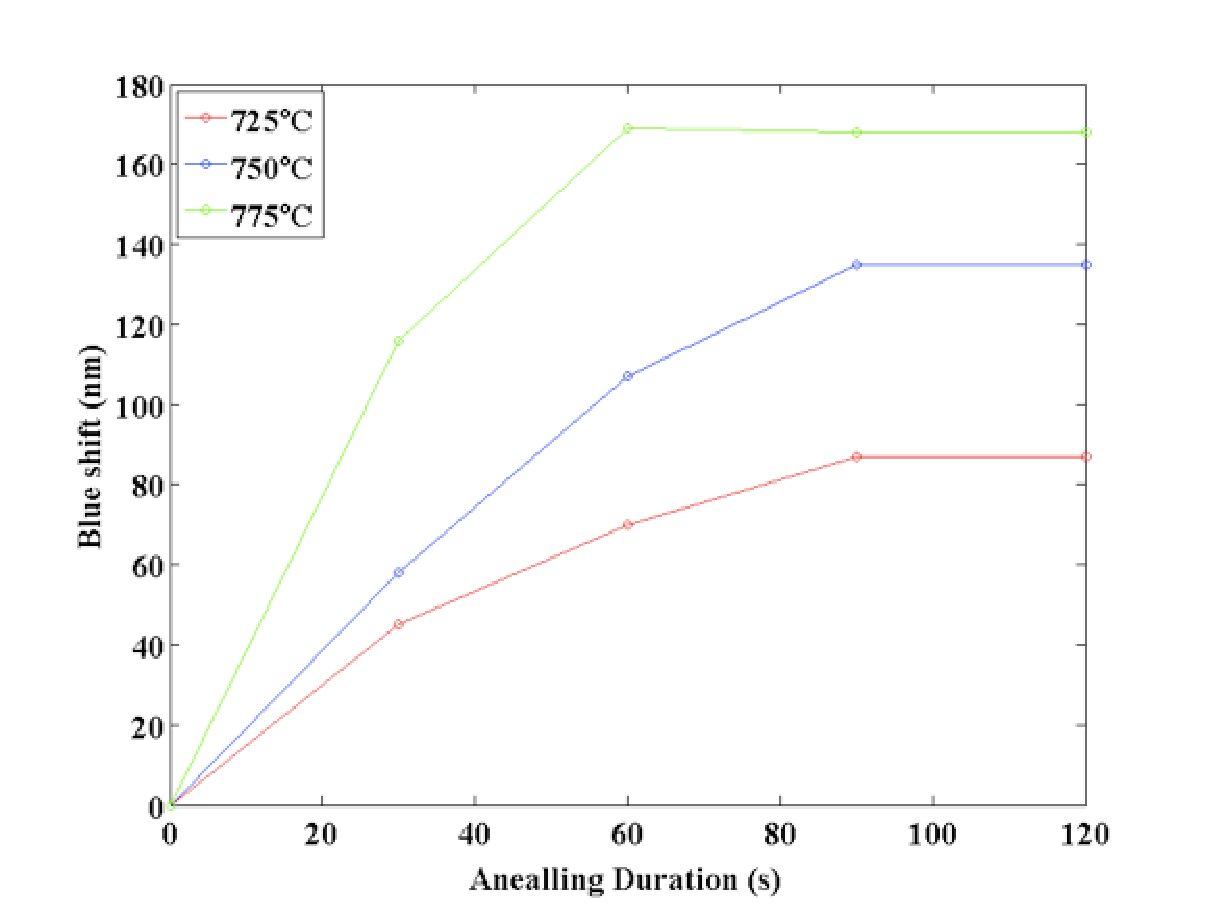
\includegraphics[width=0.7\textwidth]{./Pictures/qwi_rta.eps}
    \caption{量子阱混杂的InP量子阱片在不同温度和时间的快速热退火条件下的PL峰值波长净蓝移}
    \label{fig_qwi_rta}
\end{figure}

图~\ref{fig_qwi_725C}~给出了725$^{\circ}$C、90秒条件下的PL与制作退火和原生片PL的对比。从图中可以看出,在量子阱混杂之后,PL的波长蓝移到1460~nm左右,净蓝移80~nm。同时PL强度上升了大约30\%。这些结果与图~\ref{fig_uv_result}~中的750$^{\circ}$C条件下的结果是相似的。只是温度小一些,蓝移也小一些。图~\ref{fig_qwi_775C}~是775$^{\circ}$C条件下的结果。其中波长蓝移到1350~nm左右,净蓝移约170~nm。强度也上升了10\%。以上结果表明,这三个温度下的PL都发生了明显的蓝移,同时强度都上升了。其中750$^{\circ}$C和775$^{\circ}$C的蓝移都在100~nm以上,符合制作无源材料的要求。同时,随着温度的升高,PL强度的增加量分别为30\%、20\%和10\%左右,说明更高的温度会导致PL下降的趋势。所以。在蓝移足够的情况下,应该尽量降低退火的温度。所以在下面的研究中,我们将退火的参数固定在750℃和90秒。值得一提的是,这两张图中在1375~nm左右都出现了肩峰,这是测试系统的谐波造成的。

\begin{figure}[htbp]
    \centering
    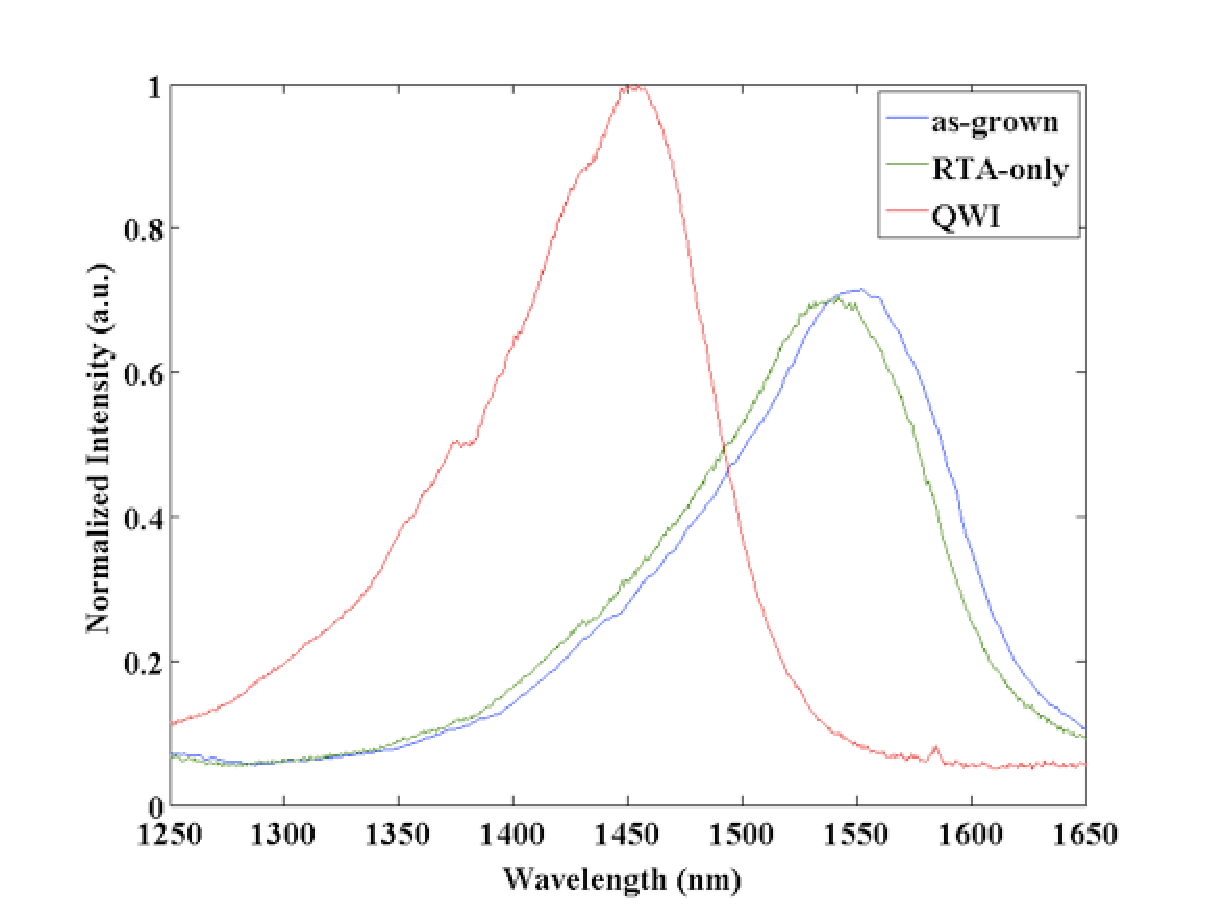
\includegraphics[width=0.7\textwidth]{./Pictures/qwi_725C.eps}
    \caption{在725$^{\circ}$C,90s的快速热退火条件下的PL与只做退火和原生片PL的对比}
    \label{fig_qwi_725C}
\end{figure}

\begin{figure}[htbp]
    \centering
    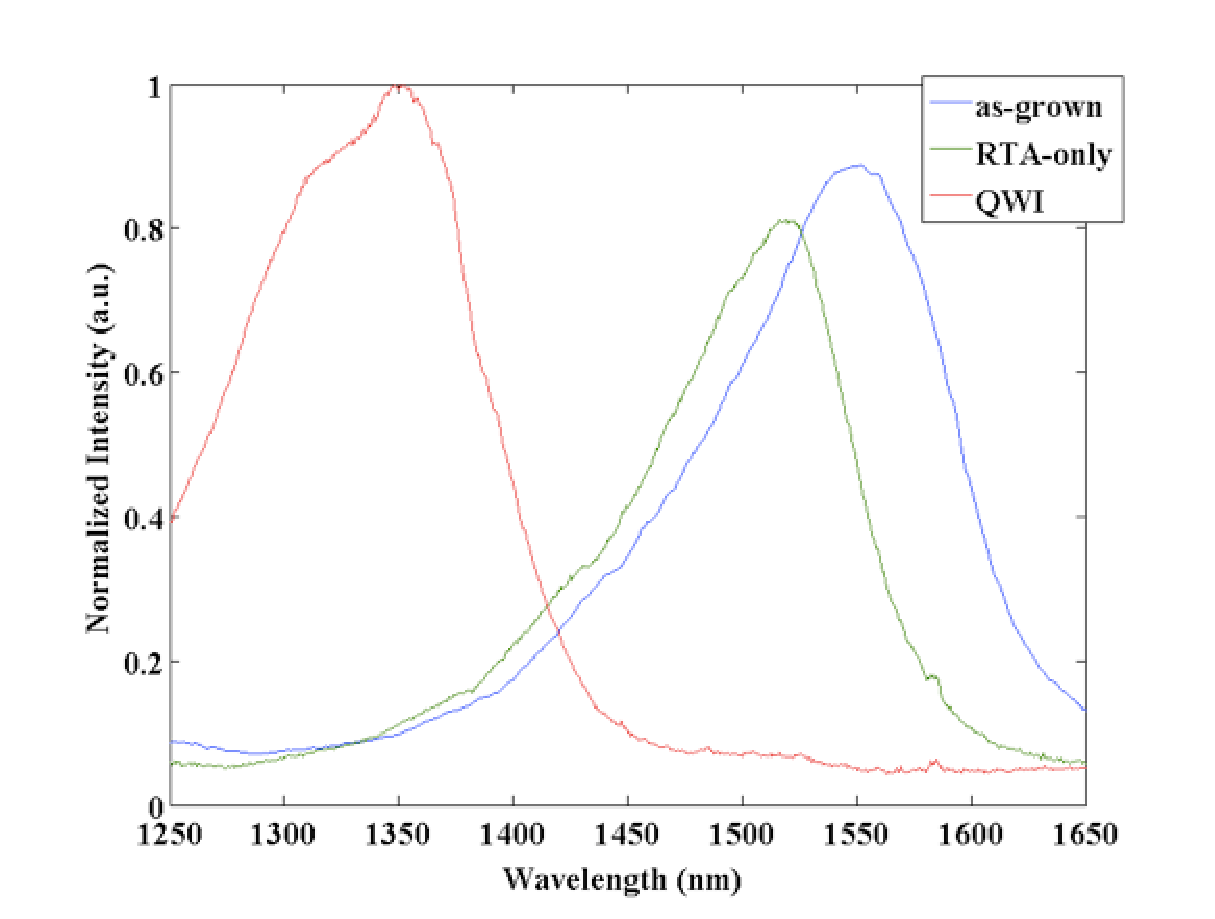
\includegraphics[width=0.7\textwidth]{./Pictures/qwi_775C.eps}
    \caption{在775$^{\circ}$C,90s的快速热退火条件下的PL与只做退火和原生片PL的对比}
    \label{fig_qwi_775C}
\end{figure}

%%%%%%%%%%%%%%%%%%%%
\subsection{KrF准分子激光器参数对结果的影响}
%%%%%%%%%%%%%%%%%%%%

接下来我们讨论KrF激光器对实验结果的影响。该激光器性能主要由能量密度、脉冲数和重复频率三个参数决定。我们将分别讨论这三个参数的影响。同时,退火的条件统一使用750$^{\circ}$C和90秒。

图~\ref{fig_qwi_pulse}是不同脉冲数条件下的蓝移对比。当脉冲数小于20时,PL蓝移随着脉冲数的增加而增加。当脉冲数大于20时,PL的蓝移稳定在130~nm左右,趋于饱和。由此可见,为了得到较大的蓝移,可以将脉冲数稳定在20以上。同时,我们还需要考虑照射光斑的均匀性。图~\ref{fig_qwi_pulse2}~是不同脉冲数条件下的KrF激光器照射后的图像。对于脉冲数小于40的情况,可以看到每一个小方块图形并不是很完整,主要是因为激光器本身的光斑不够均匀。因此,我们建议使用50脉冲。如果可以使用匀光器等装置改善均匀性,那么可以进一步降低脉冲数到20左右。

\begin{figure}[htbp]
    \centering
    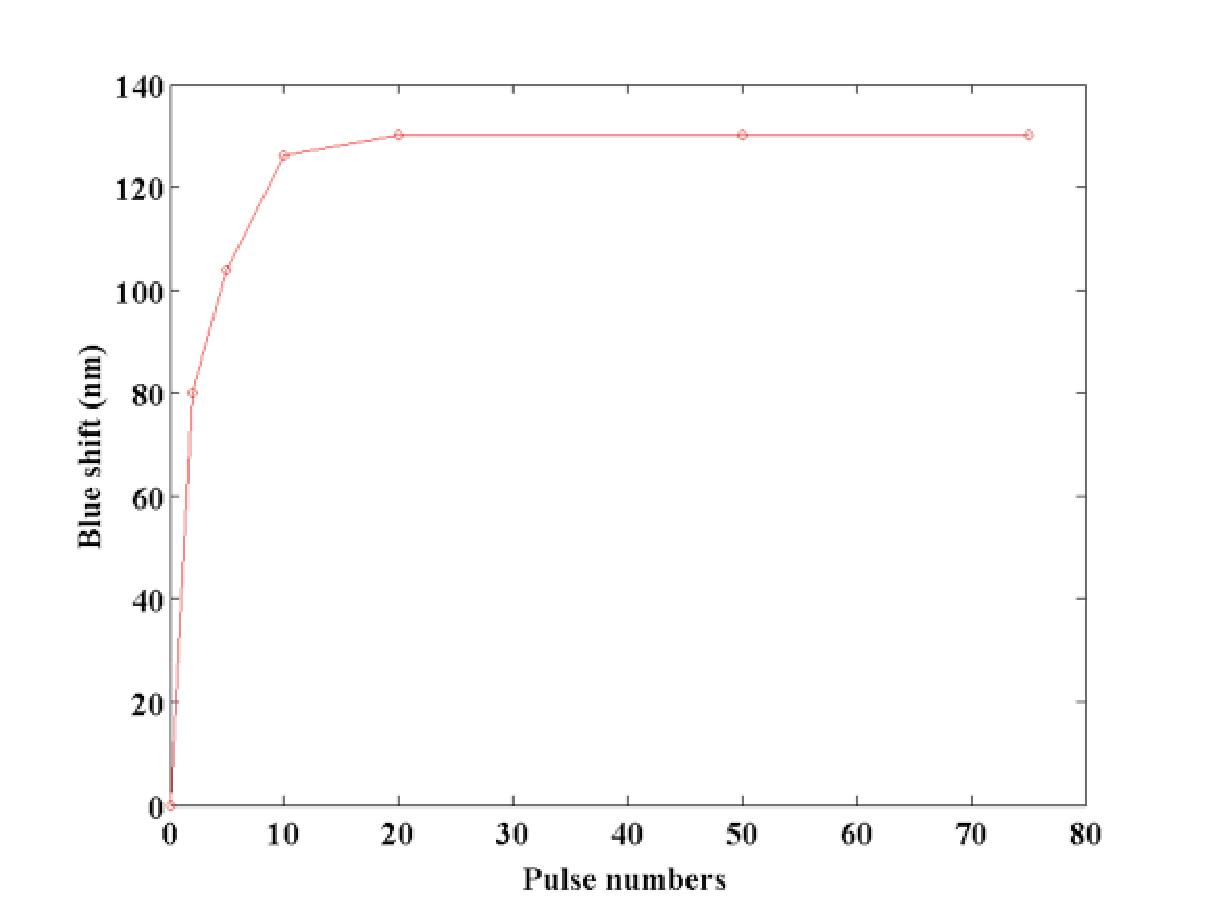
\includegraphics[width=0.7\textwidth]{./Pictures/qwi_pulse.eps}
    \caption{不同脉冲数条件下的蓝移对比}
    \label{fig_qwi_pulse}
\end{figure}

\begin{figure}[htbp]
    \centering
    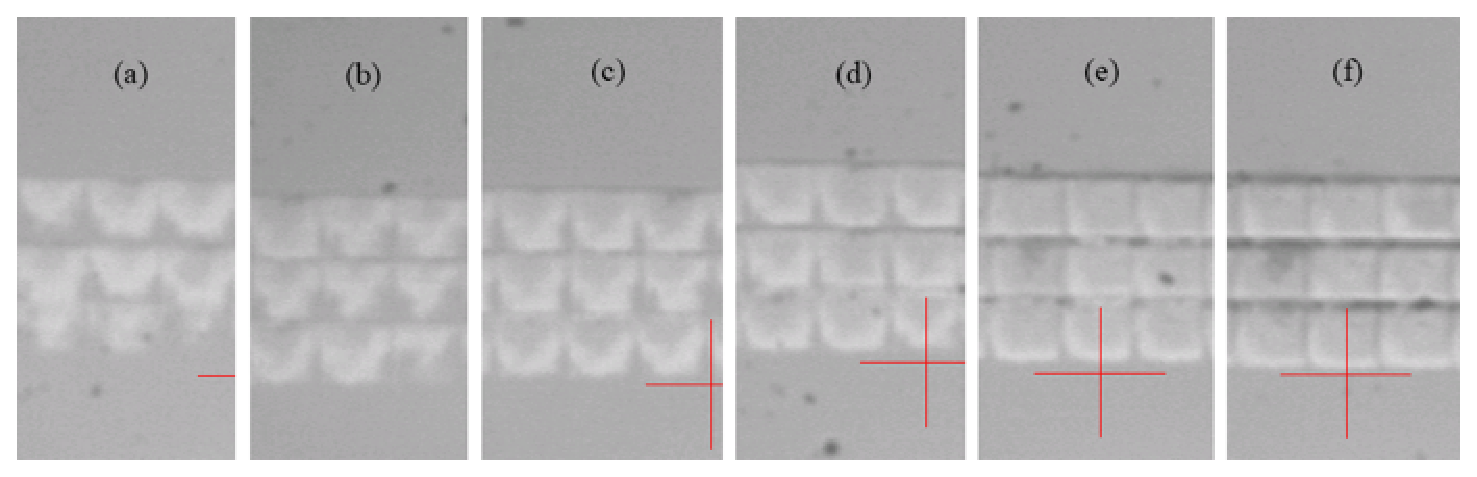
\includegraphics[width=0.7\textwidth]{./Pictures/qwi_pulse2.eps}
    \caption{(a)2脉冲,(b)5脉冲,(c)10脉冲,(d)20脉冲,(e)50脉冲,(f)70脉冲条件下的KrF激光器照射后的图像}
    \label{fig_qwi_pulse2}
\end{figure}

图~\ref{fig_qwi_energy}~是不同能量密度条件下的蓝移对比。当能量密度小于50~mJ/cm2时,PL蓝移随着能量密度的增加而增加。当脉冲数大于50~mJ/cm2时,PL的蓝移稳定在130~nm左右,趋于饱和。由此可见,为了得到较大的蓝移,可以将能量密度稳定在50~mJ/cm2以上。同样,我们还需要考虑照射光斑的均匀性。图~\ref{fig_qwi_energy2}~是不同能量密度条件下的KrF激光器照射后的图像。对于能量密度小于50~mJ/cm2的情况,可以看到每一个小方块图形并不是很完整,主要是因为激光器本身的光斑不够均匀。因此,我们建议使用50~mJ/cm2。

\begin{figure}[htbp]
    \centering
    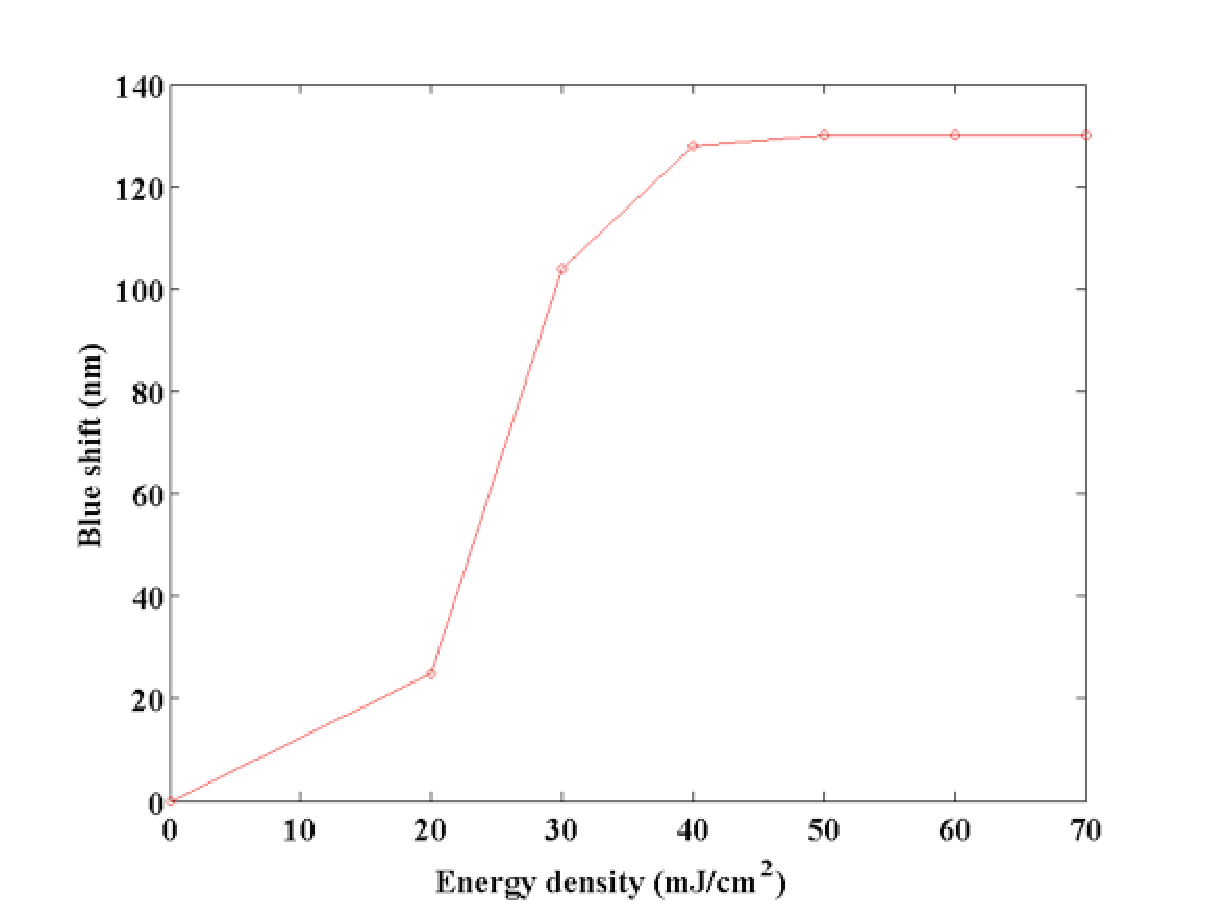
\includegraphics[width=0.7\textwidth]{./Pictures/qwi_energy.eps}
    \caption{不同能量密度条件下的蓝移对比}
    \label{fig_qwi_energy}
\end{figure}

\begin{figure}[htbp]
    \centering
    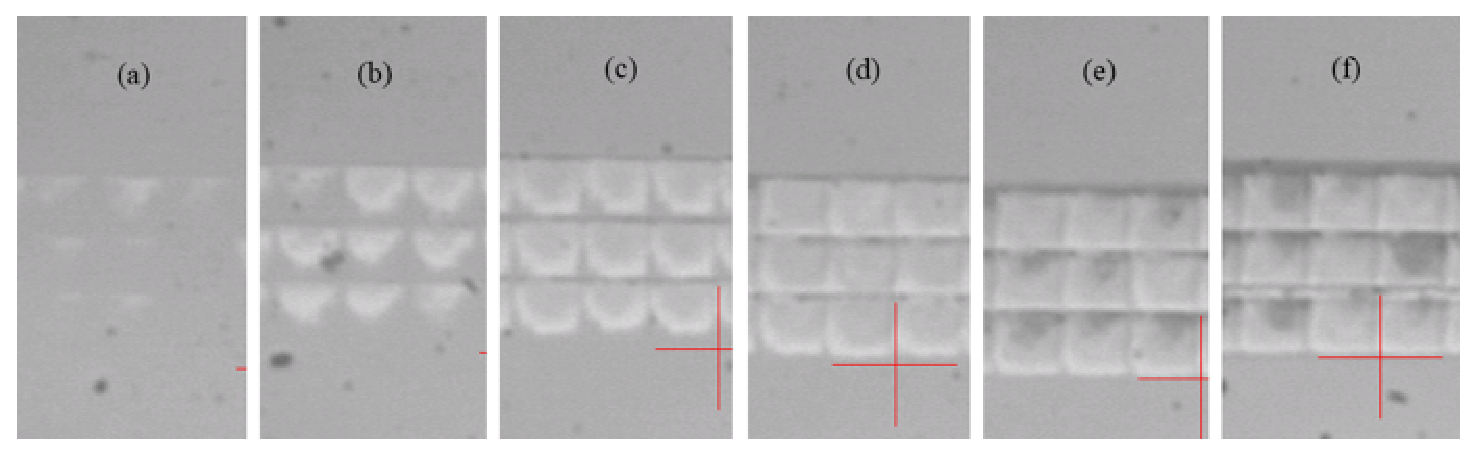
\includegraphics[width=0.7\textwidth]{./Pictures/qwi_energy2.eps}
    \caption{(a)20mJ/cm2,(b)30mJ/cm2,(c)40mJ/cm2,(d)50mJ/cm2,(e)60mJ/cm2,(f)70mJ/cm2条件下的KrF激光器照射后的图像}
    \label{fig_qwi_energy2}
\end{figure}

最后,我们比较不同重复频率条件下的PL蓝移。从图~\ref{fig_qwi_rr}~可以看出,对于重复频率在25~Hz、50~Hz、100~Hz、200~Hz的条件,蓝移都在130~nm左右。所以在这个范围内,取任何的重复频率都是可以的。为了节约加工的时间,我们建议将重复频率尽量取得大一些,如200~Hz。

\begin{figure}[htbp]
    \centering
    \includegraphics[width=0.7\textwidth]{./Pictures/qwi_rr.eps}
    \caption{不同重复频率条件下的蓝移对比}
    \label{fig_qwi_rr}
\end{figure}

综上所述,我们研究了脉冲数、能量密度和重复频率对PL蓝移和混杂区域均匀性的影响。最后我们得到了脉冲数50、能量密度50~mJ/cm2和重复频率200~Hz的优化参数。

%%%%%%%%%%%%%%%%%%%%
\section{利用KrF准分子激光器量子阱混杂制作的简单光器件}
%%%%%%%%%%%%%%%%%%%%

%%%%%%%%%%%%%%%%%%%%
\subsection{FP激光器}
%%%%%%%%%%%%%%%%%%%%

为了探索KrF准分子激光器量子阱混杂技术对InP量子阱芯片的电接触性质的影响,我们制作了一批最简单的FP激光器。首先,取一块1~cm$\times$1~cm大小的InP量子阱片,在其中的一半区域的牺牲层上用KrF准分子激光器扫描。KrF激光器的参数是能量密度50~mJ/cm$^2$,重复频率200~Hz,每个点的脉冲数50,光斑大小40~μm$\times$40~μm。随后芯片被放入快速退火炉中处理,退火温度750$^{\circ}$C,时间90秒。之后,用盐酸溶液腐蚀掉InP牺牲层之后,用激光器的标准工艺步骤制作这些FP激光器。这样制作出来的芯片一半是只做退火的激光器,一半是量子阱混杂后的激光器。激光器的参数是3~μm宽,500~μm长,脊型波导的高度大约1.7~μm。

图~\ref{fig_fp_shift}~是量子阱混杂前后的PL对比图。从图中可以看出,量子阱混杂之后的PL峰值波长在1383~nm左右,而制作退火的区域在1525~nm左右,净蓝移达到了142~nm,这个蓝移量是非常大的。同时,PL的强度在量子阱混杂之后上升了大约34\%,半高全宽为87~nm,相比制作退火区域的90~nm,减少3~nm。这说明量子阱混杂之后,InP量子阱的质量反而变好了。

\begin{figure}[htbp]
    \centering
    \includegraphics[width=0.7\textwidth]{./Pictures/fp_shift.eps}
    \caption{KrF准分子激光器量子阱混杂前后的PL}
    \label{fig_fp_shift}
\end{figure}

在测试FP激光器时,我们首先将激光器放在镀金的氮化铝基片上。基片的下面是带有热敏芯片的半导体制冷片(TEC)。通过调节TEC的温度,控制测试时激光器的温度。下面如果没有特别交代,TEC统一控制在20$^{\circ}$C。激光器的电流由一个直流恒流源通过直流探针直接注入到激光器的电极上。激光器的出射光由一个多模光纤输出到光功率计和光谱仪。图~\ref{fig_fp_li}~是量子阱混杂前后两种FP激光器的L-I特性曲线。从图中可以看出,量子阱混杂之后的FP激光器的阈值电流在28~mA左右,比只做退火的FP激光器的36~mA还要低8~mA。这说明量子阱混杂之后的激光器性能更好,这个结果与量子阱混杂之后的PL变强变窄也是对应的。

\begin{figure}[htbp]
    \centering
    \includegraphics[width=0.7\textwidth]{./Pictures/fp_li.eps}
    \caption{KrF准分子激光器量子阱混杂前后的FP激光器的L-I曲线}
    \label{fig_fp_li}
\end{figure}

图~\ref{fig_fp_iv}~是量子阱混杂前后的FP激光器的I-V特性曲线。从图中可以看出,量子阱混杂之后的FP激光器的开启电压在0.82~V左右,比之前的激光器的0.75~V上升了0.07~V左右。这主要是由于量子阱混杂之后材料的禁带宽度增加造成的。经过计算可以得出,混杂之后材料的禁带宽度与之前的比值约为1.09,这个比值与开启电压的比值几乎是一致的。这说明KrF准分子激光器量子阱混杂方法不会影响InP量子阱材料的电特性。

\begin{figure}[htbp]
    \centering
    \includegraphics[width=0.7\textwidth]{./Pictures/fp_iv.eps}
    \caption{KrF准分子激光器量子阱混杂前后的FP激光器的I-V曲线}
    \label{fig_fp_iv}
\end{figure}

图~\ref{fig_fp_spectra}~是量子阱混杂前后的FP激光器的光谱。从图中可以看出,FP激光器的激射波长从1535~nm蓝移到了1405~nm,净蓝移达到了130~nm,这个结果与PL的结果也是对应的。其中,激光器的波长分别比PL的波长要大10~nm$\sim$20~nm,这是由于电流注入之后升温造成的。光谱在蓝移之后,形状与蓝移之前也是保持一致的,这进一步说明了KrF准分子激光器量子阱混杂技术在得到很大蓝移的同时,不会影响材料的电特性和光特性。

\begin{figure}[htbp]
    \centering
    \includegraphics[width=0.7\textwidth]{./Pictures/fp_spectra.eps}
    \caption{KrF准分子激光器量子阱混杂前后的FP激光器光谱}
    \label{fig_fp_spectra}
\end{figure}

%%%%%%%%%%%%%%%%%%%%
\subsection{无源波导}
%%%%%%%%%%%%%%%%%%%%

为了探索KrF准分子激光器量子阱混杂技术对材料损耗的影响,我们制作了一些量子阱混杂之后的无源直波导。制作的工艺步骤与前面的FP激光器类似,只是在做完标准激光器流片工艺的平坦化之后直接磨片,所以不需要制作电极和欧姆接触,工艺反而更加简单了。波导的尺寸与激光器完全相同。制作完成的无源波导扫描电子显微镜图片如图~\ref{fig_wg}~所示。

\begin{figure}[htbp]
    \centering
    \includegraphics[width=0.7\textwidth]{./Pictures/wg.eps}
    \caption{KrF准分子激光器量子阱混杂制作的无源波导的电镜图片}
    \label{fig_wg}
\end{figure}

然后,我们利用FP干涉法测量波导的损耗。当一个可调谐激光器的光源从波导的一端射入时,由于在波导两端会发生来回多次反射的现象,所以在另一端的出射光谱中可以发现由干涉引起的震荡波纹\cite{Feuchter1994High}。这些波纹的对比度和波导的损耗是正相关的,具体的推导可以参考前人的资料\cite{戴道锌2005阵列波导光栅的理论建模与优化设计及其实验研究}。在测试的时候,我们采用1460~nm$\sim$1620~nm的可调谐激光器作为光源。光经过单模保偏透镜光纤射入波导的一个解理面。由于该波导结构主要在TE模式传输光,TM模式是吸收的,所以需要调整偏正控制器,保证入射光是TE模式的。在波导的另一个解理面,用同样的单模保偏透镜光纤收集出射光,最后由InGaAs光探测器接收。图~\ref{fig_fp_loss}~是量子阱混杂前后的无源波导的透射谱。从图中可以看出,量子阱混杂之后,吸收边界的波长从1560~nm左右移动到了1460~nm左右,所以透射谱蓝移了100~nm以上。接下来我们比较两个透射谱在各自透明区域的损耗。通过计算可以得出,对于只做退火的波导,在1610~nm附近的损耗大约为22~dB/cm。而量子阱混杂的波导,在1550~nm处的损耗为20~dB/cm。这说明量子阱混杂之后,波导的损耗反而略微下降了。所以,KrF准分子激光器量子阱混杂技术不仅不会增加材料的损耗,反而可以略微减小材料的损耗。

\begin{figure}[htbp]
    \centering
    \includegraphics[width=0.7\textwidth]{./Pictures/fp_loss.eps}
    \caption{KrF准分子激光器量子阱混杂前后的无源波导透射谱}
    \label{fig_fp_loss}
\end{figure}

%%%%%%%%%%%%%%%%%%%%%%%%%%%%%%%%%%%%%%%%%%
\chapter{基于量子阱混杂技术的V型腔半导体激光器}
%%%%%%%%%%%%%%%%%%%%%%%%%%%%%%%%%%%%%%%%%%

%%%%%%%%%%%%%%%%%%%%
\section{V型腔可调谐半导体激光器介绍}
%%%%%%%%%%%%%%%%%%%%

V型腔激光器是一种新型的数字式可调谐激光器。与广为人知的SGDBR相比,它不包含光栅结构,而且只需要三个电极进行控制,所以器件更小,结构更简单。它的制作过程与最简单的FP激光器相似,所以制作成本更低。同时,它的波长调谐性能和单模性能也非常好,所以在光通信和光互连方向有非常广阔的应用前景。

V型腔激光器的显微镜图片如图~\ref{fig_vccl}所示。它的结构主要由两个长度不同的FP腔构成。其中一个腔的腔长决定了激光器的波长间隔,这个腔通常被定义为固定增益腔。为了让激光器的波长间隔符合国际电信联盟的100~GHz标准,我们需要将固定腔的腔长定为466.24~μm。另一个腔的长度与固定腔的长度存在微小的差异,这样激光器的波长调谐效果就可以通过游标效应放大,这个腔通常被称为调谐腔。图~\ref{fig_vccl_f}~给出了V型腔激光器的固定腔和调谐腔的谐振频率示意图。其中Δf对应了固定腔的谐振频率间隔,即100~GHz。而Δf’对应了调谐腔的谐振频率间隔。这里假设调谐腔的长度稍微长一些,所以Δf’比Δf稍小。当固定腔和调谐腔的谐振峰在f$_0$处重合时,激光器在f$_0$处的阈值最低,对应了激光的发射波长。同时,谐振峰在f$_1$处会再次发生重合,所以f$_1$-f$_0$=Δf$_c$就是游标效应的自由光谱范围。在这个自由光谱范围之内的波长通道,就是激光器可以调谐得到的所有通道。一般来讲,它必须大于激光器的增益窗口的宽度,避免两个模式同时起振。所以,我们希望腔长差尽量小,这样自由光谱范围就可以尽可能大,调谐得到的通道数就会更多。通过计算可以得到,对于腔长差10\%的情况,一个自由光谱范围可以覆盖约10个通道,对于5\%的情况,通道数可以达到约20个。

\begin{figure}[htbp]
  \centering
  \includegraphics[width=0.5\textwidth]{./Pictures/vccl.eps}\\
  \caption{V型腔激光器的显微镜图片}
  \label{fig_vccl}
\end{figure}

\begin{figure}[htbp]
  \centering
  \includegraphics[width=0.5\textwidth]{./Pictures/vccl_f.eps}\\
  \caption{V型腔激光器的固定腔和调谐腔的谐振频率示意图}
  \label{fig_vccl_f}
\end{figure}

在设计腔长差的时候,除了要考虑自由光谱范围的大小之外,还要考虑对单模特性的影响。图~\ref{fig_vccl_smsr}~表示V型腔激光器的边模抑制比(SMSR)随归一化强度交叉耦合系数χ的变化曲线。其中的χ是由激光器的耦合器结构决定的一个参数,这里我们主要讨论腔长差的影响。从图中可以看到,当腔长差在10\%时,最大的边模抑制比可以达到42~dB左右,而5\%时只有38~dB左右。显然,腔长差越大时,理论上的边模抑制比就越好。这与之前关于自由光谱范围的描述是相反的。所以对腔长差的设计需要在调谐通道数和边模抑制比上折中考虑。

\begin{figure}[htbp]
  \centering
  \includegraphics[width=0.5\textwidth]{./Pictures/vccl_smsr.eps}\\
  \caption{V型腔激光器的边模抑制比随归一化强度交叉耦合系数χ的变化曲线}
  \label{fig_vccl_smsr}
\end{figure}

最后,激光器需要有一个耦合器,用来将两个谐振腔的光合并起来。然而,为了让激光器的边模抑制比尽可能高,耦合器的相位差必须满足一定条件。图~\ref{fig_vccl_thd}~表示在不同的耦合器相位差条件下,V型腔激光器的主模和边模的阈值差随归一化强度交叉耦合系数χ的变化曲线。显然,在相位差180$^{\circ}$的条件下,主模和边模的阈值差可以达到最大值。为了达到这个要求,耦合器的长度、宽度和波导的间隙都需要精心设计,并且这些参数对相位差的大小是十分敏感的。为了排除激光器解理时对耦合器长度的影响,激光器的两端设计了三个刻蚀面,用来准确地控制耦合器和波导的长度。

\begin{figure}[htbp]
  \centering
  \includegraphics[width=0.5\textwidth]{./Pictures/vccl_thd.eps}\\
  \caption{在不同的耦合器相位差条件下,V型腔激光器的主模和边模的阈值差随归一化强度交叉耦合系数χ的变化曲线}
  \label{fig_vccl_thd}
\end{figure}

当激光器工作时,耦合器和固定腔被注入固定的电流提供增益,而调谐腔被注入一个改变的电流,提供增益的同时改变折射率。当调谐腔的电流变化时,调谐腔的材料折射率会发生变化,从而导致整个激光器波长的变化。

自从在2008年被提出以来\cite{He2008Wavelength},V型腔激光器在InP和GaAs材料上都被制作了出来。2011年,金嘉亮等人在InP材料上首次制作出了边模抑制比达到40dB的V型腔激光器\cite{Jin2011Widely}。其中,10\%的激光器可以调谐16个通道,边模抑制比达到了40~dB。5\%的激光器可以调谐26个通道,边模抑制比达到了37~dB。2013年,张森等人制作出了可以覆盖整个C波段的V型腔激光器\cite{Zhang2013Simple}。5\%的激光器可以调谐31个通道,边模抑制比达到了38~dB。通过改变TEC的温度,可以将调谐的通道数增加到50个,从而覆盖了整个C波段的范围。同年,魏文雄等人首次在GaAs材料上制作出了V型腔激光器\cite{Wei2013GaAs}。5\%的激光器可以调谐31个通道,边模抑制比达到了36~dB。2014年,庄园等人制作了利用解理面做为反射面的V型腔激光器,可以连续调谐30个通道,边模抑制比在30~dB以上\cite{Yuan201430}。

然而,以上所有的激光器在调谐的过程中都是基于改变温度的方法,以下简称热调谐。当激光器调谐腔注入的电流增大时,该谐振腔的温度上升,折射率上升,导致波长往长波方向移动。这种调谐的方式存在调谐电流大(>100~mA),波长切换时间长(~20~μs)等缺点。改进的方法是使用基于载流子注入的方法,以下简称电调谐\cite{Shim1995Refractive}。理论上,使用电调谐时,调谐电流可以大大减小,同时波长切换时间可以缩短到纳秒量级\cite{Guo2012Experimental}。为了达到这个效果,V型腔激光器的调谐腔需要处理成无源的谐振腔,这就需要用到量子阱混杂技术。

图~\ref{fig_vccl_qwi_strategies}~表示了基于电调谐的V型腔激光器的两个方案。第一个方案是将一个调谐腔电极覆盖的波导处理成无源波导。当激光器工作时,耦合器和固定腔注入固定的电流提供增益,调谐腔注入变化的电流改变折射率。假设调谐腔是较短的那个腔,当调谐腔的电流增加时,随着载流子浓度的增加,调谐腔的折射率随之减小,激光器的波长会往长波方向移动。第二个方案是将调谐腔电极和固定腔电极覆盖的波导同时处理成无源波导。当激光器工作时,耦合器注入固定的电流提供增益,固定腔电极不需要注入电流,调谐腔注入变化的电流改变折射率。假设调谐腔是较长的那个腔,当调谐腔的电流增加时,随着载流子浓度的增加,调谐腔的折射率随之减小,激光器的波长会往短波方向移动。在后面的测试结果与分析中,这两种方案都会被讨论。

\begin{figure}[htbp]
  \centering
  \includegraphics[width=0.7\textwidth]{./Pictures/vccl_qwi_strategies.eps}\\
  \caption{单腔混杂(a)和双腔混杂(b)方案的V型腔激光器示意图}
  \label{fig_vccl_qwi_strategies}
\end{figure}

除此之外,量子阱混杂波导的长度占整个波导长度的比例也是一个重要的参数。在以往的V型腔激光器中,调谐腔电极覆盖的波导长度与耦合器电极覆盖波导的长度比例通常固定为4:6,这个参数对激光器性能的影响并没有深入研究。本文中我们将采用2:8和4:6两种方案进行研究。

%%%%%%%%%%%%%%%%%%%%
\section{包含量子阱混杂的V型腔激光器的制作过程}
%%%%%%%%%%%%%%%%%%%%

包含量子阱混杂的V型腔激光器的制作过程主要包含三个步骤:制作对准标记,选择性区域量子阱混杂以及全有源V型腔的标准制作流程。由于两种量子阱混杂V型腔激光器方案的制作过程完全相同,这里只给出一个腔量子阱混杂方案的大致工艺过程。

%%%%%%%%%%%%%%%%%%%%
\subsection{制作对准标记}
%%%%%%%%%%%%%%%%%%%%

由于量子阱混杂处理完之后的量子阱片表面是看不到任何痕迹的,后面的图形无法直接与其对准,所以必须在整个制作流程的一开始制作对准标记。这样一来,量子阱混杂的图形和后面的图形都与这层对准标记对准,也就实现了混杂图形和后面图形的相互对准。图~\ref{fig_marker}~是对准标记掩膜板的CAD截图。制作的流程主要采用了标准的光刻和干法刻蚀的工艺流程,具体步骤如表~\ref{marker}~所示。

\begin{figure}[htbp]
  \centering
  \includegraphics[width=0.5\textwidth]{./Pictures/marker.eps}\\
  \caption{对准标记掩膜板的CAD截图}
  \label{fig_marker}
\end{figure}

\begin{table}[htbp]
    \zihao{5}
    \caption{对准标记工艺流程}
    \centering
    \label{marker}
    \begin{tabular}{ccc}
        \hline
        \hline
        流程 & 细节 & 备注\\
        \hline
        光刻 &旋涂AZ5214 &\\
            &烘烤90$^{\circ}$C 6分钟 &\\
            &曝光 & 反转光刻胶\\
            &烘烤120$^{\circ}$C 2分钟 &\\
            &空曝 2分钟 &\\
            &显影45秒 &\\
        \hline
        刻蚀二氧化硅 &ICP刻蚀二氧化硅 4分钟 &\\
            &ICP氧清洗 5分钟 & 去除光刻胶\\
        \hline
        刻蚀InP &ICP刻蚀InP 2分钟 &刻穿牺牲层\\
            &BOE腐蚀5分钟 &去除二氧化硅\\
        \hline
        \hline
    \end{tabular}
\end{table}

%%%%%%%%%%%%%%%%%%%%
\subsection{选择性区域量子阱混杂}
%%%%%%%%%%%%%%%%%%%%

详细的工艺流程如表~\ref{qwi_regions}~所示。其中真正的量子阱混杂步骤从KrF准分子激光器照射开始,之前的步骤是用来制作识别混杂区域的二氧化硅窗口的。图~\ref{fig_windows}~是量子阱混杂窗口掩膜板的CAD截图。其中的窗口尺寸在40~μm$\times$200~μm左右,当然两个腔混杂的方案中,窗口会更大一些。在量子阱混杂开始之前,一系列这样的二氧化硅窗口会在牺牲层表面制作出来,其中窗口的外面是200~nm厚的二氧化硅,里面没有二氧化硅。这些二氧化硅虽然不能反射KrF激光,但是可以通过这些图形识别哪些区域需要进行混杂。在这些窗口制作好之后,40~μm$\times$40~μm尺寸的KrF准分子激光光束会在每一个窗口中进行手动扫描,保证窗口中的每一个地方都能扫到。KrF准分子激光器的能量密度为50~mJ/cm2,重复频率为200~Hz,脉冲数为50。在KrF准分子激光器照射之后,样品被放入快速退火炉中退火,条件是750$^{\circ}$C 90秒。在退火的过程中,样品被夹在两块新的硅片中间。最后,去掉表面的二氧化硅层和InP牺牲层,量子阱混杂的步骤就全部完成了。这里需要指出的是,某些条件下生长的二氧化硅在快速退火的条件下会引起量子阱混杂。混杂的条件是二氧化硅的下面一层材料中含有镓元素,而且退火温度要足够高(800$^{\circ}$C左右)。这里的二氧化硅生长在InP牺牲层上面,所以不会引起量子阱混杂。如果在快速退火之前去掉二氧化硅也是可以的。

\begin{figure}[htbp]
  \centering
  \includegraphics[width=0.5\textwidth]{./Pictures/windows.eps}\\
  \caption{量子阱混杂窗口掩膜板的CAD截图}
  \label{fig_windows}
\end{figure}

\begin{table}[htbp]
    \zihao{5}
    \caption{选择性区域量子阱混杂工艺流程}
    \centering
    \label{qwi_regions}
    \begin{tabular}{ccc}
        \hline
        \hline
        流程 & 细节 & 备注\\
        \hline
        长膜 &PECVD生长二氧化硅200nm &\\
        \hline
        光刻 &旋涂AZ5214 &\\
            &烘烤90$^{\circ}$C 6分钟 &\\
            &曝光 & 反转光刻胶\\
            &烘烤120$^{\circ}$C 2分钟 &\\
            &空曝 2分钟 &\\
            &显影45秒 &\\
        \hline
        刻蚀二氧化硅 &ICP刻蚀二氧化硅 4分钟 &\\
            &ICP氧清洗 5分钟 & 去除光刻胶\\
        \hline
        量子阱混杂 &KrF准分子激光器照射 50~mJ/cm$^2$ 50~Hz 50脉冲 &\\
            &快速热退火 750$^{\circ}$C 90秒 &\\
        \hline
        后续处理 &去除二氧化硅 &\\
            &去除牺牲层 &\\
        \hline
        \hline
    \end{tabular}
\end{table}

%%%%%%%%%%%%%%%%%%%%
\subsection{V型腔激光器的标准制作流程}
%%%%%%%%%%%%%%%%%%%%

由于全有源的V型腔激光器在前人的论文中已经提及过\cite{金嘉亮2012基},这里不再详细讨论。表\ref{vccl_fab}列出了大致的工艺流程,仅供参考。

\begin{table}[htbp]
    \zihao{6}
    \caption{全有源V型腔激光器的标准制作流程}
    \centering
    \label{vccl_fab}
    \begin{tabular}{ccc}
        \hline
        \hline
        流程 & 细节 & 备注\\
        \hline
        长膜 &PECVD生长二氧化硅1000nm &制作刻蚀面开始\\
        \hline
        光刻 &旋涂AZ5214 &\\
            &烘烤90$^{\circ}$C 6分钟 &\\
            &曝光 &\\
            &显影45秒 &\\
        \hline
        刻蚀二氧化硅 &ICP刻蚀二氧化硅 9分钟 &\\
            &ICP氧清洗 5分钟 & 去除光刻胶\\
            &显影液浸泡 30分钟 &去除氟碳化合物\\
        \hline
        刻蚀InP &InGaAs腐蚀45秒 \\
            &ICP刻蚀InP 4分钟 &\\
            &BOE腐蚀5分钟 &去除二氧化硅\\
        \hline
        长膜 &PECVD生长二氧化硅500nm &制作波导开始\\
        \hline
        光刻 &旋涂AZ5214 &\\
            &烘烤90$^{\circ}$C 6分钟 &\\
            &曝光 &\\
            &显影45秒 &\\
        \hline
        刻蚀二氧化硅 &ICP刻蚀二氧化硅 4分钟 &\\
            &ICP氧清洗 5分钟 & 去除光刻胶\\
            &显影液浸泡 30分钟 &去除氟碳化合物\\
        \hline
        刻蚀InP &ICP刻蚀InP 1分40秒 &\\
            &盐酸溶液腐蚀3秒 &\\
            &BOE腐蚀5分钟 &去除二氧化硅\\
        \hline
        平坦化 &旋涂BCB &\\
            &烘烤260$^{\circ}$C 1小时 &\\
            &ICP刻蚀BCB 1分钟 &\\
        \hline
        光刻 &旋涂AZ5214 &制作电极开始\\
            &烘烤90$^{\circ}$C 6分钟 &\\
            &曝光 & 反转光刻胶\\
            &烘烤120$^{\circ}$C 2分钟 &\\
            &空曝 2分钟 &\\
            &显影 45秒 &\\
        \hline
        溅射 &溅射Ti Pt Au &\\
        \hline
        剥离 &丙酮超声波5分钟 &\\
        \hline
        电隔离 &ICP刻蚀InP 25秒 &\\
        \hline
        去除刻蚀面BCB &ICP刻蚀BCB15分钟 &\\
        \hline
        磨片 &厚度减到200微米之内再抛光 &\\
        \hline
        溅射 &背面溅射Ti Pt Au &\\
        \hline
        欧姆接触 &快速退火480$^{\circ}$C 1分钟 &\\
        \hline
        \hline
    \end{tabular}
\end{table}

%%%%%%%%%%%%%%%%%%%%
\section{单腔混杂方案的测试结果与分析}
%%%%%%%%%%%%%%%%%%%%

%%%%%%%%%%%%%%%%%%%%
\subsection{光致发光谱}
%%%%%%%%%%%%%%%%%%%%

这里为了得到整个芯片PL的二维空间分布,我们将样品放在电动二维平移台上(Suruga seiki D212 motorized stage controller),并用电脑由GPIB协议控制其移动。每移动一个点,就由PL测试装置测得这个点的PL峰值波长和强度。这个系统有两点需要注意的地方。首先,扫描整个芯片的时间可能会很长。假设每个点收集PL数据需要一秒钟时间,对于1~cm$\times$1~cm大小的芯片,扫描100$\times$100个点,即步长100~μm,忽略移动的时间,总共需要的时间为10000秒=2.8小时。100~μm的步长已经相当长了,通常的量子阱混杂窗口尺度在几十个微米,所以很难一次性扫描整个芯片得到细节,只能粗扫整片,细扫局部。同时每个点的扫描时间主要由光谱仪的span、RBW (resolution bandwidth) 和reference level决定。需要尽量把span减小,RBW和reference level提高。另一个问题是测试的空间分辨率。虽然D212的移动步长最小可以达到1μm,但是分辨率也受制于PL测试装置的入射光斑尺寸。由于1064nm激发光源是通过多模光纤垂直入射到芯片表面的,所以光斑尺寸和多模光纤的芯径差不多,在几十个微米到几百微米之间。所以当测量的量子阱混杂图形尺寸在40μm左右时,入射光斑中只有一部分光用来激发混杂之后的PL,另一部分光激发相邻的混杂之前芯片的PL,这样测得的强度可能小于实际的PL值。当一小部分光斑位于量子阱混杂图形上,大部分在外面时,PL的峰值波长还是混杂区域之外的PL波长,但是强度已经开始下降了;当这两部分光斑的尺寸相同时,正好处于临界值,两个PL同时出现,强度大约是一半一半;当大部分光斑位于量子阱混杂图形上时,测试得到的PL峰值波长才是混杂之后的PL的峰值波长。

图~\ref{fig_single_pl}~是一个量子阱混杂窗口的PL二维扫描图。窗口的尺寸是40~μm$\times$200~μm。从波长图中可以看出,量子阱混杂窗口内的波长在1400~nm到1410~nm之间,窗口外的波长在1500~nm左右,所以净蓝移在90~nm到100~nm之间。从强度图中可以看出,窗口内的强度大约是外面的40\%,接近一半。根据上面对PL系统的分析,由于窗口在宽度尺寸上很小,强度的值可能是不准确的,最大的差距在一半左右。这里的测试结果与上面的分析是吻合的。

\begin{figure}[htbp]
  \centering
  \includegraphics[width=1.0\textwidth]{./Pictures/single_pl.eps}\\
  \caption{PL波长(a)和PL强度(b)}
  \label{fig_single_pl}
\end{figure}

图~\ref{fig_single_pl2}~是量子阱混杂窗口内和窗口外两个点的PL谱。从图中可以看出,蓝移前后的PL峰值波长分别为1505~nm和1410~nm,所以净蓝移95~nm。同时蓝移后强度下降到之前的43\%。

\begin{figure}[htbp]
  \centering
  \includegraphics[width=0.7\textwidth]{./Pictures/single_pl2.eps}\\
  \caption{快速热退火和量子阱混杂区域的PL谱}
  \label{fig_single_pl2}
\end{figure}

%%%%%%%%%%%%%%%%%%%%
\subsection{I-V性能}
%%%%%%%%%%%%%%%%%%%%

图~\ref{fig_single_iv}~给出了耦合器、调谐腔和固定腔的I-V特性曲线。由于这三个腔的波导的形状和尺寸完全不同,所以曲线在电流加大之后的规律不太一样,但是这三条曲线的趋势都是正常的二极管I-V趋势。这里我们主要关注开启电压。对于耦合器和固定腔,开启电压在0.8~V左右,而量子阱混杂之后的调谐腔的开启电压略大,在0.85~V$\sim$0.9~V左右。这与之前的FP波导的现象是相同的,即混杂之后禁带宽度变大造成的,而且开启电压与禁带宽度基本成正比。这些结果说明,量子阱混杂不会影响V型腔激光器的电接触特性。

\begin{figure}[htbp]
  \centering
  \includegraphics[width=0.7\textwidth]{./Pictures/single_iv.eps}\\
  \caption{耦合器、调谐腔和固定腔的I-V曲线}
  \label{fig_single_iv}
\end{figure}

%%%%%%%%%%%%%%%%%%%%
\subsection{波长调谐性能}
%%%%%%%%%%%%%%%%%%%%

最后我们研究该激光器的波长调谐性能。由于量子阱混杂区域是V型腔激光器的短腔,所以这个腔作为调谐腔。耦合器和长腔都是有源量子阱材料,所以需要加固定的电流提供增益。在实际的测试中,耦合器和长腔的电流分别为60~mA和30~mA,事实上这两个电流的大小并不会对波长调谐性能产生影响,只要提供足够的增益就可以了。图~\ref{fig_single_tuning_p10}~是10\%腔长差激光器的波长与调谐电流的变化关系。当调谐电流为0时,激光器波长为1512~nm左右,这与前面的量子阱混杂窗口外面的PL峰值波长1505~nm是对应的。由于注入电流产生的热效应,一般激光器的波长会比PL波长要长10~nm左右。当调谐腔的电流增加时,随着载流子浓度的增加,调谐腔的折射率随之减小,激光器的波长会往长波方向移动,所以图中的波长从1512.2~nm逐步变化到1517.6~nm,一共9个通道。其中有个别通道会随着电流变化产生一个很小的跳变,这是由于光谱仪的精度0.08~nm造成的。当进一步增加电流时,波长会从1517.6~nm直接调回1512.2~nm左右,即跳回这个FSR的开始。理论上,10\%腔长差的V型腔激光器的FSR包含10个左右的通道,所以这里的结果与理论上也是符合的。此外,波长变化的趋势是,随着电流的增加,单位电流带来的波长变化效果是逐渐减小的。这是由于载流子注入的效果是非线性的,同时电流增加带来温度变化导致的波长变化会往反方向运动,这样就造成了载流子注入效果逐渐减弱,导致非线性的调谐结果。值得一提的是,调谐电流最大只有25~mA,比热调谐的电流要小得多。

\begin{figure}[htbp]
  \centering
  \includegraphics[width=0.7\textwidth]{./Pictures/single_tuning_p10.eps}\\
  \caption{波长调谐曲线(10\%腔长差)}
  \label{fig_single_tuning_p10}
\end{figure}

图~\ref{fig_single_spectra_p10}是该激光器调谐得到的9个通道叠加的光谱。从图中可以看出,每个通道的边模抑制比都在30~dB以上,其中最好的一个如图~\ref{fig_single_spectrum_p10}~所示可以到达34dB。这个结果还算可以接受,但是与以往的10\%热调谐V型腔激光器相比,过去的结果最好可以达到40~dB,仍然有至少6~dB的差距。这个差距的原因是多方面的,但是最主要的原因是单腔混杂本身的原因。在V型腔激光器中,要达到最佳的边模抑制比,需要满足等回路增益条件。也就是固定腔和调谐腔的增益要尽可能的完全对称。在单腔混杂的方案中,由于固定腔是有源腔,尽管所加的电流不大,也能提供一部分增益,而调谐腔可以视为完全无源的腔,所以理论上要达到等回路增益条件还需要优化激光器本身的其他参数。此外,制作工艺本身也是重要的因素。这一批激光器的设计与之前的热调谐V型腔激光器的设计完全相同,只是多加了一步量子阱混杂的工艺,所以用了同一块掩膜板。这块掩膜板使用的时间比较长,线条清晰度已经大不如前,这样就给激光器的制作质量带来了影响。

\begin{figure}[htbp]
  \centering
  \includegraphics[width=0.7\textwidth]{./Pictures/single_spectra_p10.eps}\\
  \caption{9个通道叠加的光谱(10\%腔长差)}
  \label{fig_single_spectra_p10}
\end{figure}

\begin{figure}[htbp]
  \centering
  \includegraphics[width=0.7\textwidth]{./Pictures/single_spectrum_p10.eps}\\
  \caption{单个通道的光谱(10\%腔长差)}
  \label{fig_single_spectrum_p10}
\end{figure}

5\%腔长差的波长调谐结果如图~\ref{fig_single_tuning_p5}~所示。当调谐电流为0时,激光器波长为1513~nm左右,这与前面的量子阱混杂窗口外面的PL峰值波长1505~nm是对应的。由于注入电流产生的热效应,一般激光器的波长会比PL波长要长10~nm左右。当调谐腔的电流增加时,随着载流子浓度的增加,调谐腔的折射率随之减小,激光器的波长会往长波方向移动,所以图中的波长从1513.2~nm逐步变化到1524.4~nm,一共18个通道。当进一步增加电流时,波长会从1524.4~nm直接调回1513.2~nm左右,即跳回这个FSR的开始。理论上,5\%腔长差的V型腔激光器的FSR包含20个左右的通道,所以这里的结果与理论上也是符合的。另外,调谐电流在12~mA以下,比热调谐的电流小一个数量级。

\begin{figure}[htbp]
  \centering
  \includegraphics[width=0.7\textwidth]{./Pictures/single_tuning_p5.eps}\\
  \caption{波长调谐曲线(5\%腔长差)}
  \label{fig_single_tuning_p5}
\end{figure}

图~\ref{fig_single_spectra_p5}是该激光器调谐得到的18个通道叠加的光谱。从图中可以看出,每个通道的边模抑制比都在30~dB左右,其中最好的一个如图~\ref{fig_single_spectrum_p5}~所示可以到达32~dB。这个结果还算可以接受,但是和上面10\%腔长差的结果类似,与以往的5\%热调谐V型腔激光器相比,过去的结果最好可以达到37~dB,仍然有大约5~dB的差距。

\begin{figure}[htbp]
  \centering
  \includegraphics[width=0.7\textwidth]{./Pictures/single_spectra_p5.eps}\\
  \caption{18个通道叠加的光谱(5\%腔长差)}
  \label{fig_single_spectra_p5}
\end{figure}

\begin{figure}[htbp]
  \centering
  \includegraphics[width=0.7\textwidth]{./Pictures/single_spectrum_p5.eps}\\
  \caption{单个通道的光谱(5\%腔长差)}
  \label{fig_single_spectrum_p5}
\end{figure}

总的来说,我们成功地将KrF准分子激光器量子阱混杂技术应用到单腔混杂的V型腔激光器中,实现了覆盖一整个FSR范围的电调谐的效果。对于10\%腔长差来说,波长调谐范围是9个通道,边模抑制比34~dB,调谐电流在25~mA以下。对于5\%腔长差来说,波长调谐范围是18个通道,边模抑制比32~dB,调谐电流在12~mA以下。其中的调谐范围和理论完全符合,说明利用该量子阱混杂技术实现电调谐是很成功的。另一方面,边模抑制比比以往的热调谐V型腔激光器要差5~dB,主要是由单腔混杂的结构和工艺流程的缺陷造成的。

%%%%%%%%%%%%%%%%%%%%
\section{双腔混杂方案的测试结果与分析}
%%%%%%%%%%%%%%%%%%%%

%%%%%%%%%%%%%%%%%%%%
\subsection{光致发光谱}
%%%%%%%%%%%%%%%%%%%%

对于双腔混杂的V型腔激光器,我们在量子阱混杂的掩膜设计上进行了改进。这一次我们将两个无源腔的量子阱混杂区域合在一起,形成一个200~μm$\times$200~μm的更大的矩形窗口。这个尺寸大于PL系统的入射光斑,就可以准确测得PL的强度。图~\ref{fig_double_pl}是整一块芯片的PL二维图。其中的每个量子阱混杂窗口在100×100的扫描格点中都可以看到。窗口之内的波长在1425~nm左右,外面的波长在1530~nm左右,所以净蓝移在105~nm左右。而且整一块芯片的未量子阱混杂区域和混杂区域各自的波长非常都均匀,说明该方法的均匀性非常好。芯片的右下角有大约1/8的区域没有做量子阱混杂处理,这些是没有混杂的激光器区域,用来和混杂之后的激光器做对比。右边的图中大部分窗口的强度似乎是下降的,这主要是由于扫描的步长太大了。更准确的信息可以从图~\ref{fig_double_pl2}~中得到。该图缩小了扫描范围,仅包含了9个窗口。这一次可以从强度图中看到每一个窗口的中心位置的强度,与窗口外面的强度相比不仅没有下降,反而是略微上升的。

\begin{figure}[htbp]
  \centering
  \includegraphics[width=1.0\textwidth]{./Pictures/double_pl.eps}\\
  \caption{PL波长二维图(a)和PL强度二维图(b)}
  \label{fig_double_pl}
\end{figure}

\begin{figure}[htbp]
  \centering
  \includegraphics[width=1.0\textwidth]{./Pictures/double_pl2.eps}\\
  \caption{PL波长二维图(a)和PL强度二维图(b)}
  \label{fig_double_pl2}
\end{figure}

为了更细致地得到每一个窗口的PL信息,图~\ref{fig_double_pl3}~给出了单个量子阱混杂窗口的PL二维图。从波长图中可以看到,量子阱混杂之后的波长从1530~nm蓝移到1425~nm左右,净蓝移105~nm,这与上面的信息是吻合的。而且,在蓝移和为蓝移两个区域的边界的地方,波长是瞬间跳变的,这说明这种量子阱混杂的方法有非常好的空间分辨率。而在PL强度图中,可以观察到边界的地方有一个明显的圈,在这个圈上的强度会下降到外面的一半,这是由于PL测试光斑一半用来激发窗口外的PL,一半用于激发窗口内的PL,所以两种PL同时存在,强度正好一半一半。这与前面的描述也是相同的。在这个圈的内部,PL的强度不仅没有比外面的低,而且比外面还要高。这说明经过这种量子阱混杂技术处理之后的芯片,不仅质量不会变差,反而变得更好了。这与前面FP激光器的阈值和无源波导的损耗结果是一致的。

\begin{figure}[htbp]
  \centering
  \includegraphics[width=1.0\textwidth]{./Pictures/double_pl3.eps}\\
  \caption{PL波长二维图(a)和PL强度二维图(b)}
  \label{fig_double_pl3}
\end{figure}

在量子阱混杂窗口里面和外面的两点的PL对比图如图~\ref{fig_double_pl4}~所示。从图中可以看到,量子阱混杂之后,PL峰值波长从1530~nm移动到1425~nm,净蓝移105~nm,同时强度上升了约20\%。这个结果是比较理想的。图中1375~nm处的PL存在一个小峰,经验证这不是由量子阱造成的,不会影响后面制作激光器的结果。

\begin{figure}[htbp]
  \centering
  \includegraphics[width=0.7\textwidth]{./Pictures/double_pl4.eps}\\
  \caption{快速热退火和量子阱混杂区域的PL谱}
  \label{fig_double_pl4}
\end{figure}

%%%%%%%%%%%%%%%%%%%%
\subsection{L-I性能}
%%%%%%%%%%%%%%%%%%%%

图~\ref{fig_double_li}~给出了双腔混杂和全有源V型腔激光器的L-I特性曲线图。由于双腔混杂V型腔激光器只有耦合器部分是有源材料,其他两个腔已经处理成无源材料,所以只需要在耦合器上加电就可以产生激光,另两个腔加电之与否理论上对增益并没有什么影响。所以这里固定腔和调谐腔不加电。对于全有源V型腔激光器来说,在掩膜板中已经设计成三个电极连在一起,所以只有一个电极。从图中可以看出,两种激光器的阈值电流都在50~mA$\sim$60~mA之间,微分增益几乎是相同的。这说明两种激光器在L-I性能上是基本差不多的。本质上来说,这里的双腔混杂激光器就是一个延长器激光器,它的阈值电流由有源波导和无源波导长度的比例决定。这里要理论上比较上述两种激光器的阈值是比较复杂的,这里我们不做深入探讨,只要得出两种激光器L-I性能相似的结果就可以了。

\begin{figure}[htbp]
  \centering
  \includegraphics[width=0.7\textwidth]{./Pictures/double_li.eps}\\
  \caption{全有源和双腔混杂的V型腔激光器的L-I曲线}
  \label{fig_double_li}
\end{figure}

%%%%%%%%%%%%%%%%%%%%
\subsection{单电极波长调谐性能}
%%%%%%%%%%%%%%%%%%%%

双腔混杂V型腔激光器的波长调谐性能与单腔混杂的情况有所不同。不同的地方在于,由于固定腔和调谐腔都被处理成无源波导,所以只需要改变一个腔的电流,另一个腔不需要加电。而且电流加在任意一个腔上都可以,只是调谐的方向相反而已。理论上,调谐的范围和腔长成正比,所以这里我们只对长腔加电流,作为调谐腔,而短腔作为固定腔,不加电流。图~\ref{fig_double_tuning_p10}~是10\%腔长差的波长与调谐电流的变化关系。当调谐电流为0时,激光器波长为1531.6~nm左右,这与前面的量子阱混杂窗口外面的PL峰值波长1530~nm是对应的。当调谐腔的电流增加时,随着载流子浓度的增加,调谐腔的折射率随之减小,激光器的波长会往短波方向移动,所以图中的波长从1531.6~nm逐步变化到1526.4~nm,一共8个通道。其中有个别通道会随着电流变化产生一个很小的跳变,这是由于光谱仪的精度0.08~nm造成的。当进一步增加电流时,波长会从1526.4~nm直接调回1531.6~nm左右,即跳回这个FSR的开始。理论上,10\%腔长差的V型腔激光器的FSR包含10个左右的通道,所以这里的结果与理论上也是基本符合的。另外,调谐电流最大仅17~mA,比热调谐的电流小一个数量级。

\begin{figure}[htbp]
  \centering
  \includegraphics[width=0.7\textwidth]{./Pictures/double_tuning_p10.eps}\\
  \caption{波长调谐曲线(10\%腔长差)}
  \label{fig_double_tuning_p10}
\end{figure}

图~\ref{fig_double_spectra_p10}是该激光器调谐得到的9个通道叠加的光谱。从图中可以看出,每个通道的边模抑制比都在40~dB左右,其中的一个40~dB光谱如图~\ref{fig_double_spectrum_p10}~所示。这个结果与以往的10\%热调谐V型腔激光器相比是一致的。这说明使用KrF准分子激光器量子阱混杂技术制作的双腔混杂V型腔激光器,性能和没有混杂的热调谐V型腔激光器是可以媲美的。

\begin{figure}[htbp]
  \centering
  \includegraphics[width=0.7\textwidth]{./Pictures/double_spectra_p10.eps}\\
  \caption{8通道叠加的光谱(10\%腔长差)}
  \label{fig_double_spectra_p10}
\end{figure}

\begin{figure}[htbp]
  \centering
  \includegraphics[width=0.7\textwidth]{./Pictures/double_spectrum_p10.eps}\\
  \caption{单个通道的光谱(10\%腔长差)}
  \label{fig_double_spectrum_p10}
\end{figure}

图~\ref{fig_double_tuning_p5}~是5\%腔长差的波长与调谐电流的变化关系。当调谐电流为0时,激光器波长为1523~nm左右。当调谐腔的电流增加时,随着载流子浓度的增加,调谐腔的折射率随之减小,激光器的波长会往短波方向移动,所以图中的波长从1523~nm逐步变化到1508.5~nm,一共21个通道。当进一步增加电流时,波长会从1508.5~nm直接调回1523~nm左右,即跳回这个FSR的开始。理论上,5\%腔长差的V型腔激光器的FSR包含20个左右的通道,所以这里的结果与理论上也是符合的。另外,调谐电流最大仅8~mA,比热调谐的电流至少小一个数量级。

\begin{figure}[htbp]
  \centering
  \includegraphics[width=0.7\textwidth]{./Pictures/double_tuning_p5.eps}\\
  \caption{波长调谐曲线(5\%腔长差)}
  \label{fig_double_tuning_p5}
\end{figure}

图~\ref{fig_double_spectra_p5}是该激光器调谐得到的21个通道叠加的光谱。从图中可以看出,每个通道的边模抑制比都在35~dB以上,其中的一个37~dB光谱如图~\ref{fig_double_spectrum_p5}~所示。这个结果与以往的5\%热调谐V型腔激光器相比是基本一致的。这同样说明使用KrF准分子激光器量子阱混杂技术制作的双腔混杂V型腔激光器,性能和没有混杂的热调谐V型腔激光器是可以媲美的。

\begin{figure}[htbp]
  \centering
  \includegraphics[width=0.7\textwidth]{./Pictures/double_spectra_p5.eps}\\
  \caption{21通道叠加的光谱(5\%腔长差)}
  \label{fig_double_spectra_p5}
\end{figure}

\begin{figure}[htbp]
  \centering
  \includegraphics[width=0.7\textwidth]{./Pictures/double_spectrum_p5.eps}\\
  \caption{单个通道的光谱(5\%腔长差)}
  \label{fig_double_spectrum_p5}
\end{figure}

然而,对于一部分5\%腔长差的激光器,调谐性能出现了一些超出上面理论极限的效果。如图~\ref{fig_double_tuning_32ch}~是另一个5\%腔长差激光器的波长与调谐电流的变化关系。当调谐电流为0时,激光器波长为1535~nm左右,这与前面的量子阱混杂窗口外面的PL峰值波长1530~nm是对应的。当调谐腔的电流增加时,随着载流子浓度的增加,调谐腔的折射率随之减小,激光器的波长会往短波方向移动,所以图中的波长从1535~nm逐步变化到1512~nm,一共32个通道。当进一步增加电流时,波长往短波方向的运动趋于饱和,反而向长波方向运动。这是由于当电流增大到40mA时,注入调谐腔的载流子趋于饱和,所以由增加电流产生的热效应开始占主导地位。随着温度的增加,材料的折射率随之加大,激光器的波长会往长波方向移动。理论上,5\%腔长差的V型腔激光器的FSR包含20个左右的通道,所以这里的波长调谐效果比理论还多出12个通道。另外,调谐电流最大仅40~mA,比热调谐的电流小一半还要多。

\begin{figure}[htbp]
  \centering
  \includegraphics[width=0.7\textwidth]{./Pictures/double_tuning_32ch.eps}\\
  \caption{波长调谐曲线(5\%腔长差)}
  \label{fig_double_tuning_32ch}
\end{figure}

图~\ref{fig_double_spectra_32ch}是该激光器调谐得到的32个通道叠加的光谱。从图中可以看出,每个通道的边模抑制比都在30~dB以上,其中的一个35~dB光谱如图~\ref{fig_double_spectrum_32ch}~所示。这个结果比前面一个的5\%激光器的边模抑制比略低2~dB。再一次说明增加调谐范围的代价就是降低单模特性。不过这里的2dB的差距很小,在可以接受的范围之内。

\begin{figure}[htbp]
  \centering
  \includegraphics[width=0.7\textwidth]{./Pictures/double_spectra_32ch.eps}\\
  \caption{32通道叠加的光谱(5\%腔长差)}
  \label{fig_double_spectra_32ch}
\end{figure}

\begin{figure}[htbp]
  \centering
  \includegraphics[width=0.7\textwidth]{./Pictures/double_spectrum_32ch.eps}\\
  \caption{单个通道的光谱(5\%腔长差)}
  \label{fig_double_spectrum_32ch}
\end{figure}

至于为何会出现超出FSR的调谐范围,我们会在后面进一步讨论。

%%%%%%%%%%%%%%%%%%%%
\subsection{增益谱蓝移的讨论}
%%%%%%%%%%%%%%%%%%%%

为了解释上面的腔长差5\%激光器出现32个调谐通道想现象,我们尝试将短腔也进行调谐,并与长腔调谐的效果进行对比,如图~\ref{fig_blueshift}所示。这个5\%的激光器与前一个激光器不是同一个,所以在调谐电流和波长的大小上有微小差异,但是这不影响我们分析原因,因为长腔的调谐效果是一样的。从蓝色的长腔调谐曲线可以看到,当长腔电流从0增加到30~mA的过程中,激光器波长从1530~nm逐渐变化到1505~nm,一共出现了35个通道,比之前的结果还多3个通道。这与之前的结果是几乎相同的。考虑到FSR包含了约20个通道,这里出现了额外的15个通道。然后,我们将长腔电流设置为0,短腔电流从0到30~mA再进行调谐,可以看到随着电流的增加,材料折射率下降,波长首先往长波方向移动。但是没有移动多少个通道,就跳回下一个FSR,重新往上移动。整个调谐过程似乎出现了4个FSR,而每个FSR的通道数分别为4、15、11、5。所有通道数相加刚好也是35。短腔调谐的通道数和长腔是基本一致的,这说明两个腔的量子阱混杂效果是非常对称的。同时,这4个FSR的整体波长在不断蓝移。如果将每个FSR最大波长的4个点相连,几乎是一条直线,斜率大约是(1533~nm-1514~nm)/(0-30~mA)= -0.63~nm/mA。也就是说,整个FSR随着电流的增加,在以0.63~nm/mA的速率往短波方向移动,这样便造成了短腔调谐的FSR比理论上短,并且分裂成4个FSR。而长腔调谐的情况下,由于FSR波长的移动,两个相邻的FSR拼到一起,形成了一个大的FSR,于是出现了比理论上更大的调谐范围。FSR波长的移动,本质上来说就是激光器增益谱的移动。从理论上来说,当激光器电流增加时,随着温度的升高,增益更可能往长波方向移动。考虑到这里的调谐电流变化并不大,而且真正提供增益的地方在耦合器上,所以增益谱在这里应该不变才对。在GaAs材料的电调谐现象中,增益谱的波长也是保持不变的\cite{魏文雄2013GaAs}。而这里出现的往短波方向移动却刚好相反。

\begin{figure}[htbp]
  \centering
  \includegraphics[width=0.7\textwidth]{./Pictures/blueshift.eps}\\
  \caption{长腔和短腔的波长调谐曲线(5\%腔长差)}
  \label{fig_blueshift}
\end{figure}

为了验证增益谱蓝移的猜测,我们测试了激光器的电致发光谱(EL),如图~\ref{fig_blueshift2}所示。此时耦合器的电流为40mA,在阈值电流之下。短腔电流为0,长腔电流从0到40~mA间隔10~mA变化。从图中可以看出,当调谐电流为0时,EL峰值波长在1515~nm左右。随着电流增加,EL不断往短波方向移动。当电流为40~mA时,峰值波长移动到1502~nm左右。这5个点的峰值波长与调谐电流的关系可以从图~\ref{fig_blueshift3}~中看出。这个趋势基本呈线性,这与之前的结果是相同的。所以增益谱蓝移的速度为(1515~nm-1502~nm)/(0-40~mA)= -0.325~nm/mA。这里由于EL的顶部比较平坦,和激光器的波长有一些出入,所以导致蓝移的速度与之前的结果有所差距。但是总的来说,移动的现象和方向是一致的,而且移动的速度不是相差很远。这就说明了随着调谐电流在增加,增益谱蓝移的事实。

\begin{figure}[htbp]
  \centering
  \includegraphics[width=0.7\textwidth]{./Pictures/blueshift2.eps}\\
  \caption{长腔注入不同电流的条件下激光器的EL谱(耦合器出射)}
  \label{fig_blueshift2}
\end{figure}

\begin{figure}[htbp]
  \centering
  \includegraphics[width=0.7\textwidth]{./Pictures/blueshift3.eps}\\
  \caption{激光器EL谱的峰值波长随长腔注入电流变化的曲线(耦合器出射)}
  \label{fig_blueshift3}
\end{figure}

最后,我们试图得到调谐腔的EL进行对比。在之前的测试条件下,光从耦合器出射,这样调谐腔的光由于光子能量大于耦合器的禁带宽度,所以会被耦合器吸收。这样就基本看不到调谐腔的EL。所以我们在激光器的长腔这一头做解理,让光从长腔出射。这样一来,调谐腔的一部分光不用经过耦合器就可以由光纤导出了。

图~\ref{fig_blueshift4}~给出了耦合器、长腔和两者同时加电时的EL。从图中可以看出,长腔的EL是1430~nm,这与量子阱混杂之后的窗口内的PL波长是对应的。当电流只加在耦合器上时,EL的峰值波长是1535~nm,对应单电极调谐时调谐电流为0的情况。当长腔的电流从0增加到40~mA时,EL的峰值波长蓝移到了1510~nm左右。这个现象可以这样解释。当长腔电流为0时,耦合器的EL在较短波长的范围(<1510~nm)被长腔吸收了,也就是被量子阱混杂处理后的波导吸收了。当长腔电流增加之后,这个吸收效应减小了,导致整个耦合器的EL蓝移。对于耦合器的增益谱来说,这个效应同样存在。这个增益谱蓝移的效应,可以使激光器的波长调谐范围超出理论上FSR,因为激光器的波长调谐方向与增益谱蓝移的方向是一致的。因此,激光器的电调谐效应可以导致波长一直往短波方向移动,直到电调谐与热调谐达到平衡。

\begin{figure}[htbp]
  \centering
  \includegraphics[width=0.7\textwidth]{./Pictures/blueshift4.eps}\\
  \caption{长腔注入不同电流的条件下激光器的EL谱(长腔出射)}
  \label{fig_blueshift4}
\end{figure}

然而,根据以上的讨论我们还可以发现,当调谐腔电流增加的时候,整个激光器的光谱除了蓝移之外,还有可能发生变宽的现象。这样可能会导致多个FSR的模式互相竞争,甚至同时起振。这对激光器的性能是不利的。同时,要发生增益谱蓝移的一个隐含条件是,量子阱混杂导致的PL蓝移不能太大。如果混杂前后的PL相差较远,调谐腔的电流大小可能就不会影响到耦合器的光谱,这样就不会发生增益谱蓝移的现象。同时,蓝移太小会导致调谐腔不是无源材料,这样会引入一些损耗,影响激光器的性能。这里量子阱混杂的净蓝移在105nm左右,并不能算很大的蓝移,能做出和热调谐相媲美的结果,同时又能出现增益谱蓝移的现象。至于多大的蓝移就不会导致增益谱蓝移,需要今后的实验进一步验证。

除了以上的原因可以解释增益谱蓝移的现象之外,还有一种可能会导致增益谱蓝移的原因是能带填充效应。这是一种随着载流子浓度的增加,半导体材料的PL,吸收谱和增益谱发生蓝移的现象\cite{Holonyak1978Bandfilling}\cite{Tomita1987Carrier}\cite{Nagarajan1989Band}\cite{Bennett1990Carrier}\cite{Castrillo1995Band},效果如图~\ref{fig_bandfilling}~所示。发生这种效应的原因是注入载流子后,材料的低能级被占满。根据泡利不相容原理,已经占据的能级就不会被重复占据,所以载流子只能占据更高的能级。在双腔混杂V型腔激光器中,由于提供增益的只有耦合器,所以只有当这部分电流变化时,才有可能发生能带填充的效果。而在激光器工作时,耦合器的电流是恒定的。另外,我们还测试了耦合器与调谐腔之间的电阻的大小,用来观察两者之间是否存在漏电现象。实际测得的电阻在20~M欧姆左右,说明绝缘性还是很好的。这样就可以基本从原理上排除能带填充效应的可能性。

\begin{figure}[htbp]
  \centering
  \includegraphics[width=0.5\textwidth]{./Pictures/bandfilling.eps}\\
  \caption{InP材料中由于注入载流子导致的band filling效应}
  \label{fig_bandfilling}
\end{figure}

%%%%%%%%%%%%%%%%%%%%
\subsection{双电极波长调谐性能}
%%%%%%%%%%%%%%%%%%%%

上面的结果中,5\%腔长差激光器的单电极调谐已经得到了32通道、35~dB边模抑制比的结果。然而,调谐的范围还可以进一步加大。图~\ref{fig_2d}~是该激光器的两个电极扫描的波长二维图。由于二维扫描非常慢,所以我们加大了扫描步长,这样就有可能会遗漏某些通道。这里我们只分析大概的波长变化趋势。当短腔电流不变,长腔电流增加的时候,波长会往短波方向移动。在长腔电流从0到50mA的变化过程中,一共可能出现1到3个FSR,其中每个调谐过程最大的FSR都在20个通道以上。当长腔电流不变,短腔电流增加的时候,波长会往长波方向移动。在短腔电流从0到50mA的变化过程中,一共可能出现3到5个FSR,其中每个调谐过程最大的FSR都在20个通道以下。此外,整个二维图最大的波长在左上角,约1530~nm,最小的波长在右下角,约1480~nm。这就是增益谱蓝移的效果。由于两个腔是对称的,所以蓝移的大小和两个电极的电流的和成正相关。这些结果与之前的单电极调谐效果都是一致的。以上结果说明,在单电极调谐过程中,固定增益腔的电流大小不会影响调谐的趋势,但会影响FSR的个数和通道数。另外,固定增益腔的电流大小还会影响波长的调谐区间。电流越大,波长越短。

\begin{figure}[htbp]
  \centering
  \includegraphics[width=0.7\textwidth]{./Pictures/2d.eps}\\
  \caption{5\%腔长差激光器的双电极电流扫描的波长二维图}
  \label{fig_2d}
\end{figure}

图~\ref{fig_2d2}~是边模抑制比的二维图。由于扫描的步长比较大,很多边模抑制比变化的细节被掩盖了。尽管如此,我们还是可以看到,在整个扫描范围内,几乎每个波纹,即波长二维图中的每一个波长,都可以达到30~dB以上的边模抑制比。这说明扫描范围内的所有模式的单模特性非常均匀。而在FSR跳变的地方,边模抑制比会回到0,这也是符合理论的。

\begin{figure}[htbp]
  \centering
  \includegraphics[width=0.7\textwidth]{./Pictures/2d2.eps}\\
  \caption{5\%腔长差激光器的双电极电流扫描的边模抑制比二维图}
  \label{fig_2d2}
\end{figure}

图~\ref{fig_2d3}~给出了光功率的二维扫描图。和边模抑制比的结果相比,功率的结果的均匀性要差很多。从图中可以看到,在短腔电流为0,长腔电流不是很大的情况下,功率达到极大值。在长腔和短腔的电流都很大时,功率也达到极大值。而当短腔电流很大,长腔电流为0时,功率达到极小值。其他区域的功率变化不是很大。所以可以这样总结,1)当长腔电流小于40mA左右时,功率与长腔的电流大小没有明显关系,而和短腔电流成负相关。2)当长腔电流大于40~mA左右时,功率与长腔的电流大小没有明显关系,而和短腔电流成正相关。这个结果似乎有些令人费解,我们暂时还不能很好的解释这个规律。但是从中可以得出,使用单电极长腔调谐时的激光功率是比较恒定的,而单电极短腔调谐时的功率基本上都是不恒定的。

\begin{figure}[htbp]
  \centering
  \includegraphics[width=0.7\textwidth]{./Pictures/2d3.eps}\\
  \caption{5\%腔长差激光器的双电极电流扫描的光功率二维图}
  \label{fig_2d3}
\end{figure}

根据上面的结果,我们可以利用增益谱蓝移的原理,将几个单电极长腔调谐的曲线拼起来,形成一个更长的首尾相连的调谐曲线。图~\ref{fig_2d4}~是5\%腔长差激光器的双电极电流扫描得到的64通道波长变化趋势。我们将短腔电流分别固定在1.4~mA,22.4~mA和48~mA,得到了三条首尾相接的单电极调谐曲线。这三条曲线包含的通道数分别为29、11和24,一共64个通道,波长从1526~nm到1486~nm。这说明通过两个电极的调谐获得更大范围的调谐是可行的。

\begin{figure}[htbp]
  \centering
  \includegraphics[width=0.7\textwidth]{./Pictures/2d4.eps}\\
  \caption{5\%腔长差激光器的双电极电流扫描得到的64通道波长变化趋势}
  \label{fig_2d4}
\end{figure}

图~\ref{fig_2d5}~是5\%腔长差激光器的双电极电流扫描得到的64通道边模抑制比变化趋势。从图中可以看到,边模抑制比在10~dB~34~dB的范围内变化,大部分都在25~dB以上。实际上的结果要比这个好得多。由于扫描的步长取得比较长,很多最佳的边模抑制比的电流被忽略了。不过从整体的效果上看,这个做法是可行的。可惜的是,在测试的过程中,芯片被不小心损坏了,导致没办法精确的扫描。所以也没有保留每一个通道的光谱信息。详细的结果需要在下一次的制作中重新研究,并进行优化。

\begin{figure}[htbp]
  \centering
  \includegraphics[width=0.7\textwidth]{./Pictures/2d5.eps}\\
  \caption{5\%腔长差激光器的双电极电流扫描得到的64通道边模抑制比变化趋势}
  \label{fig_2d5}
\end{figure}

%%%%%%%%%%%%%%%%%%%%
\subsection{量子阱混杂波导长度的讨论}
%%%%%%%%%%%%%%%%%%%%

这部分我们将讨论量子阱混杂波导长度对激光器性能的影响。在实际的设计和制作中,我们采用了4:6和2:8两种方案,如图~\ref{fig_20p}~所示。上面的结果都是在4:6的结构中测得的。我们还设计了少量的2:8的激光器,主要原因是,如果量子阱混杂想效果不够理想,引入一些损耗,那么混杂波导越短,这段波导带来的损耗也就越小,激光器就越容易出光,同时边模抑制比就会更好。当然这样做的代价是调谐范围会变小。之前的热调谐V型腔激光器中,并没有对这段波导的长度进行优化。这里我们会对其进行讨论,为今后的设计提供指导。

\begin{figure}[htbp]
  \centering
  \includegraphics[width=0.7\textwidth]{./Pictures/20p.eps}\\
  \caption{量子阱混杂波导和耦合器波导比例分别为4:6(a)和2:8(b)的V型腔激光器显微镜图}
  \label{fig_20p}
\end{figure}

图~\ref{fig_20p1}~是一个无源波导长度比例2:8,腔长差5\%的激光器的波长与调谐电流的变化关系。当调谐电流为0时,激光器波长为1535~nm左右,这与前面的量子阱混杂窗口外面的PL峰值波长1530~nm是对应的。当调谐腔的电流增加时,随着载流子浓度的增加,调谐腔的折射率随之减小,激光器的波长会往短波方向移动,所以图中的波长从1535~nm逐步变化到1524~nm,一共16个通道。当进一步增加电流时,波长往短波方向的运动趋于饱和,反而向长波方向运动。这是由于当电流增大到25~mA时,注入调谐腔的载流子趋于饱和,所以由电流产生的热效应开始占主导地位。随着温度的增加,材料的折射率随之加大,激光器的波长会往长波方向移动。理论上,5\%腔长差的V型腔激光器的FSR包含20个左右的通道,所以这里的波长调谐效果比理论少了4个通道,主要的原因就是调谐腔波导长度比较小。

\begin{figure}[htbp]
  \centering
  \includegraphics[width=0.7\textwidth]{./Pictures/20p1.eps}\\
  \caption{波长调谐曲线(5\%腔长差)}
  \label{fig_20p1}
\end{figure}

图~\ref{fig_20p2}是该激光器调谐得到的16个通道叠加的光谱。从图中可以看出,每个通道的边模抑制比都在35~dB以上,其中的一个37~dB光谱如图~\ref{fig_20p3}~所示。这个结果与之前的双腔调谐5\%的 V型腔激光器相比是相同的。这说明了无源波导的长度几乎不会影响激光器的边模抑制比。也就是说,KrF准分子激光器量子阱混杂技术对材料本身不会引入额外损耗。

\begin{figure}[htbp]
  \centering
  \includegraphics[width=0.7\textwidth]{./Pictures/20p2.eps}\\
  \caption{16通道叠加的光谱(5\%腔长差)}
  \label{fig_20p2}
\end{figure}

\begin{figure}[htbp]
  \centering
  \includegraphics[width=0.7\textwidth]{./Pictures/20p3.eps}\\
  \caption{单个通道的光谱(5\%腔长差)}
  \label{fig_20p3}
\end{figure}

如此一来,我们就可以根据以上结果总结无源波导长度和电调谐通道数之间的关系,如图~\ref{fig_20p4}~所示。我们假设无源波导长度为0时,激光器没有调谐腔,这样电调谐通道数为0,那么加上之前的两种激光器的结果,三个点可以连成一条直线,斜率为32/40\% = 0.8/\%。由于理论上调谐通道数和调谐腔长度成正比,所以这个结果和理论上是完全符合的。这样一来,如果我们需要设计5\%腔长差的V型腔激光器,并且只需要让连续调谐的通道数大于理论上的FSR通道数即可,即20个通道,那么无源波导的长度至少需要20/(0.8/\%) = 25\%。而对于10\%的情况,覆盖一个FSR,即10个通道的无源波导长度至少需要10/(0.8/\%) = 12.5\%。

\begin{figure}[htbp]
  \centering
  \includegraphics[width=0.7\textwidth]{./Pictures/20p4.eps}\\
  \caption{电调谐范围随着无源波导长度改变的变化趋势图}
  \label{fig_20p4}
\end{figure}

%%%%%%%%%%%%%%%%%%%%
\subsection{快速波长切换性能}
%%%%%%%%%%%%%%%%%%%%

除了波长调谐的性能之外,波长切换时间也是用于光通信的半导体激光器的一个重要性能指标。在传统的静态应用中,如静态波长备份、静态波长配置等,通常需要波长切换的速度在秒量级。这时候对激光器的性能要求主要是价格、功率、调谐范围及单模特性,对切换时间的要求并不高。这也是绝大多数的可调谐激光器都可以达到的。而在的动态应用中要求更高,如可重配置光分插复用器(ROADM)需要毫秒量级,光分组交换(OPS)等应用中要求纳秒量级。这些应用中就能体现出基于电调谐的单片集成可调谐激光器的优势。

对于V型腔激光器来说,之前的所有结果都是基于热调谐的。这种由于电流注入导致温度变化的方式是相对比较慢的。实际测得相邻通道的切换时间约20~μs,理论上间隔多个通道的话时间会更久。这已经不能满足一部分光通信技术的性能要求了。而对于载流子注入的方式来说,由于注入和释放载流子的时间是在纳秒量级的,所以理论上会比热调谐的方式快得多。

测量波长切换时间的方法主要有三种,分别为光外差法\cite{Phelan2008A}\cite{刘铁根2009光电检测技术与系统}、自外差法和可调滤波器法。我们采用可调滤波器法,因为这种方法最为简单直接。滤波器法的原理是首先在调谐腔加上方波信号,并且要求方波信号的周期大于波长的切换时间,上升沿和下降沿时间小于切换时间。这样一来,当调谐电流突然变化时,激光器波长就会从一个波长变化到另一个波长。我们用可调的窄带光滤波器滤掉其中的一个波长,并转化为电信号,就可以在示波器上得到一个相应的方波信号。测量这个方波信号的上升沿时间和下降沿时间,减去输入电信号本身的上升沿时间和下降沿时间,就是波长切换的时间。

由于测试需要施加的方波信号在几百兆赫兹的频率上,所以不能直接将高频信号直接通过直流探针加在激光器电极上。我们首先利用贴片机将激光器焊在氮化铝热沉电路基板上。然后利用打线机将激光器电极和氮化铝热沉电路板的对应图案用金线连接起来。接着用高频探针连接热沉上对应的金手指,利用高频探针将电流加到激光器的电极上。实际采用的方波信号频率为155~MHz,上升沿和下降沿时间大约在700~ps左右,占空比50\%,强度可调。输出的光信号由于通道间隔在0.8nm左右,所以采用0.4nm的窄带滤波器得到其中一个波长的光功率,这样就可以得到这个波长的切换时间。

图~\ref{fig_switch}~是测试得到的相邻通道和间隔两个通道的波长切换示波器信号图。当方波信号从低电平变为高电平时,激光器波长向短波方向移动。其中移动多少个通道由方波信号的强度决定。当方波信号强度较小时,可以得到相邻波长的切换信号图。从图中可以看到,当激光从1535.0~nm变化到1534.2~nm的过程中,切换的时间大约为1.7~ns,切换回来的时间为1.8~ns。减去方波信号本身的变化时间700~ps,切换时间分别为1.0~ns和1.1~ns。这说明采用KrF准分子激光器量子阱混杂技术制作的V型腔激光器,切换时间在纳秒量级,比热调谐的20~μs快了4个数量级。另外,载流子注入的时间比释放的时间略微短一些,这也是符合理论的。对于间隔两个通道的情况,切换时间分别为6.3~ns和6.6~ns,减去电信号的700~ps时间,分别是5.6~ns和5.9~ns。这个结果比相邻通道的结果略大,但还是在同一个数量级。同时,由于中间的两个波长通道是信号在上升沿和下降沿中的一小段时间中才出现的,所以他们在示波器上的信号也是出现一瞬间就消失,而且强度比较小。

\begin{figure}[htbp]
  \centering
  \includegraphics[width=0.7\textwidth]{./Pictures/switch.eps}\\
  \caption{相邻通道(a)和间隔两个通道(b)的波长切换示波器信号}
  \label{fig_switch}
\end{figure}

图~\ref{fig_switch2}~是间隔10个通道测得的每一个通道的示波器信号叠加图。从图中可以看出,两个稳态信号之间,存在10个瞬态的信号。两个稳态信号之间的切换时间大约在10~ns左右,大约是相邻通道切换时间的10倍。两个稳态信号中,其中一个比另一个的强度明显要强很多,这是因为输出的激光一个通道比另一个通道的功率要强一些。而且,注入载流子的时间要比释放的时间短一些。这些结论与相邻通道的切换是相同的。

\begin{figure}[htbp]
  \centering
  \includegraphics[width=0.7\textwidth]{./Pictures/switch2.eps}\\
  \caption{间隔10个通道的波长切换示波器信号}
  \label{fig_switch2}
\end{figure}

图~\ref{fig_switch3}~是间隔10个通道的波长切换的光谱。其中强度最大的两个通道正好对应上面的图中的两个稳态的通道。中间的10个通道是瞬态的,所以功率要弱很多,在对数坐标的光谱仪上明显可以看到强度要下降一些。最外面的两个通道是稳态条件的边模,所以实际上在示波器上并不能看到。这个光谱是测量波长切换的标准光谱。由于在测试之前需要调整高频信号的强度,来控制通道间隔数,同时还要微调直流电流,作为一个偏置。所以当最后的光谱出现两个最强的通道在两边,中间要弱一些的光谱时,就可以确定调整到位了。

\begin{figure}[htbp]
  \centering
  \includegraphics[width=0.7\textwidth]{./Pictures/switch3.eps}\\
  \caption{间隔10个通道的波长切换光谱}
  \label{fig_switch3}
\end{figure}

最后,我们测试了间隔不同数目的通道的波长切换时间,如图~\ref{fig_switch4}所示。其中的时间已经减去信号本身的700~ps上升沿和下降沿的时间,所以是净切换时间。从图中可以看到,当间隔的通道数在10个以内时,切换时间随着间隔通道数的增加而增加。两者的关系近似成线性关系,斜率是(1~ns-10~ns)/(0-10~channel) = 1.1~ns/channel。差不多是每增加一个间隔通道,就提高1ns切换时间。当间隔的通道数在10个以上时,切换时间并没有随着间隔通道数的增加而变化,基本稳定在10~ns左右,呈现饱和的效果。理论上,当调谐电流比较大的时候,载流子注入的响应会变快\cite{Liu2010Static}。所以以上的效果是符合理论的。总的来说,切换时间在1~ns$\sim$10~ns的范围内,比热调谐20~μs的时间快了至少3个数量级。

\begin{figure}[htbp]
  \centering
  \includegraphics[width=0.5\textwidth]{./Pictures/switch4.eps}\\
  \caption{波长切换时间随间隔通道数的变化曲线}
  \label{fig_switch4}
\end{figure}

%%%%%%%%%%%%%%%%%%%%
\section{热调谐和电调谐V型腔激光器的结果对比}
%%%%%%%%%%%%%%%%%%%%

最后,我们将以上的全部结果与过去的InP上热调谐V型腔激光器最好的结果作对比,如表5.4所示。

对比的标准主要有波长调谐通道数、边模抑制比、调谐电流范围和波长切换时间。从表中我们可以得出一下结论:

1、无论是热调谐还是电调谐,腔长差5\%的调谐通道数要比10\%的大1倍以上。其中,电调谐无源波导比例40\%腔长差5\%的通道数是10\%的4倍,其他都是2倍左右。理论上,通道数和腔长差成反比,所以2倍是符合理论的。4倍的结果已经在上面讨论过,主要是因为5\%结构的增益谱蓝移导致两个FSR拼接在一起,最后出现了32个通道。而10\%结构由于调谐电流比较小,增益谱蓝移不明显,所以只有一个FSR。另外,电调谐和热调谐的最大调谐通道数基本一致。

2、电调谐腔长差10\%的边模抑制比要比5\%的好2~dB$\sim$5~dB,这也是符合理论的。表格中热调谐的数据反而是5\%的更好,是因为两个数据不是出自同一篇文章。10\%的结构制作成功之后,就没有继续做下去了,而5\%的结果在之后的优化中变得更好,从原来的37~dB提高到了42~dB。另外,电调谐和热调谐的边模抑制比基本一致。

3、无论是热调谐还是电调谐,同种激光器10\%和5\%的调谐电流的差别并不是很大。但是电调谐的电流范围在0$\sim$40~mA,热调谐20~mA$\sim$140~mA,所以电调谐要小得多。

4、电调谐的波长切换时间在纳秒到10纳秒量级,热调谐20微秒量级以上,所以电调谐比热调谐快3$\sim$4个数量级。

综上所述,电调谐的V型腔激光器和热调谐的相比,具有调谐电流小、波长切换快的特点,而单电极调谐通道数和边模抑制比相当。所以总的来说,引入量子阱混杂之后的V型腔激光器的性能明显提高了。这种单电极控制的快速波长可切换半导体激光器在未来的波长路由光网络中有广阔的应用前景。

%%%%%%%%%%%%%%%%%%%%
\chapter{总结和展望}
%%%%%%%%%%%%%%%%%%%%

%%%%%%%%%%%%%%%%%%%%
\section{本文总结}
%%%%%%%%%%%%%%%%%%%%

本文主要研究了KrF准分子激光器量子阱混杂技术,以及该技术在V型腔激光器中的应用。

首先,我们对集成光路、单片集成和量子阱混杂技术进行了总结和讨论。我们分别阐述了对接再生长、选择性区域生长、偏置量子阱、双量子阱和量子阱混杂技术等五种单片集成技术的原理,并比较了优缺点。接着,我们分别对杂质诱导、无杂质空位诱导、低温生长InP、阳极氧化、光吸收、等离子体轰击、溅射轰击、离子注入等八种量子阱混杂技术进行了总结和比较。

其次,我们对量子阱混杂的原理进行理论上的分析。利用有效质量方程和扩散模型,得出了量子阱混杂的材料禁带宽度与扩散系数之间的关系。同时讨论了InGaAsP量子阱的k值对量子阱混杂的材料波长蓝移的影响。

然后,利用实验室的KrF准分子激光器重复并发展了UV激光器量子阱混杂技术。对于小尺寸光斑且不含匀光器的的KrF准分子激光器,采用了扫描的方式进行工艺制作,并优化了相应的参数,得到PL蓝移100~nm以上,强度上升的理想结果。利用该技术首次制作了量子阱混杂之后的FP激光器和无源波导。结果表明,混杂之后的激光器阈值电流与混杂之前相比略微下降。同时,混杂之后的无源波导的损耗比混杂之前也略微下降。这说明经过KrF准分子激光器量子阱混杂技术处理之后,InP量子阱的材料性能反而略微上升了。这些结果表明,该技术已经完全达到了集成光路芯片的制作要求。

接着,将KrF准分子激光器量子阱混杂技术应用到V型腔激光器中,首次实现基于载流子注入的波长调谐功能。其中,腔长差5\%的激光器可以利用单个电极控制得到1550~nm波段的32个通道100~GHz间隔的连续波长调谐。同时调谐的电流范围是0$\sim$40~mA,比之前的热调谐V型腔激光器100~mA的电流大大减小了。我们通过测量激光器的EL,解释了增益谱蓝移的现象。讨论了量子阱混杂波导长度对调谐范围的影响,得出了0.8~nm/\%的规律。

同时,进一步发掘了使用KrF准分子激光器量子阱混杂技术之后的V型腔激光器的波长切换性能。利用长腔和短腔两个电极同时调谐的方法,实现了1550~nm波段的64个通道100~GHz间隔的波长调谐。

最后,分析了使用KrF准分子激光器量子阱混杂技术之后的V型腔激光器的波长切换性能。测试得到波长切换时间最快可以达到1~ns左右,比热调谐20~μs的结果快4个数量级。同时测试了波长切换时间和波长间隔的关系。发现间隔0$\sim$10个通道间隔条件下,波长切换时间从1~ns上升到10~ns左右。在11个通道间隔以上的条件下,波长切换时间在稳定10~ns左右,趋于饱和。

%%%%%%%%%%%%%%%%%%%%
\section{本文展望}
%%%%%%%%%%%%%%%%%%%%

在本文中,KrF准分子激光器量子阱混杂技术已经被证明是一种可用的制作单片集成芯片的方法。该技术已经成功地应用于V型腔激光器上,结果总体上来说优于之前的热调谐V型腔激光器。下一步,我们计划将这项技术应用到集成器件中。我觉得可以在以下几个方面进行研究:

首先,可以制作电调谐V型腔激光器与电吸收调制器的单片集成光发射机。一般来说,电吸收调制器的禁带宽度与有源区相差60~nm左右,而无源波导与有源波导相差100~nm以上,所以,需要在一块芯片上制作三个波长可控的禁带宽度区域。对于这种方法来说,可以考虑利用多次退火的方式,即使用正常的工艺参数制作蓝移100~nm以上的无源波导区域之后,先不要去除InP牺牲层,而是在电吸收调制器部分再进行KrF激光器照射和快速热退火。第二次的退火温度略低于第一次,这样在这些区域可以达到60~nm左右的蓝移,同时又不会对已经蓝移的区域造成很大影响。

然后,可以制作电调谐V型腔激光器与MZ调制器的单片集成光发射机。由于MZ调制器的材料要求是无源的,所以将这部分与V型腔的无源波导处理成同一个波长即可。这样就只包含两个禁带宽度,比上面的方案还要简单一些。不过,MZ调制器包含较多的弯曲波导、MMI等复杂器件,对设计和制作本身的要求更高。

接着,可以尝试制作电调谐V型腔激光器、波长转换器与刻蚀衍射光栅的单片集成路由器。其中,激光器的无源波导、刻蚀衍射光栅等区域都可以一起处理成无源材料,所以整块芯片只包含两个禁带宽度。然而,这里有一个问题就是要考虑大尺寸无源器件的损耗。由于量子阱混杂之后的波导损耗在20~dB/cm左右,对于刻蚀衍射光栅这样的大型器件,损耗是非常大的。为了减小损耗,需要进一步把量子阱混杂的波长蓝移加大到200~nm以上。所以需要结合这个问题进行优化。

总而言之,我相信在未来的大规模单片集成芯片中,量子阱混杂技术将会起到重要作用,基于KrF准分子激光器紫外照射的量子阱混杂技术是很有潜力的方法之一。

\ZJUbackmatter
%%%%%%%%%%%%%%%%%%%%%%%%%%%%%%
%% 参考文献
%%%%%%%%%%%%%%%%%%%%%%%%%%%%%%
\bibliographystyle{ieeetr}
\bibliography{thesisbib}

%%%%%%%%%%%%%%%%%%%%%%%%%%%%%%
%% 个人简历
%%%%%%%%%%%%%%%%%%%%%%%%%%%%%%
\begin{resume}
\begin{enumerate}
\item{1986年10月12日,出生于浙江省杭州市}
\item{2009年6月,在浙江大学信息工程光电系获得工学学士学位}
\item{2015年12月,在浙江大学光电系获得工学博士学位}
\end{enumerate}
\end{resume}

%%%%%%%%%%%%%%%%%%%%%%%%%%%%%%
%% 发表论文目录
%%%%%%%%%%%%%%%%%%%%%%%%%%%%%%
\begin{publications}
\begin{enumerate}
\item{\textbf{Xin Zhang}, Jian-Jun He, Neng Liu and Jan. J. Dubowski, “Carrier-induced fast wavelength switching in tunable V-cavity laser with quantum well intermixed tuning section”, Optics Express, vol. 23, no. 20, pp. 26336-26341, 2015. (SCI)}
\item{\textbf{Xin Zhang} and Jian-Jun He, “Optical loss of bandgap shifted InGaAsP/InP waveguide using argon plasma-enhanced quantum well intermixing”, Advances in Optoelectronics and Micro/nano-optics, 2010. (EI)}
\item{何建军, \textbf{张欣}, 彭盛华. “一种量子阱混杂方法.” 中国发明专利CN101774540,2010.(已授权)}
\item{何建军, \textbf{张欣}, 彭盛华. “一种量子阱混合方法.” 中国发明专利CN101697341,2009.(已授权)}

\item{Hongli Zhu, Yuan Zhuang, \textbf{Xin Zhang} and Jian-Jun He, “Bandgap Engineering of InGaAsP/InP Multiple Quantum Well Structure by Dielectric Sputtering”, PIERS Proceedings, 2014. (EI)}
\item{Hongli Zhu, Yuan Zhuang, \textbf{Xin Zhang} and Jian-Jun He, “Quantum well intermixing of InGaAsP/InP laser structure by sputtering Al2O3”, Optoelectronic Devices and Integration, 2014. (EI)}
\item{Yuan Zhuang, \textbf{Xin Zhang} and Jian-Jun He, “30×100 GHz Digitally Wavelength Switchable V-coupled-cavity Laser with Cleaved Facets”, Progress In Electromagnetics Research Symposium Proceedings, Guangzhou, China, 2014. (EI)}
\item{Yuan Zhuang, \textbf{Xin Zhang}, Mohammed Kaleem and Jian-Jun He, “Large bandgap shift by UV excimer laser induced quantum well intermixing for photonic integration”, 12th International Conference on Optical Communications and Networks (ICOCN), 2013. (EI)}
\item{Mohammad Kaleem, \textbf{Xin Zhang}, Yuan Zhuang, Jian-Jun He, Neng Liu and Jan J Dubowski, “UV laser induced selective-area bandgap engineering for fabrication of InGaAsP/InP laser devices”, Optics and Laser Technology, volume 51, page 36-42, 2013. (SCI)}
\item{Mohammad Kaleem, \textbf{Xin Zhang} and Jian-Jun He, “Bandgap Engineering of InGaAsP/InP Laser Structure by Argon Plasma Induced Point Defects”, Asia Communications and Photonics Conference, 2012. (EI)}
\item{彭盛华, \textbf{张欣}, 何建军, “氩等离子体诱导量子阱混合技术”, 浙江大学学报工学版, volume 45, number 6, page 1057-1061, 2011. (EI)}
\item{Shenghua Peng, \textbf{Xin Zhang} and Jian-Jun He, “Nitrogen plasma enhanced quantum well intermixing in InGaAsP/InP laser structure”, Asia Communications and Photonics Conference and Exhibition, 2009. (EI)}

\end{enumerate}
\end{publications}

\end{document}
